\documentclass[a4paper,11pt]{book}
%\documentclass[a4paper,twoside,11pt,titlepage]{book}
\usepackage{listings}
\usepackage[utf8]{inputenc}
\usepackage[spanish]{babel}

% \usepackage[style=list, number=none]{glossary} %
%\usepackage{titlesec}
%\usepackage{pailatino}

\decimalpoint
\usepackage{dcolumn}
\newcolumntype{.}{D{.}{\esperiod}{-1}}
\makeatletter
\addto\shorthandsspanish{\let\esperiod\es@period@code}
\makeatother


%\usepackage[chapter]{algorithm}
\RequirePackage{verbatim}
%\RequirePackage[Glenn]{fncychap}
\usepackage{fancyhdr}
\usepackage{graphicx}
\usepackage{afterpage}

\usepackage{longtable}

\usepackage[pdfborder={0 0 0}]{hyperref} %referencia

% ********************************************************************
% Re-usable information
% ********************************************************************
% \newcommand{\myTitle}{Aplicación multiplataforma para el aprendizaje del lenguaje musical\xspace}
% \newcommand{\myDegree}{Grado en Ingeniería Informática\xspace}
% \newcommand{\myName}{Sergio Hervás Cobo (alumno)\xspace}
% \newcommand{\myProf}{Luis López Escudero (tutor1)\xspace}
% \newcommand{\myOtherProf}{Germán Arroyo Moreno (tutor2)\xspace}
% %\newcommand{\mySupervisor}{Put name here\xspace}
% \newcommand{\myFaculty}{Escuela Técnica Superior de Ingenierías Informática y de
% Telecomunicación\xspace}
% \newcommand{\myFacultyShort}{E.T.S. de Ingenierías Informática y de
% Telecomunicación\xspace}
% \newcommand{\myDepartment}{Departamento de ...\xspace}
% \newcommand{\myUni}{\protect{Universidad de Granada}\xspace}
% \newcommand{\myLocation}{Granada\xspace}
% \newcommand{\myTime}{\today\xspace}
% \newcommand{\myVersion}{Version 0.1\xspace}

% \hypersetup{
% pdfauthor = {\myName (email (en) ugr (punto) es)},
% pdftitle = {\myTitle},
% pdfsubject = {},
% pdfkeywords = {palabra_clave1, palabra_clave2, palabra_clave3, ...},
% pdfcreator = {LaTeX con el paquete ....},
% pdfproducer = {pdflatex}
% }

%\hyphenation{}


%\usepackage{doxygen/doxygen}
%\usepackage{pdfpages}
\usepackage{url}
\usepackage{colortbl,longtable}
\usepackage[stable]{footmisc}
\usepackage{wrapfig}
%\usepackage{index}

%\makeindex
%\usepackage[style=long, cols=2,border=plain,toc=true,number=none]{glossary}
% \makeglossary

% Definición de comandos que me son tiles:
%\renewcommand{\indexname}{Índice alfabético}
%\renewcommand{\glossaryname}{Glosario}

\pagestyle{fancy}
\fancyhf{}
\fancyhead[LO]{\leftmark}
\fancyhead[RE]{\rightmark}
\fancyhead[RO,LE]{\textbf{\thepage}}
\renewcommand{\chaptermark}[1]{\markboth{\textbf{#1}}{}}
\renewcommand{\sectionmark}[1]{\markright{\textbf{\thesection. #1}}}

\setlength{\headheight}{1.5\headheight}

\newcommand{\HRule}{\rule{\linewidth}{0.5mm}}
%Definimos los tipos teorema, ejemplo y definición podremos usar estos tipos
%simplemente poniendo \begin{teorema} \end{teorema} ...
\newtheorem{teorema}{Teorema}[chapter]
\newtheorem{ejemplo}{Ejemplo}[chapter]
\newtheorem{definicion}{Definición}[chapter]

\definecolor{gray97}{gray}{.97}
\definecolor{gray75}{gray}{.75}
\definecolor{gray45}{gray}{.45}
\definecolor{gray30}{gray}{.94}

\lstset{ frame=Ltb,
     framerule=0.5pt,
     aboveskip=0.5cm,
     framextopmargin=3pt,
     framexbottommargin=3pt,
     framexleftmargin=0.1cm,
     framesep=0pt,
     rulesep=.4pt,
     backgroundcolor=\color{gray97},
     rulesepcolor=\color{black},
     %
     stringstyle=\ttfamily,
     showstringspaces = false,
     basicstyle=\scriptsize\ttfamily,
     commentstyle=\color{gray45},
     keywordstyle=\bfseries,
     %
     numbers=left,
     numbersep=6pt,
     numberstyle=\tiny,
     numberfirstline = false,
     breaklines=true,
   }
 
% minimizar fragmentado de listados
\lstnewenvironment{listing}[1][]
   {\lstset{#1}\pagebreak[0]}{\pagebreak[0]}

\lstdefinestyle{CodigoC}
   {
	basicstyle=\scriptsize,
	frame=single,
	language=C,
	numbers=left
   }
\lstdefinestyle{CodigoC++}
   {
	basicstyle=\small,
	frame=single,
	backgroundcolor=\color{gray30},
	language=C++,
	numbers=left
   }

 
\lstdefinestyle{Consola}
   {basicstyle=\scriptsize\bf\ttfamily,
    backgroundcolor=\color{gray30},
    frame=single,
    numbers=none
   }


\newcommand{\bigrule}{\titlerule[0.5mm]}


%Para conseguir que en las páginas en blanco no ponga cabecerass
\makeatletter
\def\clearpage{%
  \ifvmode
    \ifnum \@dbltopnum =\m@ne
      \ifdim \pagetotal <\topskip
        \hbox{}
      \fi
    \fi
  \fi
  \newpage
  \thispagestyle{empty}
  \write\m@ne{}
  \vbox{}
  \penalty -\@Mi
}
\makeatother

\usepackage{pdfpages}



\begin{document}
   % Plantilla portada UGR
   \begin{titlepage}
 
 
\newlength{\centeroffset}
\setlength{\centeroffset}{-0.5\oddsidemargin}
\addtolength{\centeroffset}{0.5\evensidemargin}
\thispagestyle{empty}

\noindent\hspace*{\centeroffset}\begin{minipage}{\textwidth}

\centering

\includegraphics[width=0.9\textwidth]{imagenes/logo_ugr.jpg}\\[1.4cm]

\textsc{ \Large TRABAJO FIN DE GRADO\\[0.2cm]}
\textsc{ GRADO DE INGENIERÍA INFORMÁTICA}\\[1cm]
% Upper part of the page
% 
% Title
{\Huge\bfseries Aplicación multiplataforma para el aprendizaje del lenguaje musical\\
}
\noindent\rule[-1ex]{\textwidth}{3pt}\\[3.5ex]
\end{minipage}

\vspace{1cm}
\noindent\hspace*{\centeroffset}\begin{minipage}{\textwidth}
\centering

\textbf{Autor}\\ {Sergio Hervás Cobo}\\[2.5ex]
\textbf{Directores}\\
{Luis López Escudero\\
Germán Arroyo Moreno}\\[2cm]

\includegraphics[width=0.3\textwidth]{imagenes/etsiit_logo.png}\\[0.1cm]
\textsc{Escuela Técnica Superior de Ingenierías Informática y de Telecomunicación}\\
\textsc{---}\\
Granada, Julio de 2023
\end{minipage}
%\addtolength{\textwidth}{\centeroffset}
%\vspace{\stretch{2}}
\end{titlepage}




   % Plantilla prefacio UGR
   \chapter*{}


\thispagestyle{empty}

\begin{center}
{\large\bfseries Aplicación multiplataforma para el aprendizaje del lenguaje musical: Meloudy}\\
\end{center}
\begin{center}
Sergio Hervás Cobo\\
\end{center}

%\vspace{0.7cm}
\noindent{\textbf{Palabras clave}: Aplicacion, Multiplataforma, Aprendizaje, Lenguaje Musical, Musica, Gamificación}\\

\vspace{0.7cm}
\noindent{\textbf{Resumen}}\\
En los últimos años, debido a las necesidades provocadas por la COVID-19, ha surgido un gran número de aplicaciones móviles dedicadas al aprendizaje y la docencia por gamificación en distintos campos: matemáticas, idiomas, historia, arte... Sin embargo, no existen aplicaciones dedicadas al aprendizaje del lenguaje musical con un enfoque lúdico e interactivo.\\

La falta de aplicaciones de esta temática y el objetivo de fomentar el aprendizaje del lenguaje musical alejado de los métodos tradicionales, han sido los motivos principales para el desarrollo de este proyecto.\\

Se ha desarrollado una aplicación multiplataforma para el aprendizaje del lenguaje musical, que permite a los usuarios aprender de forma interactiva y amena los conceptos básicos de la teoría musical con preguntas variadas y un sistema de logros para favorecer la motivación.

\cleardoublepage


\thispagestyle{empty}


\begin{center}
{\large\bfseries Multiplatform application for learning musical language: Meloudy }\\
\end{center}
\begin{center}
Sergio Hervás Cobo\\
\end{center}

%\vspace{0.7cm}
\noindent{\textbf{Keywords}: Application, Multiplatform, Learning, Musical Language, Music, Gamification}\\

\vspace{0.7cm}
\noindent{\textbf{Abstract}}\\

In recent years, due to the needs caused by COVID-19, a large number of mobile applications have emerged dedicated to gamification learning and teaching in different fields: mathematics, languages, history, art... 
However, there are no applications dedicated to learning musical language with a playful and interactive approach.\\

The lack of applications of this theme and the objective of promoting the learning of musical language away from traditional methods, have been the main reasons for the development of this project.\\

A multi-platform application for learning musical language has been developed, which allows users to learn the basic concepts of music theory in an interactive and entertaining way with varied questions and an achievement system to promote motivation.



\chapter*{}
\thispagestyle{empty}

\noindent\rule[-1ex]{\textwidth}{2pt}\\[4.5ex]

Yo, \textbf{Sergio Hervás Cobo}, alumno de la titulación GRADO EN INGENIERÍA INFORMÁTICA de la \textbf{Escuela Técnica Superior
de Ingenierías Informática y de Telecomunicación de la Universidad de Granada}, con DNI 77023574R, autorizo la
ubicación de la siguiente copia de mi Trabajo Fin de Grado en la biblioteca del centro para que pueda ser
consultada por las personas que lo deseen.

\vspace{6cm}

\noindent Fdo: Sergio Hervás Cobo

\vspace{2cm}

\begin{flushright}
Granada a 10 de Julio de 2023.
\end{flushright}


\chapter*{}
\thispagestyle{empty}

\noindent\rule[-1ex]{\textwidth}{2pt}\\[4.5ex]

D. \textbf{Luis López Escudero}, Profesor del Departamento de Lenguajes y Sistemas Informáticos de la Universidad de Granada.

\vspace{0.5cm}

D. \textbf{Germán Arroyo Moreno}, Profesor del Departamento de Lenguajes y Sistemas Informáticos de la Universidad de Granada.


\vspace{0.5cm}

\textbf{Informan:}

\vspace{0.5cm}

Que el presente trabajo, titulado \textit{\textbf{Aplicación multiplataforma para el aprendizaje del lenguaje musical. Meloudy}},
ha sido realizado bajo su supervisión por \textbf{Sergio Hervás Cobo}, y autorizamos la defensa de dicho trabajo ante el tribunal
que corresponda.

\vspace{0.5cm}

Y para que conste, expiden y firman el presente informe en Granada a 10 de Julio de 2023 .

\vspace{1cm}

\textbf{Los directores:}

\vspace{5cm}

\noindent \textbf{Luis López Escudero \ \ \ \ \ Germán Arroyo Moreno}

\chapter*{Agradecimientos}
\thispagestyle{empty}

       \vspace{1cm}

A mi madre, por su apoyo incondicional, por creer siempre en mí y por darme la oportunidad de estudiar lo que me gusta.

A mi padre, porque aunque no esté aquí sé que estaría orgulloso de lo que he conseguido estos años.

A Migue, mi pareja, por su paciencia durante los años de carrera y darme ánimos cuando más lo necesitaba. 

A todas mis amistades, por ayudarme a desconectar siempre que me hacía falta.

A Luis López, mi tutor, por su ayuda y sus consejos durante el desarrollo de este proyecto. 
   \frontmatter

   % Índice de contenidos
   \newpage
   \tableofcontents

   % Índice de imágenes y tablas 
   \newpage
   \listoffigures

   % Índice de tablas
   % \listoftables

   \mainmatter
   \setlength{\parskip}{5pt}
   \chapter{Introducción}
Desde el inicio de la humanidad, la música ha sido siempre una parte muy importante de la vida de la mayoría de personas y a día de hoy, es una pieza clave
 y fundamental en nuestra sociedad y en nuestras tradiciones. Escuchamos canciones a todas horas: mientras andamos por la calle, 
 cuando cocinamos, mientras hacemos ejercicio, conduciendo en el coche... La música está presente en gran
parte de nuestros hábitos y de nuestra cultura y es por esto que, además de ser considerada una de las
 bellas artes, mucha gente se dedica a estudiarla y a aprender sobre ella.

Sin embargo, por desgracia a lo largo de la historia el aprendizaje del lenguaje musical ha sido elitista y la mayoría
de personas con pocos recursos económicos no ha podido acceder a gran parte de este conocimiento. Antiguamente, solo
las familias nobles y adineradas podían darse el lujo de disfrutar de las melodías clásicas. Puede parecer que no, pero incluso en la actualidad,
aunque mucho menos, la formación musical a veces puede ser vista como un privilegio reservado para unos pocos, pues solo
quienes pueden permitirse ir a una escuela de música o conservatorio pueden llegar a ese aprendizaje.

Con la revolución digital y el surgimiento del software, la forma en la que consumimos música ha cambiado radicalmente.
Ahora, gracias a algunas aplicaciones, podemos acceder a una gran cantidad de temas y canciones de forma gratuita y sencilla.
El impacto ha sido tan fuerte que prácticamente no podemos imaginarnos nuestro día a día sin estas aplicaciones que nos ofrecen música en streaming.

Pero, ¿qué pasa con el acceso a el aprendizaje musical? ¿Ha habido realmente un cambio en la forma en la que se estudia y/o practica música
con la aparación de los dispositivos móviles, de internet y de las aplicaciones software? ¿Es posible aprender música de forma autodidacta y
gratuita?


\section{Motivacion}
El surgimiento de nuevas aplicaciones que ofrecen formas de aprendizaje lúdicas y divertidas en distintos ámbitos como idiomas, matemáticas, geografía, etc, 
me ha hecho pensar en lo útiles que pueden llegar a ser estas para personas con pocos recursos que buscan una forma rápida, barata y sencilla de aprender sobre
algún tema en específico. El acceso a la música es algo fundamental que todas las personas deberían tener al alcance y siempre lo he creído así. 

En cuanto al aprendizaje musical, al ser relacionado con la música clásica y tradicional, suele ser visto como algo aburrido,
por lo que muchos no se llegan a interesar por esto o suelen abandonar su formación en mitad de esta.
Sin desprestigiar las clases de música tradicionales, el mundo está cambiando y tengo la sensación de que la docencia musical se ha quedado atrás y no se ha adaptado
a las necesidades de los jóvenes ni de la sociedad actual.
Habiendo pocas opciones que ofrezcan un aprendizaje de la música de forma divertida y lúdica, muchas personas pierden una oportunidad valiosa de llegar a un mundo muy valioso.

Por otro lado, mi experiencia estudiando en una escuela de música durante 6 años me ha hecho entender que el aprendizaje musical, pese a ser un proceso complejo y exigente,
es gratificante y satisfactorio; y que cualquier persona, tenga o no recursos económicos, debería tener la oportunidad de poder aprender música y disfrutar de ella sin impedimentos.
La música y la formación en esta debería ser accesible para cualquier persona.

Al unir el surgimiento de distintas aplicaciones software educativas que ofrecen una visión novedosa y entretenida del aprendizaje con mi experiencia en 
el conservatorio de música, se me ocurrió la idea de desarrollar un sistema de aprendizaje musical que permita a cualquier persona, independientemente
de su nivel original de conocimientos musicales, aprender conceptos básicos e intermedios sobre lenguaje musical asi como
la posibilidad de instruirse para empezar a tocar instrumentos musicales con un enfoque didáctico, divertido y progresivo.

Todo esto y la falta de aplicaciones similares y de calidad en el mercado respecto al conocimiento musical, han convertido en una necesidad el desarrollo de este proyecto.
\newpage
\section{Descripción del problema y objetivos}
Se pretende desarrollar una aplicación software que permita al usuario aprender conceptos de lenguaje musical de forma autodidacta y sencilla,
proporcionando un enfoque que anime a las personas a involucrarse en la adquisición de conocimientos y a entender muchísimos conceptos que la envuelven, desde el lenguaje musical
hasta la práctica de un instrumento. 

También se desea un sistema que proporcione una metodología de enseñanza lúdica y divertida, 
con un progreso organizado en logros y niveles que permita a los usuarios sentirse satisfechos con su progreso y motivados a seguir aprendiendo. 
Los usuarios podrán ver su progreso mediante un sistema de cuentas de usuario que permitirá tambien la posibilidad de compartir sus logros con otros usuarios.

Otro de los objetivos será incorporar distintos tipos de ejercicios y actividades que faciliten este aprendizaje, como por ejemplo la inclusión de un sistema que detecte las notas musicales
tocadas por el usuario. 

Por último, se creará una aplicación web para la gestión de los usuarios y la administración de los contenidos de la aplicación móvil, siendo una 
herramienta más para administradores y personal encargado de la aplicación.



   \chapter{Estado del Arte}
\section{Software a desarrollar}
Para tener una perspectiva más amplia y clara de lo que se pretende desarrollar, se ha realizado una búsqueda de software similar al de este proyecto,
tanto de aprendizaje musical como de otros temas que utilicen las técnicas de gamificación y de aprendizaje lúdico.

\subsection{Aplicaciones de aprendizaje}
En la actualidad existen numerosas aplicaciones en el mercado que ayudan al aprendizaje de conceptos y a la adquisición de conocimientos sobre distintos temas, 
como los idiomas, las matemáticas o el arte, entre otros. Es tan grande el auge de este tipo de herramientas que muchas de ellas están siendo
recomendadas por el colectivo docente como apoyo a los contenidos que se dan en clase. A continuación se
detallarán las aplicaciones más destacadas encontradas:

\subsubsection{Duolingo}
\begin{wrapfigure}{r}{0.2\textwidth}
    \vspace*{-0.4cm}
    \centering
    
\includegraphics[width=0.2\textwidth]{imagenes/c2/duolingo.png}
    \caption{Logo de Duolingo}
    \vspace*{-0.15cm}
\end{wrapfigure}

Duolingo es una de las aplicaciones más populares que existen para aprender idiomas. Esta aplicación se basa en el método
de aprendizaje por inmersión y en la gamificación: el usuario estudia el idioma mediante una serie de actividades lúdicas.
Aunque su principal motivación es la enseñanza de hablar y escribir en un idioma, también se incluyen actividades de
comprensión auditiva, de lectura y de vocabulario.
\newpage
La aplicación se divide en lecciones, las cuales contienen una serie de ejercicios (Figura \ref{fig:duolingo}) que el usuario debe
completar para ir avanzando por las distintas secciones.

Algunos de los ejercicios que presenta la aplicación son:
\begin{itemize}
    \item Traducción de palabras o frases con el teclado
    \item Traducción seleccionando bloques de palabras
    \item Pronunciación de palabras o frases mediante el micrófono del dispositivo
    \item Selección de imagen para el vocabulario
\end {itemize}
    Además, Duolingo ofrece en cada lección, antes de los ejercicios, una breve explicación de la gramática o vocabulario con
imágenes y definiciones sencillas, que ayudarán al usuario a entender el temario antes de comenzar la evaluación de la lección.
En cuanto al diseño, la herramienta ofrece una interfaz sencilla y fácil de usar, con botones intuitivos y coloridos que mejoran
la experiencia de usuario, algo primordial en este tipo de aplicaciones.
Por último, cabe destacar que esta aplicación es gratuita (aunque ofrece funcionalidad adicioanl de pago dentro de esta) y está disponible para dispositivos móviles (Android, iOS y Windows Phone).
\begin{figure}[H]
    \centering
    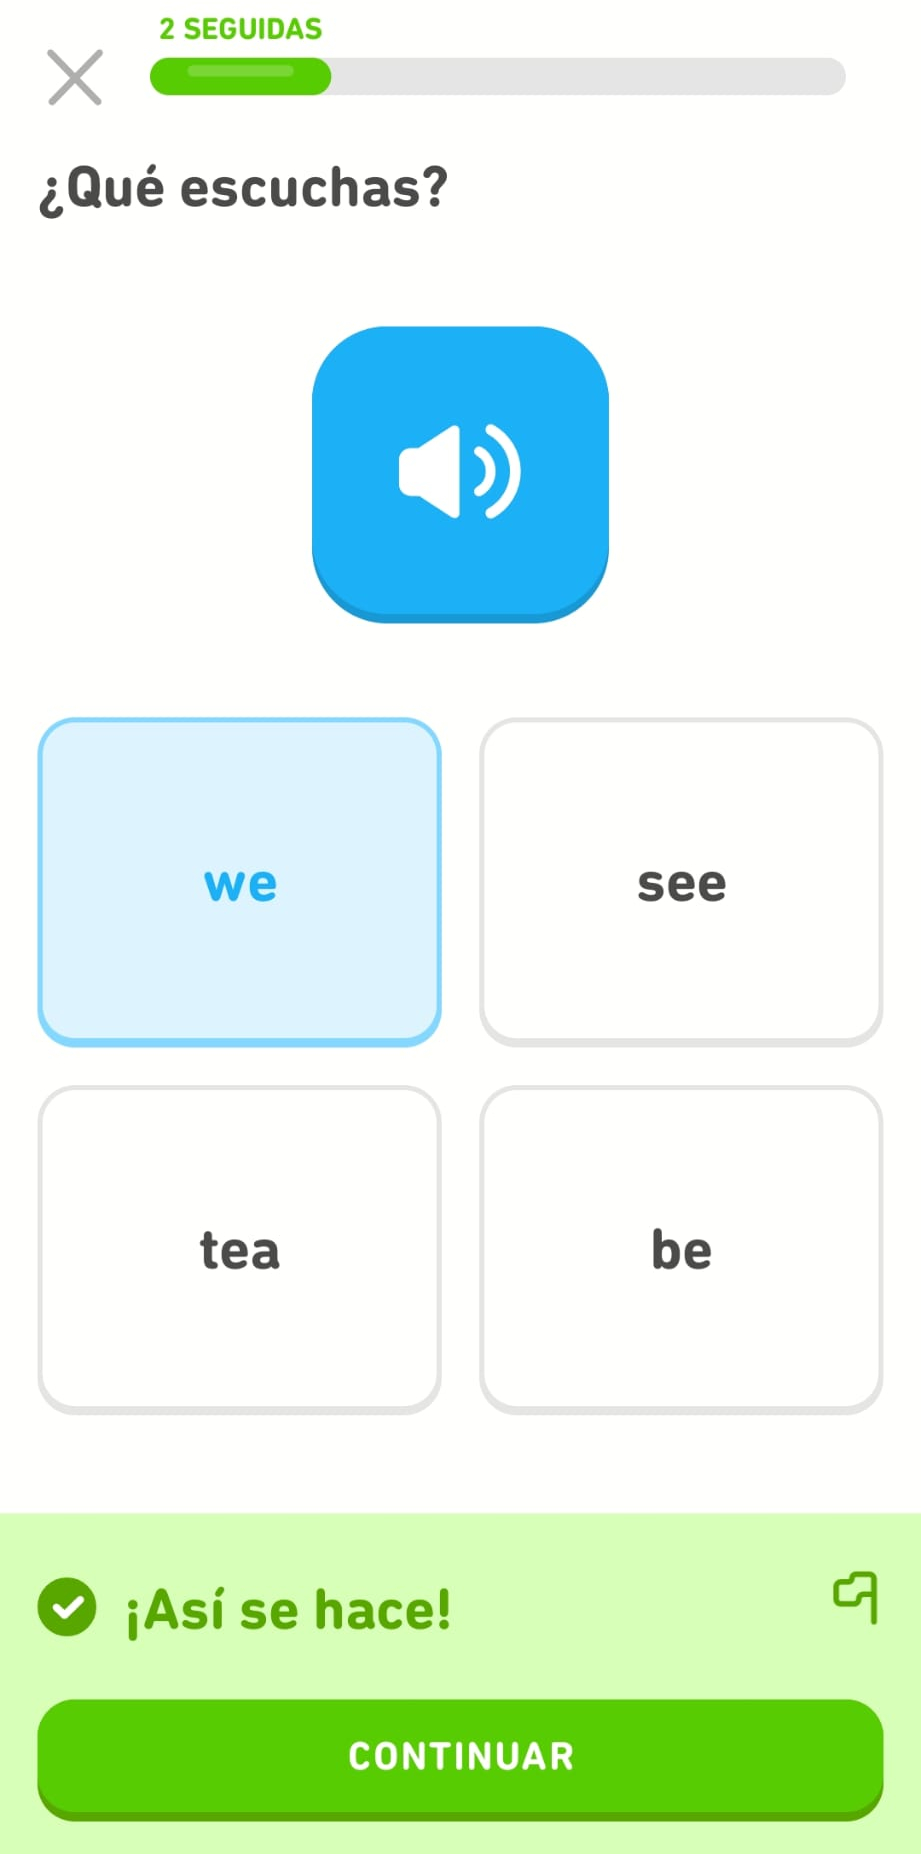
\includegraphics[width=0.33\textwidth]{imagenes/c2/duolingo.jpeg}
    \caption{Ejercicio de Duolingo donde el usuario debe adivinar qué palabra corresponde al audio}
    \label{fig:duolingo}
\end{figure} 


\subsubsection{Artly}
Artly es una aplicación móvil que permite aprender cientos de obras de arte de forma interactiva. De forma parecida a Duolingo, 
cuando el usuario abre la aplicación, se encuentra una lista de secciones (Figura \ref{fig:artly}) correspondientes a los distintos movimientos 
artísticos. Estos apartados se irán desbloqueando uno a uno a medida que el usuario vaya completando las lecciones y ejercicios.
 
En cada uno de los apartados el usuario podrá ver una lista de cuadros y esculturas de los distintos artistas que pertenecen a ese movimiento.
Al seleccionar uno de ellos, se abrirá una pantalla con la imagen del cuadro o escultura, en la que el usuario podrá ver la obra más de cerca, junto
con el título, el autor y una descripción. 
Artly incorpora además una serie de preguntas sobre las obras vistas en dicho apartado (seleccionar el autor, seleccionar el título de la obra...). 
Al finalizar las preguntas, el usuario sumará un progreso en el tema que permitirá desbloquear otros apartados y conseguir ciertos logros en su perfil.
La aplicación es gratuita pero tiene mejoras de pago que te permitirán avanzar con más facilidad y sin anuncios.

\begin{figure}[H]

    \centering
    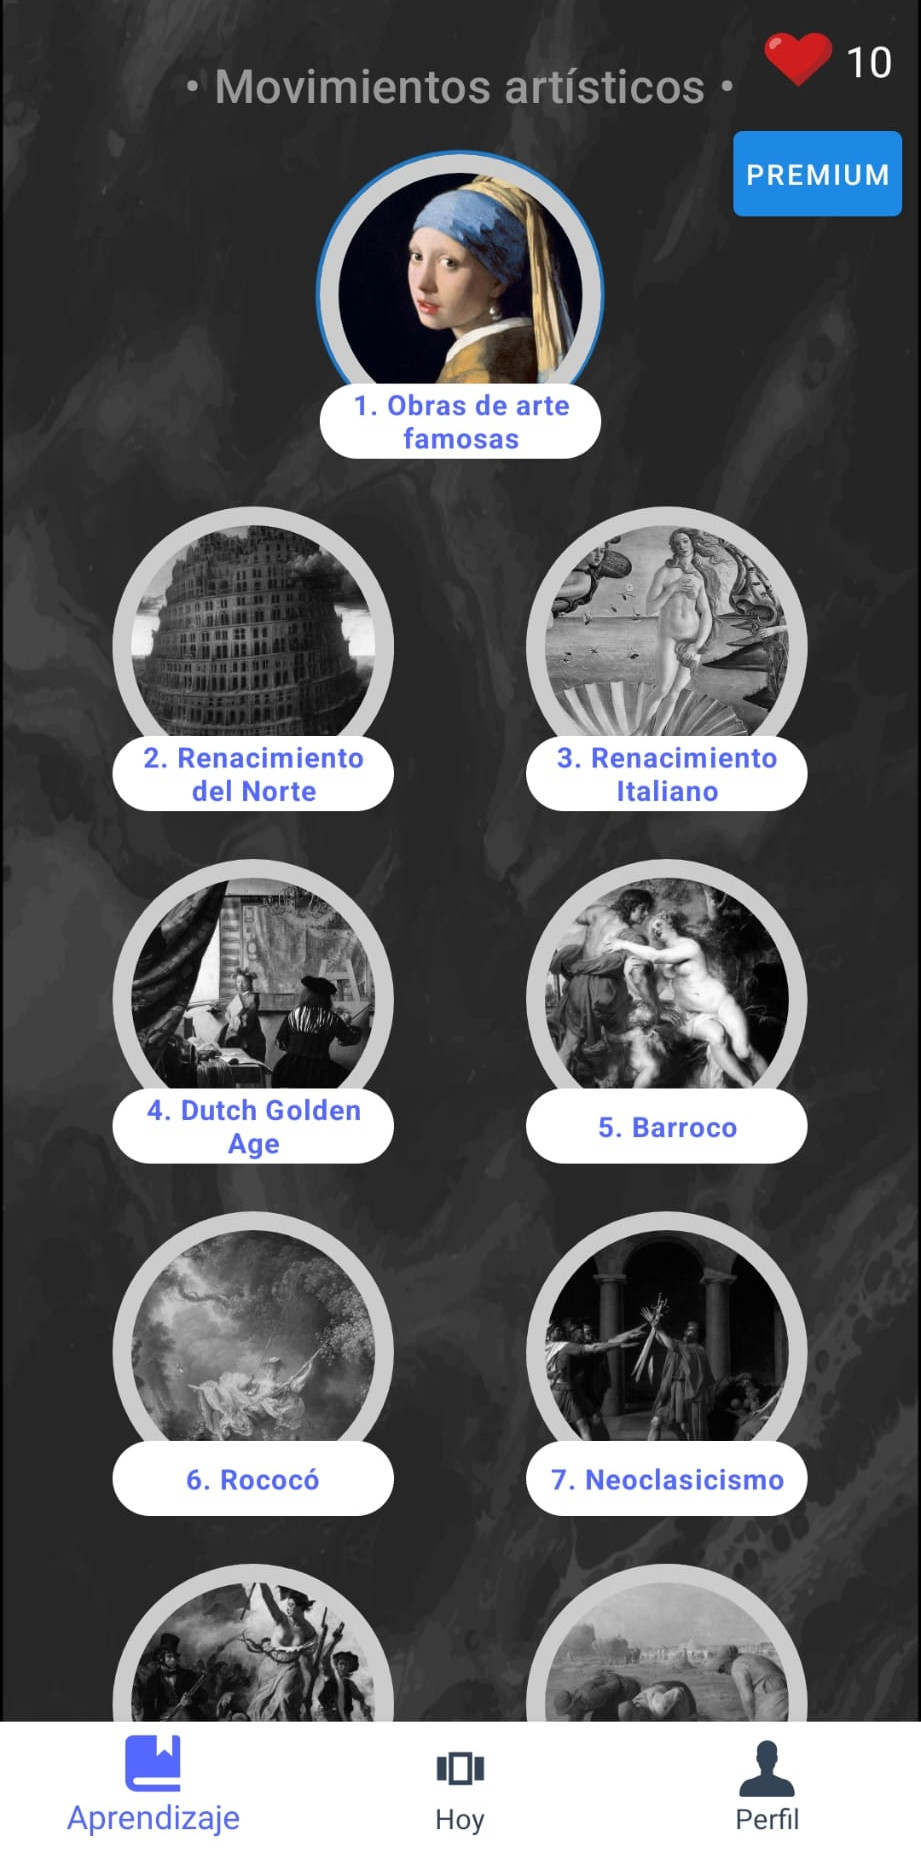
\includegraphics[width=0.4\textwidth]{imagenes/c2/artly.jpeg}
    \caption{Menú de selección de las lecciones de Artly clasificadas en movimientos artísticos}
    \label{fig:artly}

\end{figure}



\subsubsection{BMath}
BMath es un software para móviles para el aprendizaje de conceptos matemáticos mediante gamificación. Esta aplicación crea un programa personalizado para el
usuario en función del curso académico en el que esté, adaptándose a su conocimiento y a su nivel. Pese a ser gratuita, el tiempo diario que te permite el
modo básico es de 5 mintuos, mientras que si pagas te permitirá ampliarlo en 10 minutos cada día. 

Es un ejemplo de aprendizaje por gamificación ya que la aplicación es prácticamente un videojuego (de hecho, se consideran así), pues muestra una ciudad
(Figura \ref{fig:bmath}) por la que puedes mover la cámara y donde construyes distintos edificios. Para construirlos, deberás superar
una serie de pruebas sobre álgebra, geometría, etc. También obtendrás puntos de experiencia al superar los ejercicios(Figura \ref{fig:bmath2}) y, al subir de nivel, recibirás nuevos edificios y decoraciones para tu ciudad.
Con esto, se pretende que el usuario tenga la motivación de realizar ejercicios y superarlos correctamente para lograr que su ciudad.
prospere. Como alumno también puedes elegir tu propio personaje animado que te identificará en el juego.

Los diseños del software están muy cuidados y posee colores muy llamativos para que el usuario se sienta motivado y atraido. Además, la aplicación proporciona una experiencia 
de usuario agradable y motivadora, ayudando al alumno en todo momento 
a solucionar los ejercicios y enseñándole técnicas para resolverlos.

La aplicación también posee otras funciones como un apartado donde añadir recordatorios para acceder a la aplicación, preguntas para conocer cómo se siente el usuario tras cada sesión de estudio, sección parental, etc.

\begin{figure}[H]
    \centering
    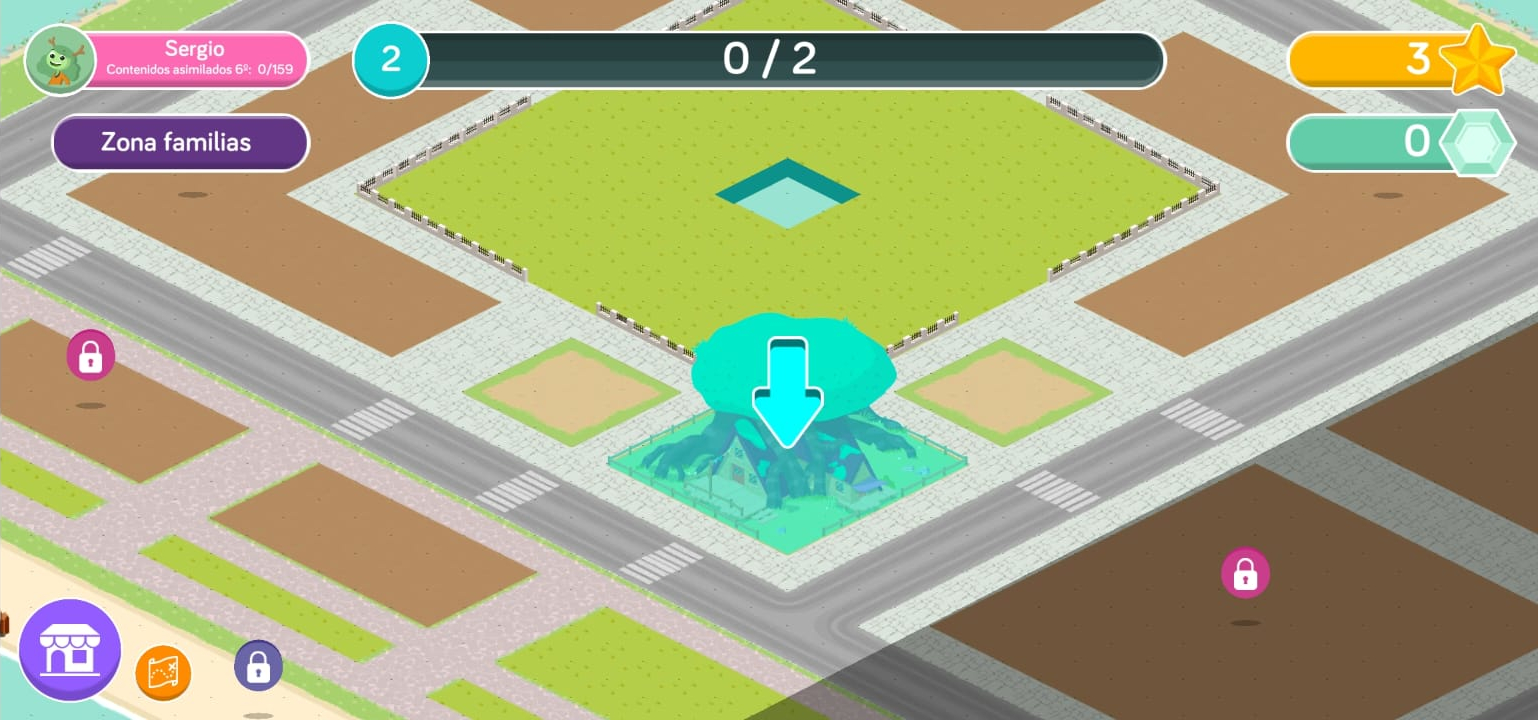
\includegraphics[width=\textwidth]{imagenes/c2/bmath.jpeg}
    \caption{Ciudad de BMath donde se seleccionan los niveles y se construyen los edificios para mostrar el progreso del usuario}
    \label{fig:bmath}

\end{figure}

\begin{figure}[H]
    \centering
    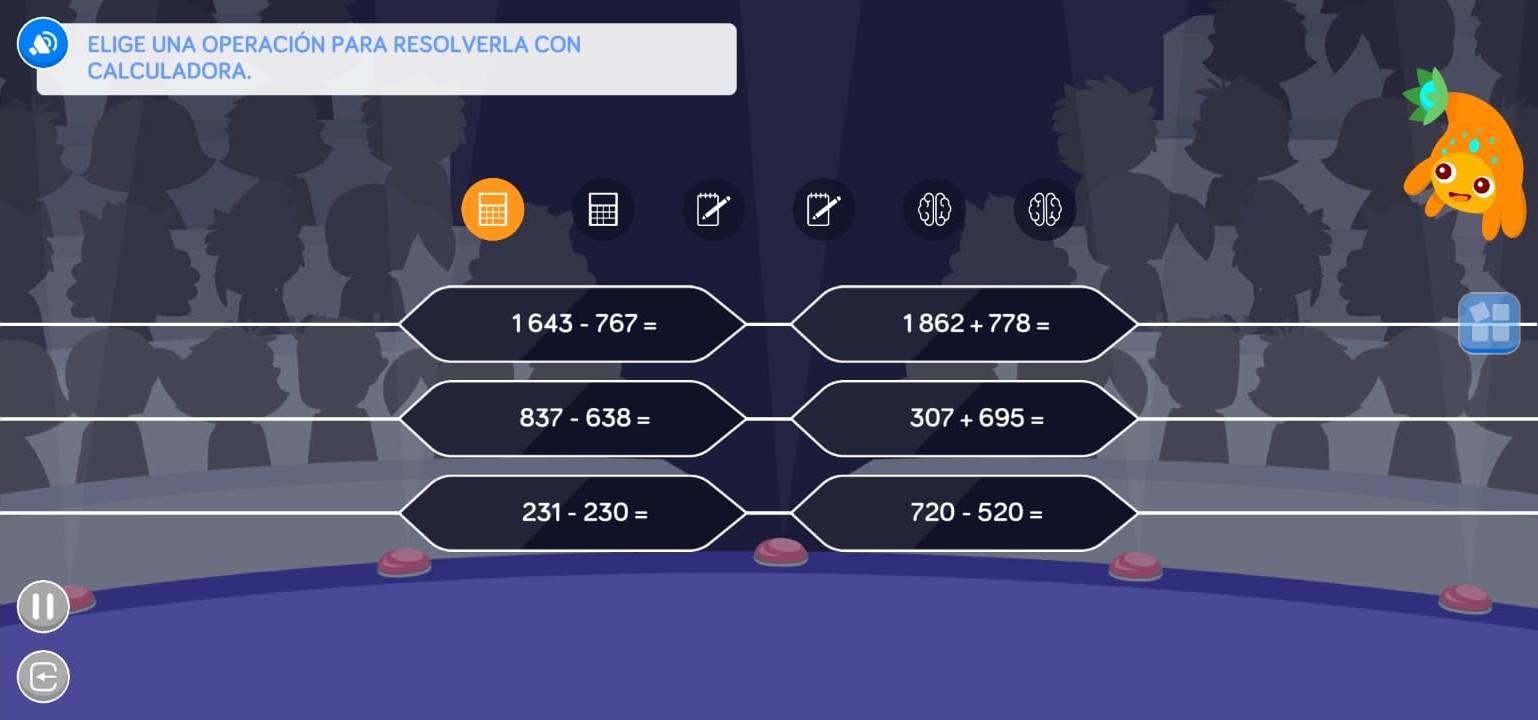
\includegraphics[width=\textwidth]{imagenes/c2/bmath2.jpeg}
    \caption{Ejercicio de BMath sobre cálculo matemático (sumas y restas) con calculadora, con papel y mentalmente}
    \label{fig:bmath2}

\end{figure}


\newpage

\subsection{Aplicaciones de aprendizaje musical}
Centrándonos ya en el tema que nos ocupa (el aprendizaje musical) existen numerosas aplicaciones que ayudan a la adquisición
de conocimientos musicales o a la ayuda a aprender a tocar un instrumento musical. A continuación se muestran algunas de ellas.


\subsubsection{Curso de Lenguaje Musical}
Esta herramienta para móvil tiene el objetivo de enseñar los conceptos básicos de lenguaje musical. La aplicación proporciona una forma de aprendizaje muy 
tradicional y que no está basada en la gamificación, ya que no dispone de ningún tipo de seguimiento del progreso ni de ejercicios para realizar sobre las lecciones aprendidas.
La app contiene una lista de lecciones (Figura \ref{fig:clm}) y cada una de ellas muestra un vídeo de un docente explicando el contenido del temario. 

Por último, en cuanto a la interfaz, la aplicación es muy sencilla y tiene un diseño poco atractivo, dando una simple lista con enlaces
a los vídeos de las lecciones sin ningún tipo de decoración o imagen.

\begin{figure}[H]
    \centering
    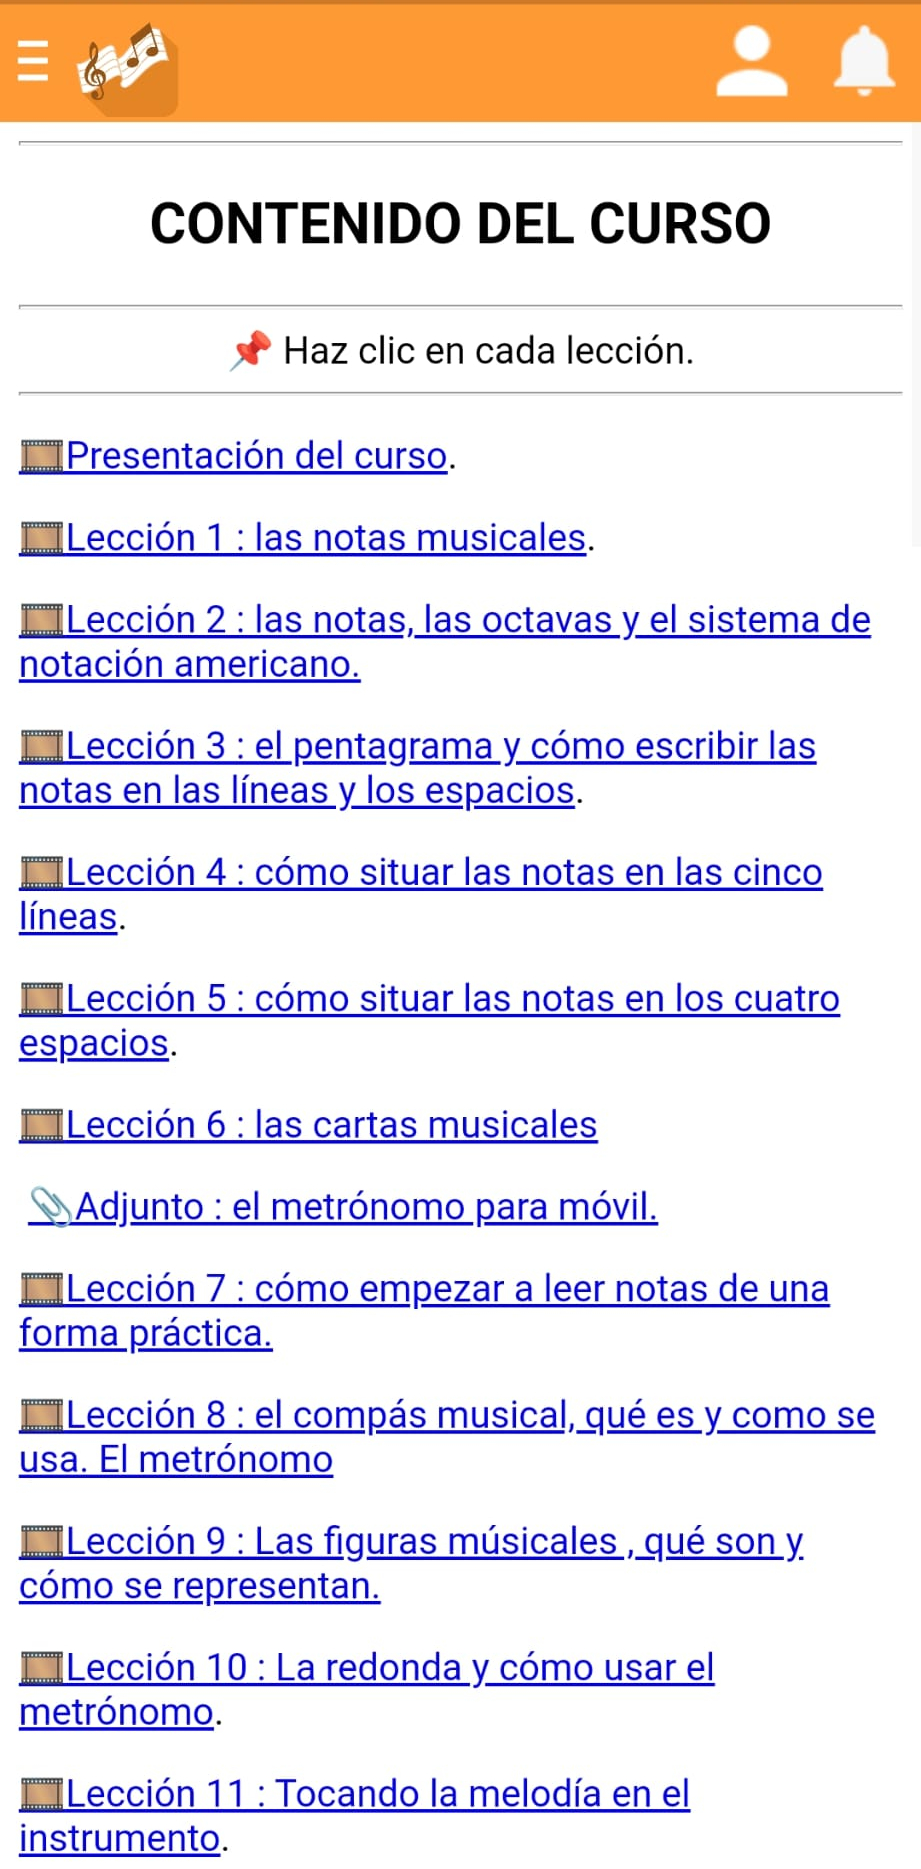
\includegraphics[width=0.4\textwidth]{imagenes/c2/cursomusica.jpeg}
    \caption{Lista de lecciones que ofrece la aplicación Curso de Lenguaje Musical}
    \label{fig:clm}
\end{figure}


\subsubsection{Sonid}
Sonid consiste en una aplicación para el aprendizaje de piano a través de la gamificación.
La aplicación se divide en distintas lecciones (Figura \ref{fig:sonid2}) que el usuario irá desbloqueando al pasarlas correctamente.
Cada lección explica unos conceptos básicos de música y piano y, al finalizar, el usuario deberá realizar una serie
de ejercicios para comprobar que ha entendido y aprendido el contenido del temario.

Algunos de los ejercicios que posee esta aplicación son:
\begin{itemize}
    \item Seleccionar la tecla en el piano que corresponde a una nota musical. (Figura \ref{fig:sonid})
    \item Responder si la tecla que se ha pulsado es una nota musical o no.
    \item Decidir qué nota musical corresponde a una tecla del piano que se ha pulsado.
\end{itemize}

Además de las lecciones, el usuario también puede practicar con escalas y acordes del piano, asi como aprenderlas en la wiki y en el diccionario que 
posee la aplicación. También dispone de un foro para que toda la gente pueda compartir sus dudas.

Por último, en cuanto al seguimiento, el usuario puede ver su progreso y sus estadísticas en su perfil, donde aparece el número de lecciones
completadas, el número de errores que ha tenido, la experiencia que tiene. Además, el usuario consigue logros al completar las lecciones y 
comparte una clasificación global con otros usuarios que también usan la aplicación.

% \subsubsection{--}

\begin{figure}[H]
    \centering
    \subfloat[\centering Ejercicio de Sonid para conocer las notas de un piano]{\label{fig:sonid}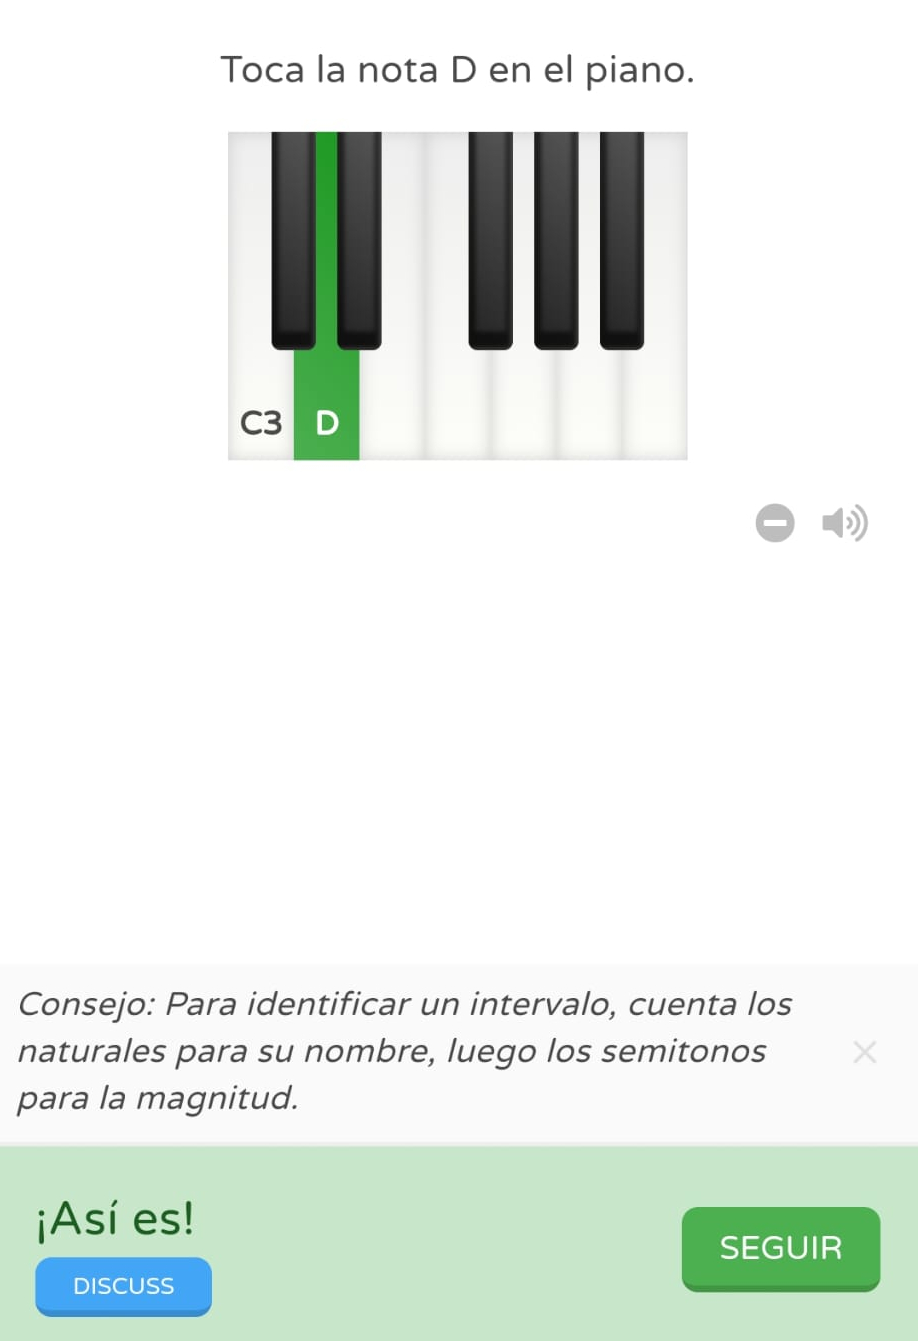
\includegraphics[width=0.35\textwidth]{imagenes/c2/sonid.jpeg}}
    \hspace{3em}
    \subfloat[\centering Menú de selección de lecciones de Sonid dividido por escalas]{\label{fig:sonid2}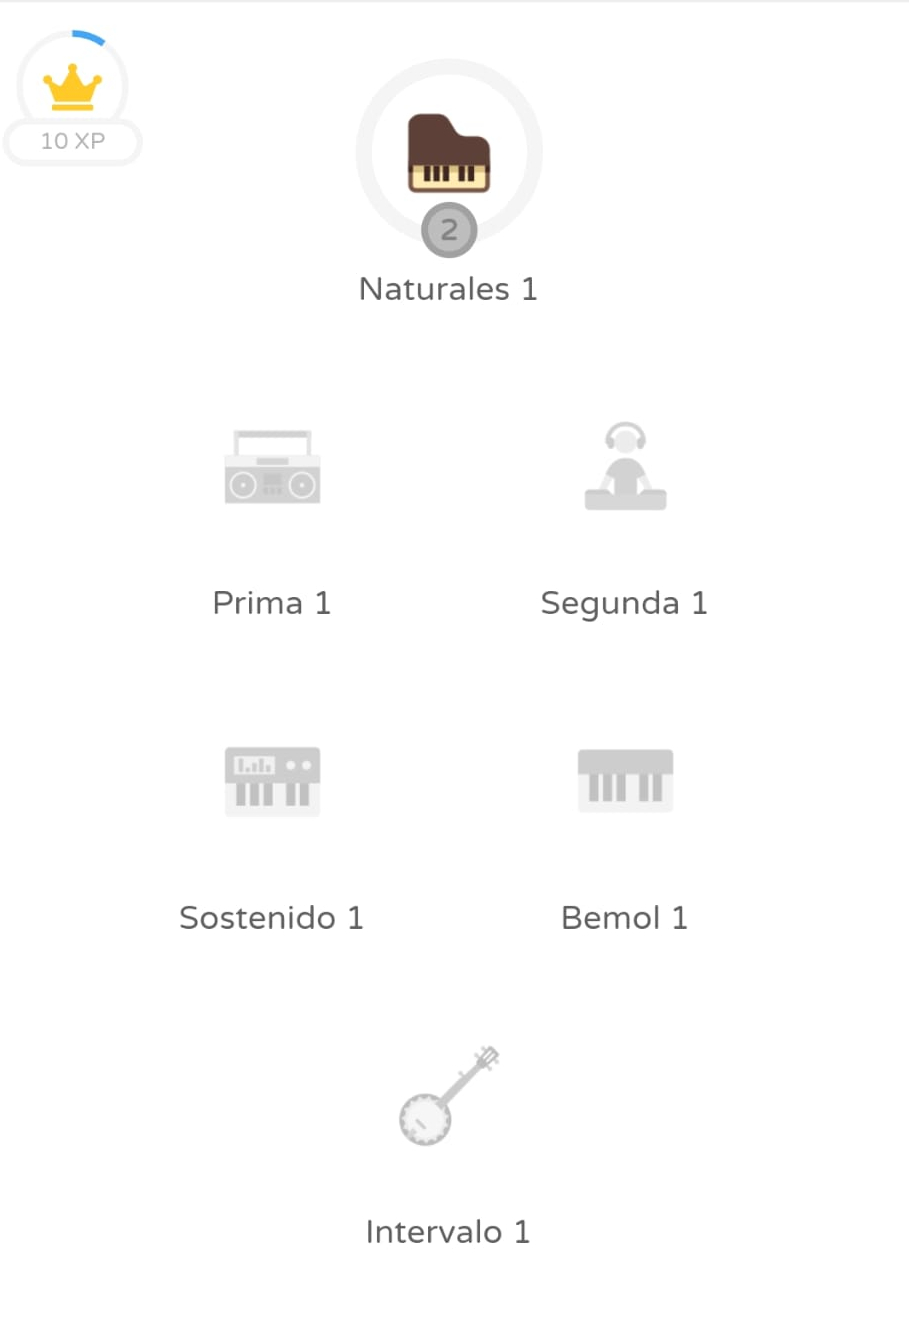
\includegraphics[width=0.35\textwidth]{imagenes/c2/sonid1.jpeg}}
\end{figure}

\newpage



\section{Desarrollo de Software}

\subsection{Flutter}
\begin{wrapfigure}{r}{0.27\textwidth}
\vspace*{-0.4cm}
\centering

\includegraphics[width=0.27\textwidth]{imagenes/c2/flutter.png}

\caption{Logo de Flutter}
\end{wrapfigure}Flutter es un kit de desarrollo software (framework) de código abierto destinado al desarrollo de aplicaciones móviles multiplataforma. Está programado en Dart, fue creado por Google y su primera versión estable se lanzó en 2018.
Se emplea para desarrollar aplicaciones para móvil, web y escritorio desde una sola base de código, lo cual permite mucha más agilidad y consistencia.

Flutter ofrece tres ventajas respecto a otros frameworks utilizados para el desarrollo de aplicaciones multiplataformas:

\begin{itemize}
\item \textbf{Compilación en nativo}
\item \textbf{Flexibilidad} para crear interfaces gráficas
\item \textbf{Desarrollo veloz}, permitiendo ver el resultado del código al instante.

\end{itemize}
Flutter está basado en el concepto de widgets, que son los elementos que componen la interfaz y la interacción del usuario. Estos widgets pueden ser modificados, añadidos o eliminados
dinámicamente, permitiendo una gran flexibilidad a la hora de crear interfaces gráficas. 

\subsection{React Native}
Framework de código abierto creado por Meta Platforms (Facebook) y destinado al desarrollo de aplicaciones muliplataforma para Android, iOS, Web, Windows, etc.
Está basado en Javascript como lenguaje de programación y en React como herramienta para la interfaz de usuario. La diferencia con React es que, en lugar de 
trabajar con el navegador, trabaja con las plataformas móviles al transformar los componentes en nativos en función de la plataforma en la que se esté
ejecutando la aplicación. 

Esta tecnología permite construir aplicaciones móviles usando solamente Javascript, con el mismo diseño que utiliza
React permitiendote realizar una interfaz de usuario completa mediante componentes. 


\begin{figure}[H]
\centering

\includegraphics[width=0.3\textwidth]{imagenes/c2/reactnative.png}
\caption{Logo de React Native}
\end{figure}


Podemos encontrar dos ventajas en este framework:

\begin{itemize}
\item \textbf{Código compartido:} tu código puede ser compartido para diferentes plataformas.
\item \textbf{Comunidad:} Existe una amplia comunidad sobre React y React Native, lo cual permite encontrar soluciones a los problemas que se puedan presentar en el desarrollo.
\end {itemize}

Como desventaja, encontramos una limitación en los componentes nativos, pues seguramente se necesite escribir algo de código
específico para un plataforma en concreto


\begin{wrapfigure}{r}{0.27\textwidth}
    \vspace*{-0.4cm}

    \centering
    
\includegraphics[width=0.27\textwidth]{imagenes/c2/dart.png}
    \caption{Logo de Dart}
\end{wrapfigure}\subsection{Dart}
Dart es un lenguaje de programación de código abierto desarrollado por Google y utilizado por Flutter.
Es orientado a objetos y de tipado estático. Surgió en 2011 como alternativa a Javascript.

Dart posee las siguientes ventajas:

\begin{itemize}
\item \textbf{Lenguaje fácil y sencillo} de aprender
\item \textbf{Acceso gratuito}
\item \textbf{Funciona en todas las plataformas}
\item \textbf{Programación estructurada y flexible}
\item Al ser \textbf{orientado a objetos}, facilita la encapsulación y reutilización de código gracias al uso de clases.
 
\end{itemize}

\subsection{Kotlin}
Kotlin es un lenguaje de programación construido sobre Java, desarrollado por JetBrains y lanzado en 2016.
Es orientado a objetos y tiene tipado estático, pero también soporta la programación por procedimientos y funciones. 

Algunas de sus ventajas son:
\begin{itemize}
\item \textbf{Compatibilidad con Java:} permite utilizar código Java en Kotlin y viceversa
\item \textbf{Lenguaje fácil y sencillo} de aprender y usar por su sintáxis similar a Java
\item \textbf{Robusto:} Es un lenguaje seguro con los valores nulos 
\item \textbf{Exactitud y claridad}: reduce el código repetido de forma sustancial y disminuye la probabilidad de error.

\end{itemize}


\subsection{NodeJS}
NodeJS es un entorno en tiempo de ejecución de código abierto, del lado del servidor y programado en Javascript. 
Es asíncrono y dirigido por eventos. Node es utilizado para el desarrollo de aplicaciones de red escalables y rápidas, ofreciendo beneficios
en rendimiento, velocidad de desarrollo, etc. 

Se utiliza en el desarrollo de aplicaciones web porque permite ejecutar Javascript del lado del servidor en lugar de en el navegador. 

Los principales motivos para utilizar NodeJS son:
\begin{itemize}
    \item \textbf{Simultaneidad de peticiones}: NodeJS es capaz de manejar múltiples peticiones al mismo tiempo gracias al modelo dirigido por eventos, 
    lo que permite una mayor escalabilidad.
    \item \textbf{Lenguaje sencillo} basado en Javascript.
    \item \textbf{Gestión de paquetes de calidad} gracias a NPM.
\end{itemize}


\subsection{React}
React es una biblioteca Javascript de código abierto que se utiliza para la creación de interfaces de usuario de forma fácil y sencilla.
Es mantenida por una gran comunidad de desarrolladores de software libre y fue lanzada en 2013. 

En React se trabaja con componentes, los cuales son elementos o partes de la interfaz de usuario que facilitarán la reutilización de código y la modularidad.

Entre las ventajas de React encontramos:
\begin{itemize}
\item \textbf{Componentes reutilizables:} React permite crear componentes que pueden ser reutilizados en otras partes de la aplicación.
\item \textbf{Fácil de aprender:} React es fácil de aprender y de utilizar, además de tener una documentación sólida y una gran cantidad de recursos online gratuitos.
\item \textbf{Rendimiento:} React es rápido y eficiente gracias al DOM virtual.
\end{itemize}

\subsection{Angular}
Angular es un framework de código abierto para el desarrollo de aplicaciones web y móviles. Está basado en TypeScript y está desarrollado por Google.
Esta tecnología también está basada en componentes, lo cual permite la creación de aplicaciones web escalables

\subsection{MongoDB}
MongoDB es una base de datos no relacional de código abierto y orientada a documentos. 
Es de tipo NoSQL, es decir, que no utiliza el modelo relacional de bases de datos tradicionales.
Cada registro de la base de datos es un documento que consta de pares clave - valor (muy similar a los objetos JSON).
Está escrito en C++ y las consultas se hacen pasando objetos JSON como parámetros.

MongoDB proporciona las siguientes ventajas:
\begin{itemize}
\item \textbf{Rendimiento:} MongoDB es más rápido porque almacena los datos directamente en un mismo sitio (colección).
\item \textbf{Simplicidad:} No hay que seguir un esquema ni unir tablas como en SQL.
\item  \textbf{Flexibilidad} para diseñar el esquema y crear las relaciones.
\end{itemize}
\begin{figure}[H]
    \centering
    
\includegraphics[width=0.4\textwidth]{imagenes/c2/mongodb.png}
    \caption{Logo de MongoDB}
\end{figure}

\subsection{Pilas MERN \& MEAN}
MERN es un conjunto de tecnologías que se utilizan para el desarrollo de aplicaciones web. Está compuesto por las siglas de MongoDB, Express (ayuda para crear y gestionar el backend en Node), React y NodeJS. MEAN es igual, pero sustituye React por
Angular. 

Hay una gran cantidad de beneficios al utilizar una de estas pilas para desarrollar una aplicación web como por ejemplo:
\begin{itemize}
\item \textbf{Cubre todo el ciclo de desarrollo}: Desde el backend hasta el frontend.
\item \textbf{Facilita el trabajo} con la arquitectura modelo-vista-controlador.
\item \textbf{Rápido desarrollo:} El desarrollo de una aplicación web con estas tecnologías es rápido y eficiente.
\item \textbf{Código abierto}: Todas las tecnologías que componen estas pilas son de código abierto y gratuitas y están respaldadas por la comunidad.
\item \textbf{Fácil mantenimiento:} El mantenimiento de una aplicación web con estas tecnologías es fácil y sencillo.
\end{itemize}

\begin{figure}[H]
    \centering
    
\includegraphics[width=0.8\textwidth]{imagenes/c2/MERN.png}
    \caption{Pilas MEAN y MERN}
\end{figure}

\subsection{MariaDB}
MariaDB es un sistema de gestión de bases de datos relacional de código abierto. Es un fork de MySQL y está desarrollado por su comunidad de usuarios. Surgió en 2009 como
consecuencia de la compra de MySQL por parte de Sun Microsystems.
Sigue un modelo relacional, lo cual significa que el contenido de los datos se almacena en tablas con un esquema más rígido que en MongoDB u otra base de datos noSQL.

Pese a haber mencionado solamente MariaDB como ejemplo de sistema de gestión de bases de datos relacional, existen muchos otros como por ejemplo PostgreSQL, MySQL, etc.


\begin{figure}[H]
    \centering
    
\includegraphics[width=0.4\textwidth]{imagenes/c2/mariadb.png}
    \caption{Logo de MariaDB}
\end{figure}

   \chapter{Especificación de requisitos}


\section{Introducción}
A continuación, vamos a describir y detallar los requisitos del sistema 
que vamos a desarrollar. En esta sección se describirá qué vamos a construir y cómo lo vamos
a hacer, con sus restricciones específicas.

\subsection{Propósito}
En este capítulo se pretende describir de forma clara y precisa las funciones, carasterísticas y restricciones 
del sistema que se va a desarrollar. Estas definiciones servirán al equipo de desarrolo para 
conocer las necesidades del sistema y a los usuarios finales. 

Además, este documento servirá como base para el desarrollo de las funcionalidades descritas y como medio de comunicación 
entre las partes involucradas en el proyecto.
\subsection{Ámbito del Sistema}
El sistema que vamos a desarrollar es una aplicación multiplataforma llamada "Meloudy" que permitirá a los usuarios
aprender conceptos musicales de una forma amena y divertida. La aplicación llevará el progreso de los usuarios que les permitirá saber cómo van en su aprendizaje.

Las gestiones que se realizarán en el sistema son:
\begin{itemize}
    \item \textbf{Gestión de usuarios: } El sistema permitirá a los administradores crear y eliminar usuarios, además de modificar sus datos. Los usuarios también podrán
    modificar sus datos.
    \item \textbf{Gestión de lecciones: } El sistema facilitará la modificación de los textos de las lecciones y de las preguntas asociadas a estas.
\end{itemize}


\subsection{Definiciones, Acrónimos y Abreviaturas}
A continuación se detallará el significado de algunos conceptos importantes para la comprensión del documento y de nuestro sistema.
\begin{itemize}
    \item \textbf{Requisito:} Es una condición o característica que debe cumplir el sistema para satisfacer una necesidad o cumplir una función.
    \item \textbf{Funcionalidad:} Descripción de lo que debe hacer el producto software.
    \item \textbf{Restricción:} Condición que limita la funcionalidad del sistema.
    \item \textbf{Interfaces externas:} Tipo de requisito que incluye la interfaz de usuario (interacción entre el software y el usuario), los diseños de pantallas, las interfaces hardware y software, etc.
    \item \textbf{Usuario: }Persona que utilizará la aplicación para la intención final de esta.
    \item \textbf{Administrador: } Persona encargada del sistema software y del mantenimiento de este para su buen funcionamiento.
    \item \textbf{RF / RNF:} Requisito funcional / Requisito No Funcional.
\end{itemize}

\subsection{Referencias}
Esta sección de Especificación de requisitos ha sido redactada consultando los documentos del estándar IEEE Recommended Practice for Software Requirements Specification ANSI/IEEE 830, 1998.

\subsection{Visión General del Documento}
El documento consta de tres partes bien diferenciadas:
\begin{itemize}
    \item \textbf{Introducción:} Proporciona una visión general sobre el apartado de Especificación de Requisitos sin profundizar en los requisitos como tal.
    \item \textbf{Descripción General:} Se describirá el sistema a construir para saber las funciones principales, los datos necesarios, las restricciones y otros aspectos que puedan afectar al desarrollo de la aplicación.
    \item \textbf{Requisitos Específicos:} Se profundiza en las necesidades del usuario definiendo los requisitos que debe tener nuestro sistema tras el desarrollo y la implementación de este.
\end{itemize}

\section{Descripción General}
A continuación, se procederá a describir con poco detalle los requisitos del sistema de una forma general para saber las funciones principales a desarrollar, las características de los usuarios, las dependencias, etc.
\subsection{Perspectiva del producto}
Se pretende implementar un sistema que permita el aprendizaje del usuario mediante técnicas de gamificación y ejercicios a resolver. Algunas de estas actividades utilizarán librerías para la detección de notas musicales
a partir de la frecuencia captada por el micrófono del usuario y, por tanto, la aplicación dependerá de dichas librerías que se incluyan.
Por otro lado, el sistema de administración y el progreso de los usuarios se llevará a cabo utilizando una base de datos en la que se almacenará la información necesaria de los usuarios y su progreso.

La interacción de los usuarios con la aplicación será mediante una interfaz gráfica que podrá ser utilizada con la pantalla táctil o el ratón del dispositivo usado.

\subsection{Funciones del producto}
Las principales funciones que el usuario podrá realizar dentro de la aplicación son:
\begin{itemize}
    \item Selección de lecciones a aprender.
    \item Respuesta (mediante selección o escritura) de las preguntas y actividades que ofrezca la aplicación.
    \item Consulta del progreso individual, de los logros obtenidos y de la clasifiación global.
    \item Modificación de los datos del perfil.
\end {itemize}

Además, el encargado/profesor se encargará de parte de la administración de las lecciones mediante:
\begin{itemize}
    \item Modificación y creación del texto de la lección
    \item Modificación de las preguntas y actividades
    \item Creación de preguntas para una lección
\end{itemize}

\subsection{Características de los usuarios}
Los usuarios que usarán la aplicación tendrán distintos perfiles y abarcarán edades muy distintas. Aún así,
el perfil objetivo para el uso del sistema será las personas jóvenes, pues suelen utilizar mucho más las nuevas tecnologías
y estarán más familiarizados con este tipo de aplicaciones. No se necesita conocimiento musical previo para utilizar el software y, 
de hecho, las lecciones pueden ser bastante básicas y sencillas para las personas que ya conozcan conceptos y aspectos avanzados del lenguaje musical.


\subsection{Restricciones}
\subsection{Suposiciones y dependencias}


\section{Requisitos Específicos}
\subsection{Requisitos funcionales}
\subsection{Requisitos no funcionales}
\subsection{Requisitos de información}
\subsection{Bocetos de interfaz de usuario}

   \chapter{Planificación}

\section{Introducción}
En este capítulo se describirá la planificación para el desarrollo del proyecto, la cual va a servir para poder
realizar un control de los avances del producto y asegurar que se cumplan los objetivos marcados en cada sprint/iteración.
Para ello, se utilizarán ciertos elementos de la metodología SCRUM, el cual definiremos brevemente a continuación:



\subsection*{SCRUM}
SCRUM es un marco de trabajo iterativo e incremental que se utiliza para desarrollar proyectos de software.
Este marco de trabajo se basa en la idea de que el desarrollo de software es un proceso complejo que se adapta continuamente
a las circunstancias. Por ello, se divide en pequeñas iteraciones que se van realizando de forma incremental y utiliza una serie de elementos
para poder controlar el desarrollo del proyecto:
\begin{itemize}
    \item \textbf{Artefactos:} Son documentos que se utilizan para controlar el desarrollo del proyecto.
    \item \textbf{Reuniones: } Se realizan cuatro tipos de reuniones de forma periódica para poder controlar y seguir el progreso del proyecto.
    \item \textbf{Roles:} Representan la responsabilidad de cada persona en el proceso.
\end{itemize}

\hfill

\begin{figure}[H]
    \centering
    \centerline{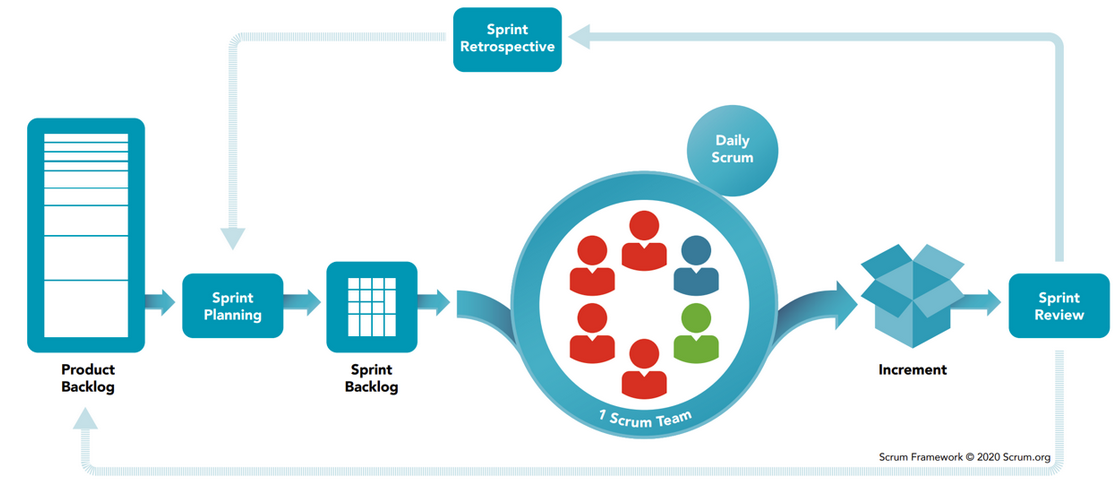
\includegraphics[width=\textwidth]{imagenes/c4/scrum.png}}
    \caption{Diagrama de la arquitectura del sistema, donde se muestra la comunicación entre el servidor y la aplicación móvil.}
    \label{fig:diagramadearquitectura}    
\end{figure}

Es importante recalcar que no voy a seguir la metodología SCRUM, sino que solo usaré algunos principios y
conceptos de metodologías ágiles debido a las condiciones en las que se va a desarrollar el proyecto
(no hay un cliente real, no hay un equipo de desarrollo real, etc.). Por tanto, se utilizarán los siguientes aspectos de SCRUM:
\begin{itemize}
    \item \textbf{Sprints:} Se definirán los Sprints (iteraciones) que se realizarán para el desarrollo del proyecto, explicando
          el objetivo de cada uno de ellos y detallando la duración y las fechas de inicio y de fin.
    \item \textbf{Historias de Usuario:} Se listarán y describirán las historias de usuario que se van a implementar en cada sprint a partir
          de los requisitos funcionales del proyecto especificados en el capítulo de Especificación de Requisitos.
    \item \textbf{Product Backlog: }Se definirá el product backlog, que es una lista de todas las funcionalidades (Historias de usuario) que se
          pretenden implementar en el proyecto. Esta lista se ordenará por prioridad de acuerdo a la importancia que tienen para el usuario final.
    \item \textbf{Velocidad:} Se calculará la velocidad de trabajo que se tendrá en el desarrollo del proyecto a partir de la cantidad de horas
          que se pretenden dedicar al proyecto cada día y la duración de los Sprints.
    \item \textbf{Puntos de historia: }Se asignarán los puntos de historia a cada historia de usuario para poder estimar la cantidad de trabajo
          que se debería realizar en cada sprint. Los valores de estos puntos de historia se calcularán a partir de la estimación de la complejidad de cada historia de usuario.
    \item \textbf{Reuniones: }Pese a no encajar exactamente en ninguna de las reuniones que hay en SCRUM, se realizarán reuniones cada dos semanas para
          poder controlar el progreso del proyecto y realizar un seguimiento de los avances. En estas reuniones se tratará:
            \begin{itemize}
                \item \textbf{Qué se ha hecho:} Se comentará el trabajo realizado desde la anterior reunión para comentar las posibles mejoras.
                \item \textbf{Qué falta por hacer: }Se comparará la planificación realizada para el Sprint con el trabajo realizado, comprobando qué cosas han podido faltar.
                \item \textbf{Qué se piensa hacer: }Se volverá a planificar si es necesario y se determinará qué trabajo se planea realizar durante el nuevo Sprint.
            \end{itemize}
\end{itemize}



\section{Velocidad}
A continuación vamos a estimar la velocidad inicial de trabajo que se tendrá en el desarrollo. Esta será una aproximación
que nos ayudará a estimar la cantidad de trabajo que se debería realizar en cada iteración. Sin embargo, esta podrá variar
y ajustarse a lo largo del proyecto en función de la cantidad de trabajo que se logre completar en cada sprint.

Para calcular la velocidad, vamos a considerar las horas de trabajo que se pretenden dedicar al proyecto cada día y tratar
de estimar cuanta cantidad de trabajo se podría realizar.

\begin{itemize}
    \item Partimos de un ``equipo de desarrollo'' de 1 miembro.
    \item Se pretende dedicar 5 horas al día de trabajo aproximadamente.
    \item Cada Sprint dura 2 semanas (14 días). Si cada día trabajamos 5 horas de forma aproximada, obtenemos un total de 70 horas
          en cada Sprint.
    \item En mi entorno, se estima que 1 PH son dos días de trabajo ideal (es decir, 10 horas).
          Esto significa que cada dos jornadas de trabajo real, se debería completar 1 PH. Sin embargo, en la realidad, esto no siempre
          es así ya que estamos realizando una aproximación.
    \item Si multiplicamos un programador por las 70 horas de trabajo y lo dividimos por el número de horas de trabajo por cada punto de historia
          (10 horas), obtenemos que deberíamos completar \textbf{7 PH} por sprint aproximadamente.
\end{itemize}

\textit{Nota: La duración de los Sprints puede variar en función de factores externos al proyecto. Pero se tratará de que duren
    2 semanas para seguir un ritmo de trabajo constante.}
    
\textit{Nota 2: Puesto que estamos realizando estimaciones y suposiciones para la planificación, esta está sujeta a cambios a
    lo largo del proyecto.}

\section{Product Backlog}
A continuación, se listarán todas las historias de usuario ordenadas por prioridad de acuerdo a la importancia que tienen para el usuario final del producto.
\begin{itemize}
    \item \textbf{HU1 - } Como usuario quiero registrarme en la aplicación para poder comenzar a utilizar sus funcionalidades. (Prioridad: Alta | Puntos de Historia: 2)
    \item \textbf{HU2 - } Como usuario quiero iniciar sesión en la aplicación para poder acceder a sus funcionalidades. (Prioridad: Alta | Puntos de Historia: 2)
    \item \textbf{HU6 - } Como usuario quiero seleccionar una lección para leer el temario. (Prioridad: Alta | Puntos de Historia: 1)
    \item \textbf{HU7 - } Como usuario quiero empezar un test de una lección. (Prioridad: Alta | Puntos de Historia: 1)
    \item \textbf{HU26 - } Como usuario quiero responder una pregunta de un test del tipo escritura de texto. (Prioridad: Alta | Puntos de Historia: 1)
    \item \textbf{HU31 - } Como usuario quiero ver todas las lecciones. (Prioridad: Alta | Puntos de Historia: 0.5)
    \item \textbf{HU8 - } Como usuario quiero responder una pregunta de un test del tipo selección múltiple. (Prioridad: Alta | Puntos de Historia: 1)
    \item \textbf{HU9 - } Como usuario quiero responder una pregunta de un test del tipo selección única. (Prioridad: Alta | Puntos de Historia: 1)
    \item \textbf{HU10 - } Como usuario quiero responder una pregunta de un test del tipo respuesta por micrófono. (Prioridad: Alta | Puntos de Historia: 8)
    \item \textbf{HU29 - } Como profesor y administrador quiero ver una lista de todas las preguntas. (Prioridad: Alta | Puntos de Historia: 0.5)
    \item \textbf{HU11 - } Como usuario quiero ver el resultado de un test. (Prioridad: Media | Puntos de Historia: 2)
    \item \textbf{HU13 - } Como usuario quiero ver mi progreso en las lecciones. (Prioridad: Media | Puntos de Historia: 2)
    \item \textbf{HU28 - } Como profesor y administrador quiero ver una lista de todas las lecciones. (Prioridad: Media | Puntos de Historia: 0.5)
    \item \textbf{HU14 - } Como profesor y administrador quiero crear una lección. (Prioridad: Media | Puntos de Historia: 1)
    \item \textbf{HU15 - } Como profesor y administrador quiero modificar el texto de una lección. (Prioridad: Media | Puntos de Historia: 2)
    \item \textbf{HU16 - } Como profesor y administrador quiero añadir contenido multimedia a una lección. (Prioridad: Media | Puntos de Historia: 2)
    \item \textbf{HU17 - } Como profesor y administrador quiero eliminar contenido multimedia de una lección. (Prioridad: Media | Puntos de Historia: 1)
    \item \textbf{HU27 - } Como profesor y administrador quiero añadir preguntas a un test del tipo entrada de texto. (Prioridad: Media | Puntos de Historia: 1)
    \item \textbf{HU18 - } Como profesor y administrador quiero añadir preguntas a un test del tipo selección múltiple. (Prioridad: Media | Puntos de Historia: 1)
    \item \textbf{HU19 - } Como profesor y administrador quiero añadir preguntas a un test del tipo selección única. (Prioridad: Media | Puntos de Historia: 1)
    \item \textbf{HU20 - } Como profesor y administrador quiero añadir preguntas a un test del tipo respuesta por micrófono. (Prioridad: Media | Puntos de Historia: 2)
    \item \textbf{HU21 - } Como profesor y administrador quiero eliminar preguntas de un test. (Prioridad: Media | Puntos de Historia: 0.5)
    \item \textbf{HU22 - } Como profesor y administrador quiero modificar preguntas de un test. (Prioridad: Media | Puntos de Historia: 1)
    \item \textbf{HU30 - } Como administrador quiero ver una lista de todos los usuarios. (Prioridad: Media | Puntos de Historia: 0.5)
    \item \textbf{HU24 - } Como administrador quiero modificar los datos de un usuario. (Prioridad: Media | Puntos de Historia: 2)
    \item \textbf{HU25 - } Como administrador quiero eliminar un usuario. (Prioridad: Media | Puntos de Historia: 0.5)
    \item \textbf{HU3 - } Como usuario quiero ver mis datos personales. (Prioridad: Media | Puntos de Historia: 1)
    \item \textbf{HU4 - } Como usuario quiero editar los datos de mi perfil. (Prioridad: Media | Puntos de Historia: 2)
    \item \textbf{HU23 - } Como administrador quiero crear un usuario. (Prioridad: Baja | Puntos de Historia: 1)
    \item \textbf{HU12 - } Como usuario quiero ver la lista de mis logros. (Prioridad: Baja | Puntos de Historia: 1)
    \item \textbf{HU5 - } Como usuario quiero ver con detalle uno de mis logros.  (Prioridad: Baja | Puntos de Historia: 1)
    \item \textbf{HU31 - } Como profesor y administrador quiero eliminar una lección. (Prioridad: Media | Puntos de Historia: 0.5)
    \item \textbf{HU32 - } Como administrador quiero ver una lista de todos los logros. (Prioridad: Media | Puntos de Historia: 0.5)
    \item \textbf{HU33 - } Como administrador quiero modificar un logro. (Prioridad: Media | Puntos de Historia: 0.5)
    \item \textbf{HU34 - } Como administrador quiero crear un logro. (Prioridad: Media | Puntos de Historia: 0.5)
    \item \textbf{HU35 - } Como administrador quiero eliminar un logro. (Prioridad: Media | Puntos de Historia: 0.5)
\end{itemize}

\section{Sprints}
Nuestro proyecto se pretende desarrollar en 14 Sprints. Cada Sprint tendrá una duración de 2 semanas, y se pretenden realizar una media
de 7 puntos de historia por Sprint. A continuación se especificará el contenido de cada Sprint con las fechas de inicio y fin de cada uno de ellos.

\subsection{Sprint \#1 - Documentación inicial}
\textit{24/11/2022   -   08/12/2022}\\

En este Sprint se realizará:
\begin{itemize}

    \item Definición del proyecto y del alcance.
    \item Redactar Capítulo 1 - Introducción.
    \item Redactar Capítulo 2 - Estado del Arte.
\end{itemize}
\subsection{Sprint \#2 - Documentación de requisitos}
\textit{08/12/2022   -   12/01/2023}\\

En este Sprint se planea realizar:
\begin{itemize}
    \item Revisión de la documentación inicial y corrección de errores.
    \item Redactar Capítulo 3 - Especificación de Requisitos.
\end{itemize}

\newpage

\subsection{Sprint \#3 - Documentación de HU}
\textit{12/01/2023   -   03/02/2023}\\

En este Sprint se realizará:
\begin{itemize}
    \item Revisión de la documentación de requisitos y corrección de errores.
    \item Redactar Capítulo 4 - Planificación.
    \item Redactar Capítulo 5 - Análisis del problema.
\end{itemize}
\subsection{Sprint \#4 - Diseño y comienzo del desarrollo}
\textit{03/02/2023   -   17/02/2023}\\

En este Sprint se terminará la documentación y comenzará el desarrollo con:
\begin{itemize}
    \item Revisión de la planificación y el análisis y corrección de errores.
    \item Redactar Capítulo 6 - Diseño.
    \item Preparación del backend para el desarrollo.
          \begin{itemize}
              \item Creación de la base de datos.
              \item Creación de los modelos, rutas y controladores del servidor con NodeJS.
          \end{itemize}
    \item Preparación del frontend para el desarrollo (creación de la aplicación de Flutter).
\end{itemize}

\subsection{Sprint \#5 - Registro y login de usuarios}
\textit{17/02/2023   -   03/03/2023}\\

En este Sprint se comenzará el desarrollo de la aplicación realizando las funcionalidades iniciales del usuario
que utilizará la aplicación, tales como el registro, el login, la selección de lección, etc.
\begin{itemize}
    \item HU1 - Como usuario quiero registrarme en la aplicación.
    \item HU2 - Como usuario quiero iniciar sesión en la aplicación.
    \item HU6 - Como usuario quiero seleccionar una lección para leer el temario.
    \item HU31 - Como usuario quiero ver todas las lecciones.
    \item HU28 - Como profesor quiero ver una lista de todas las lecciones.
\end{itemize}


\subsection{Sprint \#6 - Tests y progreso}
\textit{03/03/2023   -   17/03/2023}\\

Este Sprint tendrá como objetivo el desarrollo de los tests permitiendo al usuario responder a las preguntas y ver el resultado.
Además, podrá comprobar su progreso en cada lección y en la pantalla principal que muestra todas las lecciones (desbloqueando las correspondientes en su caso).
\begin{itemize}
    \item HU7 - Como usuario quiero empezar un test de una lección.
    \item HU26 - Como usuario quiero responder una pregunta de un test del tipo escritura de texto.
    \item HU8 - Como usuario quiero responder una pregunta de un test del tipo selección múltiple.
    \item HU9 - Como usuario quiero responder una pregunta de un test del tipo selección única.
    \item HU11 - Como usuario quiero ver el resultado de un test.
    \item HU13 - Como usuario quiero ver mi progreso en las lecciones.

\end{itemize}

\subsection{Sprint \#7 - Entrada de micrófono y detección de tono}
\textit{17/03/2023   -   31/03/2023}\\

En este Sprint se realizará la funcionalidad de la entrada de micrófono y la detección de tono. Puesto que la historia de usuario es muy grande y compleja, se reservará
un Sprint entero para su desarrollo. Para desarrollar esta funcionalidad, se utilizarán librerías de Flutter que permitan la entrada de audio y trabajar con el mismo.
\begin{itemize}
    \item HU10 - Como usuario quiero responder una pregunta de un test del tipo respuesta por micrófono.
\end{itemize}

\newpage
\subsection{Sprint \#8 - Funcionalidades del profesor con lecciones}
\textit{31/03/2023   -   14/04/2023}\\

En la octava iteración se comenzarán a realizar las funcionalidades relacionadas con el profesor y la gestión de las lecciones.
Además, puede que se necesite terminar la funcionalidad de la entrada de micrófono de la iteración anterior debido a que su estimación
supera los puntos de historia de un Sprint.


\begin{itemize}
    \item HU29 - Como profesor quiero ver una lista de todas las preguntas.
    \item HU14 - Como profesor quiero crear una lección.
    \item HU15 - Como profesor quiero modificar el texto de una lección.
    \item HU16 - Como profesor quiero añadir contenido multimedia a una lección.
    \item HU17 - Como profesor quiero eliminar contenido multimedia de una lección.
\end{itemize}

\subsection{Sprint \#9 - Funcionalidades del profesor con tests}
\textit{14/04/2023   -   28/04/2023}\\

En esta iteración se realizarán las funcionalidades relacionadas con el profesor y la gestión de los tests, tales como la creación, modificación y eliminación de las preguntas
de los distintos tipos. Además, se realizará la funcionalidad de ver todos los usuarios registrados en la aplicación.


\begin{itemize}
    \item HU27 - Como profesor quiero añadir preguntas a un test del tipo escritura de texto.
    \item HU18 - Como profesor quiero añadir preguntas a un test del tipo selección múltiple.
    \item HU19 - Como profesor quiero añadir preguntas a un test del tipo selección única.
    \item HU20 - Como profesor quiero añadir preguntas a un test del tipo respuesta por micrófono.
    \item HU21 - Como profesor quiero eliminar preguntas de un test.
    \item HU22 - Como profesor quiero modificar preguntas de un test.
    \item HU30 - Como administrador quiero ver una lista de todos los usuarios.
\end{itemize}


\subsection{Sprint \#10 - Funcionalidades del administrador}
\textit{28/04/2023   -   12/05/2023}\\

En la decima iteración se pretenden implementar todas las funcionalidades que tienen que ver con la administración de los usuarios, además de
dos historias relacionadas con el perfil propio del usuario.
\begin{itemize}
    \item HU24 - Como administrador quiero modificar los datos de un usuario.
    \item HU25 - Como administrador quiero eliminar un usuario.
    \item HU3 - Como usuario quiero ver los datos personales y los logros de mi perfil.
    \item HU4 - Como usuario quiero editar los datos de mi perfil.
    \item HU23 - Como administrador quiero crear un usuario.
    \item HU32 - Como administrador quiero ver una lista de todos los logros. 
    \item HU33 - Como administrador quiero modificar un logro.
    \item HU34 - Como administrador quiero crear un logro.
    \item HU35 - Como administrador quiero eliminar un logro.
\end{itemize}

\subsection{Sprint \#11 - Funcionalidades poco prioritarias y valor añadido}
\textit{12/05/2023   -   26/05/2023}\\

El objetivo de este Sprint es acabar todas las historias de usuario que quedan del product backlog y cuya prioridad es baja como lo es la interacción entre los distintos usuarios de la aplicación. Además, se añadirá una funcionalidad de valor añadido
en función del tiempo disponible y de las funcionalidades que se hayan podido implementar en los Sprints anteriores.
\begin{itemize}
    \item HU5 - Como usuario quiero ver la lista de mis logros.
    \item HU12 - Como usuario quiero ver con detalle uno de mis logros.
    \item Realizar mejoras de código y arreglar errores.
    \item Mejorar el diseño de la aplicación.
\end{itemize}

\subsection{Sprint \#12 - Mejoras de código}
\textit{26/05/2023   -   09/06/2023}\\

En este Sprint se pretende realizar mejoras de código en cuanto a estilo, formato y calidad del mismo. Además, se pretende dejar terminado la redacción
del séptimo capítulo del documento.
\begin{itemize}
    \item Revisar Capítulo 7 - Implementación
    \item Realizar mejoras de código y arreglar errores.
\end{itemize}

\subsection{Sprint \#13 - Pruebas }
\textit{09/06/2023   -   23/06/2023}\\

Este Sprint se dedicará a realizar todas las pruebas necesarias para comprobar que la aplicación funciona correctamente y que no hay errores en el código, tanto
en el frontend como en el backend. También se redactará el octavo capítulo del documento con las pruebas realizadas.

\begin{itemize}
    \item Realizar pruebas de integración.
    \item Realizar pruebas de unidad.
    \item Redactar Capítulo 8 - Pruebas.
\end{itemize}

\subsection{Sprint \#14 - Conclusión y finalización del proyecto}
\textit{23/06/2023   -   15/07/2023}\\

El último Sprint se dedicará por completo a la redacción del último capítulo del documento, en el que se recogerán las conclusiones del proyecto y se realizará una revisión
de todos los capítulos para corregir errores y mejorar la redacción. Se prepará también la presentación del proyecto para la defensa ante el tribunal.
\begin{itemize}
    \item Redactar Capítulo 9 - Conclusiones.
    \item Revisión de todo el documento y corrección de errores.
    \item Preparación de la presentación del proyecto.
\end{itemize}


\section{Diagrama de Gantt}
Por último, se muestran los diagramas de Gantt de la planificación del proyecto. 


El primero es más general y representa la división del desarrollo del producto en Sprints.
En él se puede ver la duración de cada Sprint y la proporción de estos en el tiempo total del proyecto. 

\begin{figure}[H]
    \centering
    \centerline{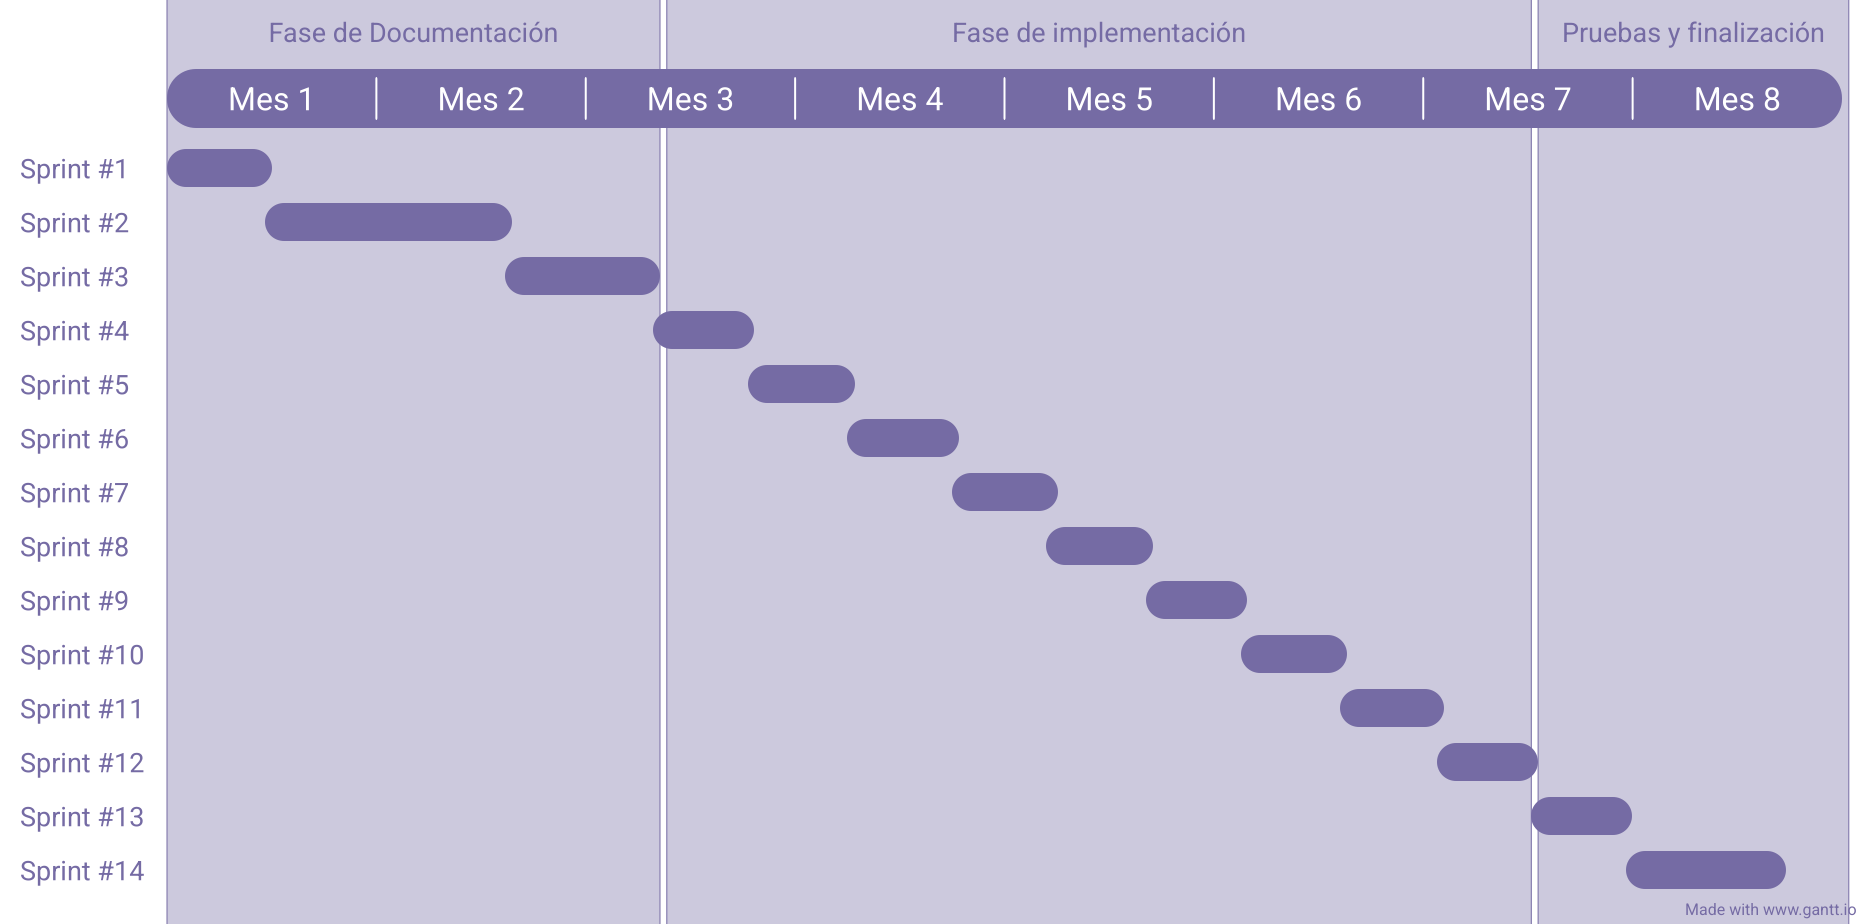
\includegraphics[width=1\textwidth]{imagenes/c4/gantt.png}}
    \caption{Diagrama de Gantt de la planificación del proyecto, divivido por Sprints.}
    \label{fig:diagrama_gantt}
\end{figure}

Como se puede ver, el proyecto se ha dividido en 14 Sprints, cada uno de ellos con una duración de dos semanas aproximadamente.
El desarrollo de cada Sprint se realizará normalmente de forma secuencial, es decir, no se empezará a desarrollar el siguiente 
Sprint hasta que no se haya terminado el anterior.
Además, es importante recalcar que los Sprints del proyecto se dividen en tres fases:
\begin{itemize}
    \item \textbf{Fase de Documentación:} en esta fase se redactará la documentación necesaria para el desarrollo del proyecto, como puede ser la especificación de requisitos, el estado del arte, la planificación, el diseño...
    A pesar de que esta sea la fase donde se redactará la mayor parte de la documentación, también se realizará esta en las fases posteriores.
    \item \textbf{Implementación:} en esta fase se desarrollará el producto, es decir, se implementarán las funcionalidades del proyecto.
    \item \textbf{Pruebas y finalización:} en esta fase se realizarán las pruebas necesarias para comprobar que el producto funciona correctamente y que no hay errores en el código. Además, se finalizará la documentación del proyecto y se preparará la presentación del mismo.
\end{itemize}


Por otro lado, a continuación se encuentra un diagrama de Gantt más detallado, en el que se puede ver la división de 
cada Sprint en historias de usuario o tareas y la duración de cada una de ellas. El diagrama se ha dividido en cuatro partes
para facilitar su visualización y su lectura, debido a la gran cantidad de información que contiene.

\begin{figure}[H]
    \centering
    \centerline{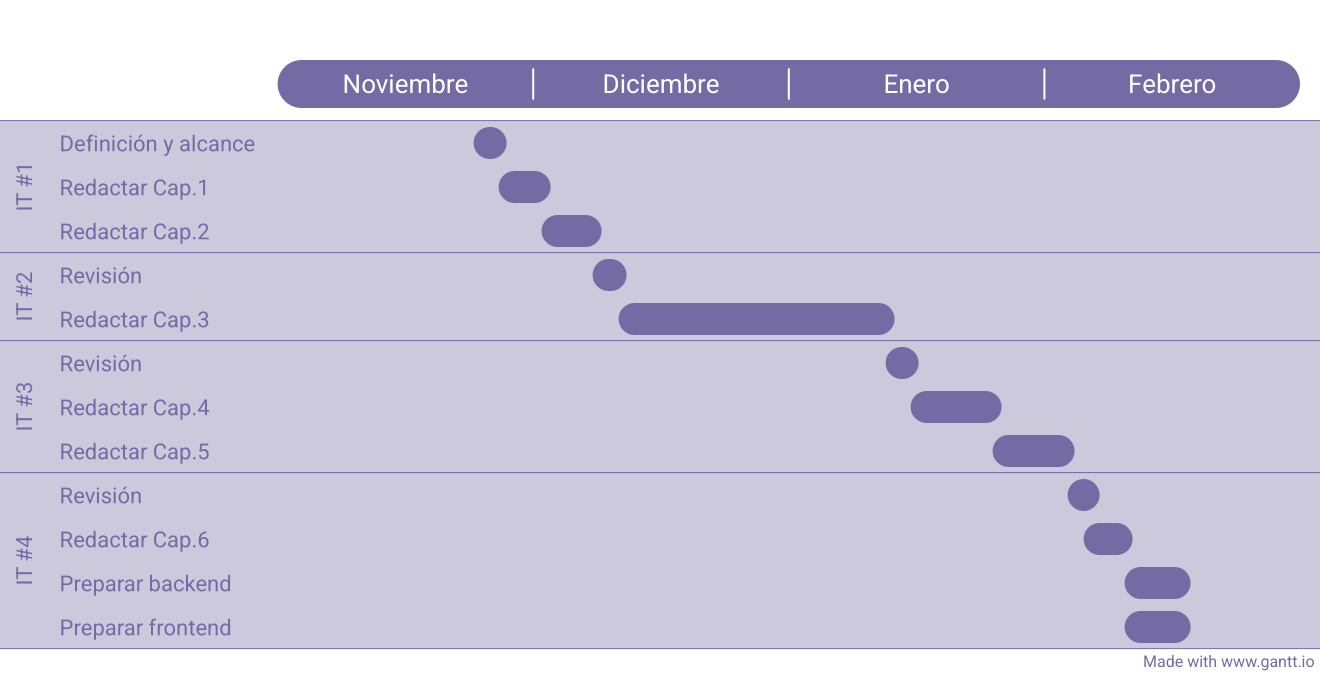
\includegraphics[width=1\textwidth]{imagenes/c4/gantt1.png}}
    \caption{Diagrama de Gantt de los cuatro primeros Sprints.}
    \label{fig:diagrama_gantt1}
\end{figure}

\begin{figure}[H]

    \centering
    \centerline{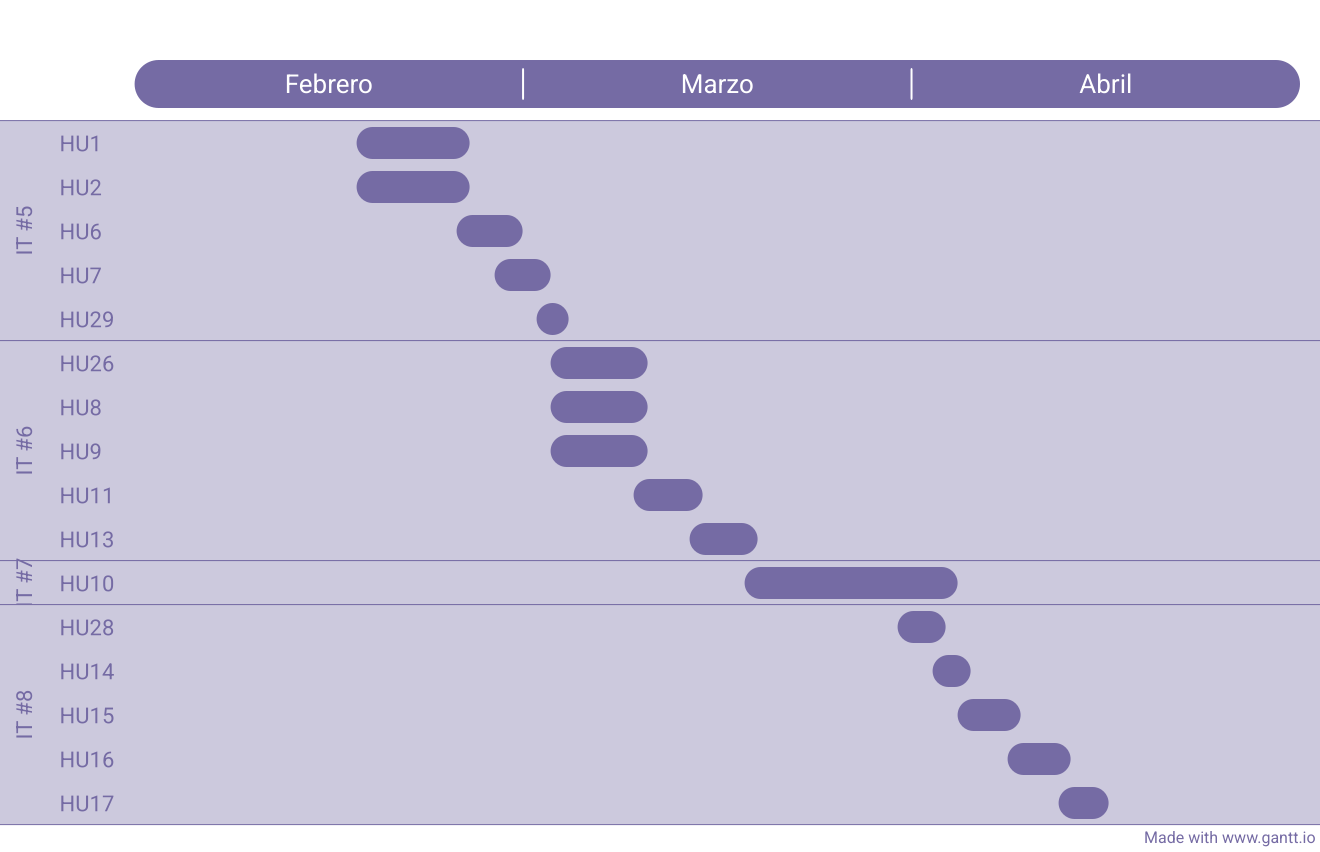
\includegraphics[width=1\textwidth]{imagenes/c4/gantt2.png}}
    \caption{Diagrama de Gantt de los Sprints 5, 6, 7 y 8.}
    \label{fig:diagrama_gantt2}
\end{figure}

\begin{figure}[H]
    \centering
    \centerline{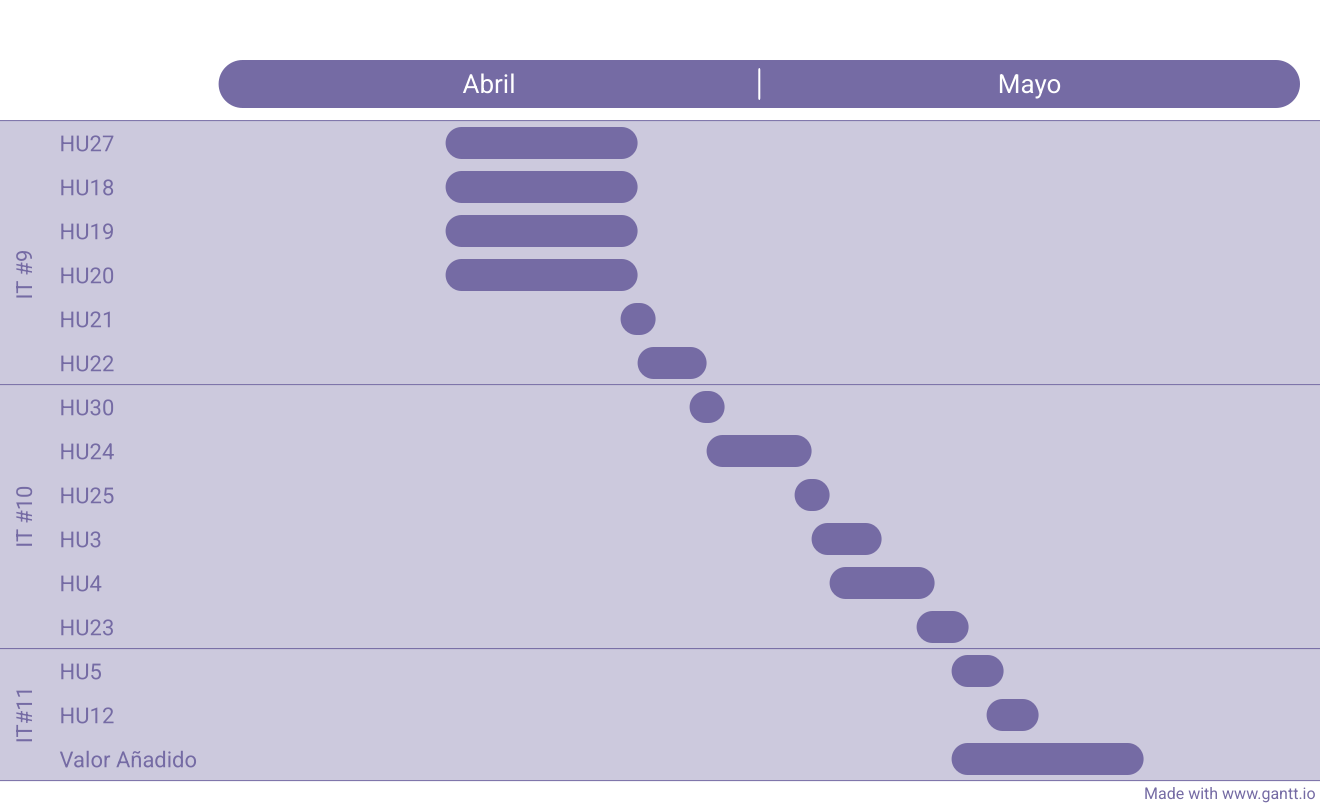
\includegraphics[width=1.1\textwidth]{imagenes/c4/gantt3.png}}
    \caption{Diagrama de Gantt de los Sprints 9, 10 y 11.}
    \label{fig:diagrama_gantt3}
\end{figure}

\begin{figure}[H]
    \centering
    \centerline{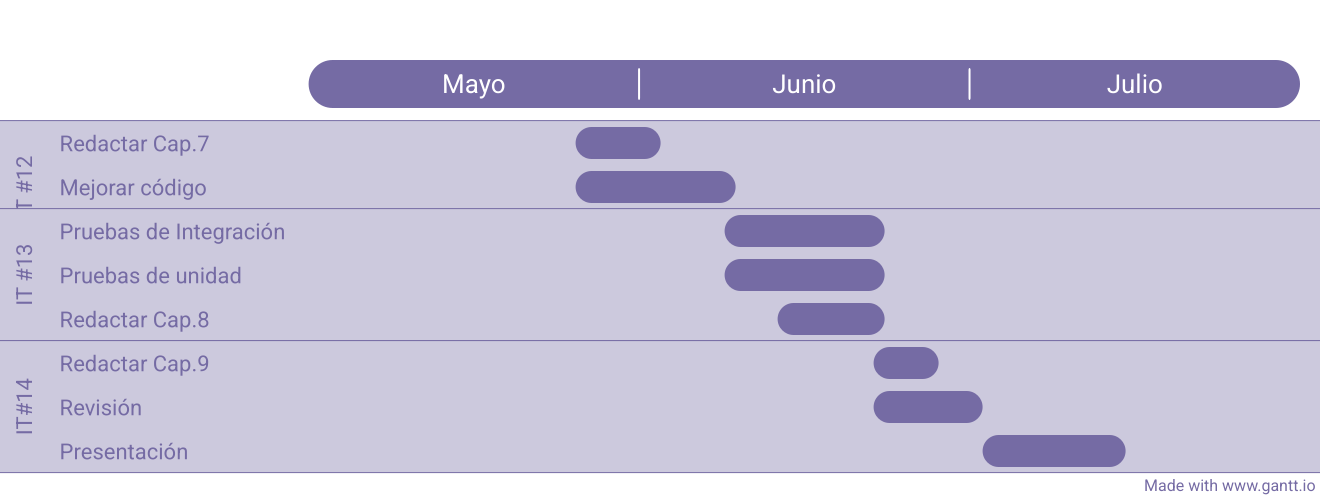
\includegraphics[width=1.2\textwidth]{imagenes/c4/gantt4.png}}
    \caption{Diagrama de Gantt de los Sprints 12, 13 y 14.}
    \label{fig:diagrama_gantt4}
\end{figure}


   \chapter{Análisis del problema}


\section{Historias de Usuario}

\begin{table}[h]
    \centering
    \resizebox{\textwidth}{!}{%
        \begin{tabular}{|
                >{\columncolor[HTML]{D8D8D8}}l |l|
                >{\columncolor[HTML]{D8D8D8}}l |l|l|l|}
            \hline
            \textbf{ID}                                                                  & HU1                                                                                                                                                                                                                                      & \textbf{Nombre}       & \multicolumn{3}{l|}{\begin{tabular}[c]{@{}l@{}}Como usuario quiero registrarme en la aplicación para poder comenzar \\ a utilizar sus funcionalidades.\end{tabular}}                                                                                                                                                                                                \\ \hline
            \textbf{PH}                                                                  & 1                                                                                                                                                                                                                                        & \textbf{Descripcion}  & \multicolumn{3}{l|}{\begin{tabular}[c]{@{}l@{}}El usuario podrá registrarse en el sistema rellenando un formulario con campos \\ como el nombre de usuario, el correo electrónico, la contraseña... \end{tabular}}                                                                                                                                                  \\ \hline
            \textbf{Prioridad}                                                           & 1                                                                                                                                                                                                                                        & \textbf{Dependencias} & \begin{tabular}[c]{@{}l@{}} --- \end{tabular}                                                                                                                                                                      & \cellcolor[HTML]{D8D8D8}\begin{tabular}[c]{@{}l@{}}\textbf{Requisitos Funcionales}\end{tabular} & \begin{tabular}[c]{@{}l@{}}RF 1\end{tabular} \\ \hline
            \multicolumn{3}{|l|}{\cellcolor[HTML]{D8D8D8}\textbf{Pruebas de aceptacion}} & \multicolumn{3}{l|}{\begin{tabular}[c]{@{}l@{}}1. Todos los campos rellenados por el usuario serán almacenados en la \\ base de datos \\ 2. La contraseña se almacenará cifrada para no comprometer la seguridad \\ del usuario \end{tabular}}                                                                                                                                                                                                                                                                                                                                                                                               \\ \hline
        \end{tabular}%
    }
\end{table}


\begin{table}[h]
    \centering
    \resizebox{\textwidth}{!}{%
        \begin{tabular}{|
                >{\columncolor[HTML]{D8D8D8}}l |l|
                >{\columncolor[HTML]{D8D8D8}}l |l|l|l|}
            \hline
            \textbf{ID}                                                                  & HU2                                                                                                                                                                                                                                      & \textbf{Nombre}       & \multicolumn{3}{l|}{\begin{tabular}[c]{@{}l@{}}Como usuario quiero iniciar sesión en la aplicación para poder \\ acceder a sus funcionalidades.\end{tabular}}                                                                                                                                                                                                \\ \hline
            \textbf{PH}                                                                  & 1                                                                                                                                                                                                                                        & \textbf{Descripcion}  & \multicolumn{3}{l|}{\begin{tabular}[c]{@{}l@{}}El usuario podrá registrarse en el sistema rellenando un formulario con campos \\ como el nombre de usuario, el correo electrónico, la contraseña... \end{tabular}}                                                                                                                                                  \\ \hline
            \textbf{Prioridad}                                                           & 1                                                                                                                                                                                                                                        & \textbf{Dependencias} & \begin{tabular}[c]{@{}l@{}} --- \end{tabular}                                                                                                                                                                      & \cellcolor[HTML]{D8D8D8}\begin{tabular}[c]{@{}l@{}}\textbf{Requisitos Funcionales}\end{tabular} & \begin{tabular}[c]{@{}l@{}}RF 1\end{tabular} \\ \hline
            \multicolumn{3}{|l|}{\cellcolor[HTML]{D8D8D8}\textbf{Pruebas de aceptacion}} & \multicolumn{3}{l|}{\begin{tabular}[c]{@{}l@{}}1. Todos los campos rellenados por el usuario serán almacenados en la base de datos \\ 2. La contraseña se almacenará cifrada para no comprometer la seguridad del usuario \end{tabular}}                                                                                                                                                                                                                                                                                                                                                                                               \\ \hline
        \end{tabular}%
    }
\end{table}


\begin{table}[h]
    \centering
    \resizebox{\textwidth}{!}{%
        \begin{tabular}{|
                >{\columncolor[HTML]{D8D8D8}}l |l|
                >{\columncolor[HTML]{D8D8D8}}l |l|l|l|}
            \hline
            \textbf{ID}                                                                  & HU1                                                                                                                                                                                                                                      & \textbf{Nombre}       & \multicolumn{3}{l|}{\begin{tabular}[c]{@{}l@{}}Como usuario quiero registrarme en la aplicación para poder comenzar a utilizar \\ sus funcionalidades.\end{tabular}}                                                                                                                                                                                                \\ \hline
            \textbf{PH}                                                                  & 1                                                                                                                                                                                                                                        & \textbf{Descripcion}  & \multicolumn{3}{l|}{\begin{tabular}[c]{@{}l@{}}El usuario podrá registrarse en el sistema rellenando un formulario con campos \\ como el nombre de usuario, el correo electrónico, la contraseña... \end{tabular}}                                                                                                                                                  \\ \hline
            \textbf{Prioridad}                                                           & 1                                                                                                                                                                                                                                        & \textbf{Dependencias} & \begin{tabular}[c]{@{}l@{}} --- \end{tabular}                                                                                                                                                                      & \cellcolor[HTML]{D8D8D8}\begin{tabular}[c]{@{}l@{}}\textbf{Requisitos Funcionales}\end{tabular} & \begin{tabular}[c]{@{}l@{}}RF 1\end{tabular} \\ \hline
            \multicolumn{3}{|l|}{\cellcolor[HTML]{D8D8D8}\textbf{Pruebas de aceptacion}} & \multicolumn{3}{l|}{\begin{tabular}[c]{@{}l@{}}1. Todos los campos rellenados por el usuario serán almacenados en la base de datos \\ 2. La contraseña se almacenará cifrada para no comprometer la seguridad del usuario \end{tabular}}                                                                                                                                                                                                                                                                                                                                                                                               \\ \hline
        \end{tabular}%
    }
\end{table}


\begin{table}[h]
    \centering
    \resizebox{\textwidth}{!}{%
        \begin{tabular}{|
                >{\columncolor[HTML]{D8D8D8}}l |l|
                >{\columncolor[HTML]{D8D8D8}}l |l|l|l|}
            \hline
            \textbf{ID}                                                                  & HU1                                                                                                                                                                                                                                      & \textbf{Nombre}       & \multicolumn{3}{l|}{\begin{tabular}[c]{@{}l@{}}Como usuario quiero registrarme en la aplicación para poder comenzar a utilizar \\ sus funcionalidades.\end{tabular}}                                                                                                                                                                                                \\ \hline
            \textbf{PH}                                                                  & 1                                                                                                                                                                                                                                        & \textbf{Descripcion}  & \multicolumn{3}{l|}{\begin{tabular}[c]{@{}l@{}}El usuario podrá registrarse en el sistema rellenando un formulario con campos \\ como el nombre de usuario, el correo electrónico, la contraseña... \end{tabular}}                                                                                                                                                  \\ \hline
            \textbf{Prioridad}                                                           & 1                                                                                                                                                                                                                                        & \textbf{Dependencias} & \begin{tabular}[c]{@{}l@{}} --- \end{tabular}                                                                                                                                                                      & \cellcolor[HTML]{D8D8D8}\begin{tabular}[c]{@{}l@{}}\textbf{Requisitos Funcionales}\end{tabular} & \begin{tabular}[c]{@{}l@{}}RF 1\end{tabular} \\ \hline
            \multicolumn{3}{|l|}{\cellcolor[HTML]{D8D8D8}\textbf{Pruebas de aceptacion}} & \multicolumn{3}{l|}{\begin{tabular}[c]{@{}l@{}}1. Todos los campos rellenados por el usuario serán almacenados en la base de datos \\ 2. La contraseña se almacenará cifrada para no comprometer la seguridad del usuario \end{tabular}}                                                                                                                                                                                                                                                                                                                                                                                               \\ \hline
        \end{tabular}%
    }
\end{table}


\begin{table}[h]
    \centering
    \resizebox{\textwidth}{!}{%
        \begin{tabular}{|
                >{\columncolor[HTML]{D8D8D8}}l |l|
                >{\columncolor[HTML]{D8D8D8}}l |l|l|l|}
            \hline
            \textbf{ID}                                                                  & HU1                                                                                                                                                                                                                                      & \textbf{Nombre}       & \multicolumn{3}{l|}{\begin{tabular}[c]{@{}l@{}}Como usuario quiero registrarme en la aplicación para poder comenzar a utilizar \\ sus funcionalidades.\end{tabular}}                                                                                                                                                                                                \\ \hline
            \textbf{PH}                                                                  & 1                                                                                                                                                                                                                                        & \textbf{Descripcion}  & \multicolumn{3}{l|}{\begin{tabular}[c]{@{}l@{}}El usuario podrá registrarse en el sistema rellenando un formulario con campos \\ como el nombre de usuario, el correo electrónico, la contraseña... \end{tabular}}                                                                                                                                                  \\ \hline
            \textbf{Prioridad}                                                           & 1                                                                                                                                                                                                                                        & \textbf{Dependencias} & \begin{tabular}[c]{@{}l@{}} --- \end{tabular}                                                                                                                                                                      & \cellcolor[HTML]{D8D8D8}\begin{tabular}[c]{@{}l@{}}\textbf{Requisitos Funcionales}\end{tabular} & \begin{tabular}[c]{@{}l@{}}RF 1\end{tabular} \\ \hline
            \multicolumn{3}{|l|}{\cellcolor[HTML]{D8D8D8}\textbf{Pruebas de aceptacion}} & \multicolumn{3}{l|}{\begin{tabular}[c]{@{}l@{}}1. Todos los campos rellenados por el usuario serán almacenados en la base de datos \\ 2. La contraseña se almacenará cifrada para no comprometer la seguridad del usuario \end{tabular}}                                                                                                                                                                                                                                                                                                                                                                                               \\ \hline
        \end{tabular}%
    }
\end{table}


\begin{table}[h]
    \centering
    \resizebox{\textwidth}{!}{%
        \begin{tabular}{|
                >{\columncolor[HTML]{D8D8D8}}l |l|
                >{\columncolor[HTML]{D8D8D8}}l |l|l|l|}
            \hline
            \textbf{ID}                                                                  & HU1                                                                                                                                                                                                                                      & \textbf{Nombre}       & \multicolumn{3}{l|}{\begin{tabular}[c]{@{}l@{}}Como usuario quiero registrarme en la aplicación para poder comenzar a utilizar \\ sus funcionalidades.\end{tabular}}                                                                                                                                                                                                \\ \hline
            \textbf{PH}                                                                  & 1                                                                                                                                                                                                                                        & \textbf{Descripcion}  & \multicolumn{3}{l|}{\begin{tabular}[c]{@{}l@{}}El usuario podrá registrarse en el sistema rellenando un formulario con campos \\ como el nombre de usuario, el correo electrónico, la contraseña... \end{tabular}}                                                                                                                                                  \\ \hline
            \textbf{Prioridad}                                                           & 1                                                                                                                                                                                                                                        & \textbf{Dependencias} & \begin{tabular}[c]{@{}l@{}} --- \end{tabular}                                                                                                                                                                      & \cellcolor[HTML]{D8D8D8}\begin{tabular}[c]{@{}l@{}}\textbf{Requisitos Funcionales}\end{tabular} & \begin{tabular}[c]{@{}l@{}}RF 1\end{tabular} \\ \hline
            \multicolumn{3}{|l|}{\cellcolor[HTML]{D8D8D8}\textbf{Pruebas de aceptacion}} & \multicolumn{3}{l|}{\begin{tabular}[c]{@{}l@{}}1. Todos los campos rellenados por el usuario serán almacenados en la base de datos \\ 2. La contraseña se almacenará cifrada para no comprometer la seguridad del usuario \end{tabular}}                                                                                                                                                                                                                                                                                                                                                                                               \\ \hline
        \end{tabular}%
    }
\end{table}
\section{Diagrama de Clases}

   
   \input{capitulos/06_Diseño}
   
   \chapter{Implementación}
En este séptimo capítulo se detallará la implementación del sistema. En primer lugar,  se presentará la estructura del proyecto que se ha realizado para el frontend y del backend y, a continuación,
se describirá la implementación de cada una de las funcionalidades del sistema, presentando la documentación de cada ruta de la API y describiendo el código escrito durante el desarrollo.

\section{Herramientas utilizadas}
En el desarrollo de la aplicación se utilizarán varias herramientas externas que ayudarán en el cumplimiento de los objetivos y facilitarán la implementación de cada una de las historias de usuario. A continuación se muestran algunas
de ellas:

\subsection{Git \& Github}
Git es una herramienta para el control de versiones. Nos permitirá mantener un historial de cambios que nos ayudarán en la implementación cuando necesitemos "volver atrás", así como poder trabajar en distintas ramas cuando la situación lo requiera (por ejemplo, si encontramos un error puedo abrir una nueva rama para poder trabajar exclusivamente en arreglarlo).

Como complemento a Git, usaremos Github, una plataforma para alojar repositorios de Git. En Github tendremos un repositorio para el frontend y para el backend, donde se irán subiendo los cambios que se vayan realizando. Esto facilitará la posibilidad de trabajar en el desarrollo en varios dispositivos permitiendo un desarrollo más flexible en cuanto a en qué dispositivo y cuándo trabajar. 

\subsection{Jira}
Jira es una herramienta para la gestión de proyectos. Usaré Jira para facilitar el cumplimiento de algunos de los principios de metodologías ágiles que usamos en la planificación y controlar el seguimiento de esta última. En Jira tendré un Sprint Backlog, cuyas historias de usuario y tareas irán moviéndose a los distintos Sprints para su desarrollo.

\begin{figure}[H]
  \centering
  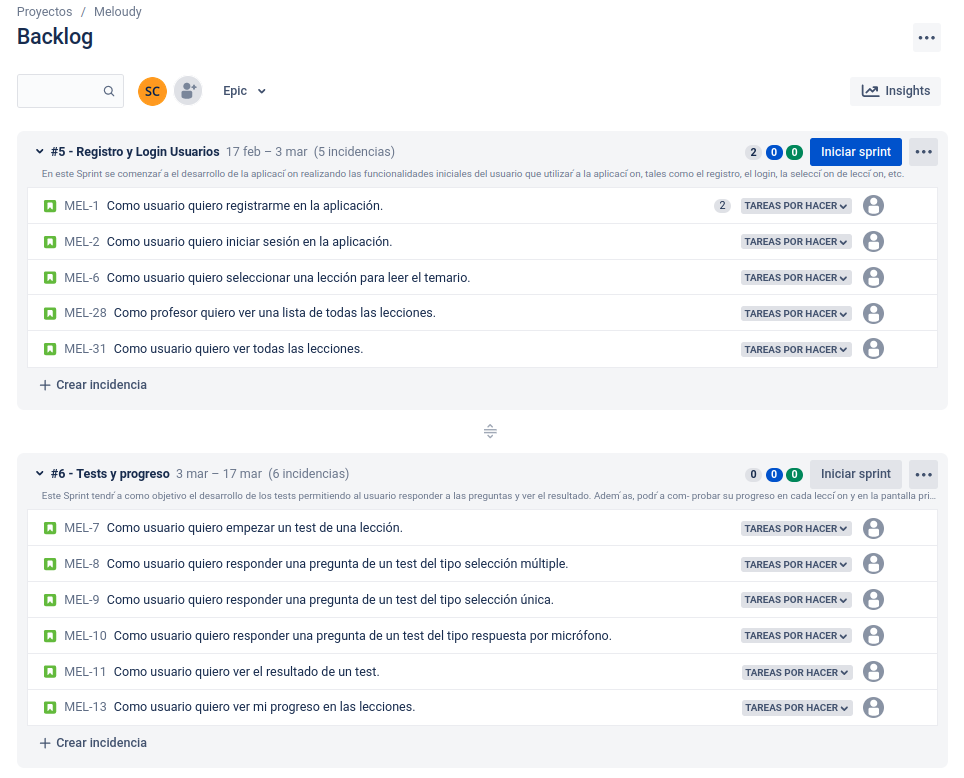
\includegraphics[width=\textwidth]{imagenes/c7/jira.png}
  \caption{Captura de pantalla de Jira. En ella se puede ver el Sprint Backlog, donde se encuentran las historias de usuario repartidas entre los sprints.}
  \label{fig:login}
\end{figure}


\subsection{Visual Studio Code \& Android Studio}
Visual Studio Code es el editor de código fuente que se usará para implementar la parte backend (NodeJS) de nuestro sistema. Nos permitirá un desarrollo más cómodo y eficiente, ya que nos ofrece una gran variedad de herramientas para el desarrollo, como la posibilidad de depurar el código, herramientas para el formato de los distintos lenguajes de programación, visualizador de versiones de Git, etc.

Android Studio es el entorno de desarrollo integrado oficial para la plataforma Android. Se utilizará para implementar la parte de frontend (flutter) y para ejecutar la aplicación en un simulador de Android o en nuestro propio dispositivo físico.

\subsection{Mongo Compass}
Mongo Compass es una herramienta interactiva para la consulta, la gestión y el análisis de los datos en MongoDB. Se utilizará para comprobar si las consultas se realizan correctamente y para añadir datos a la base de datos (lecciones, preguntas...) de forma fácil, cómoda y rápida.

\begin{figure}[H]
  \centering
  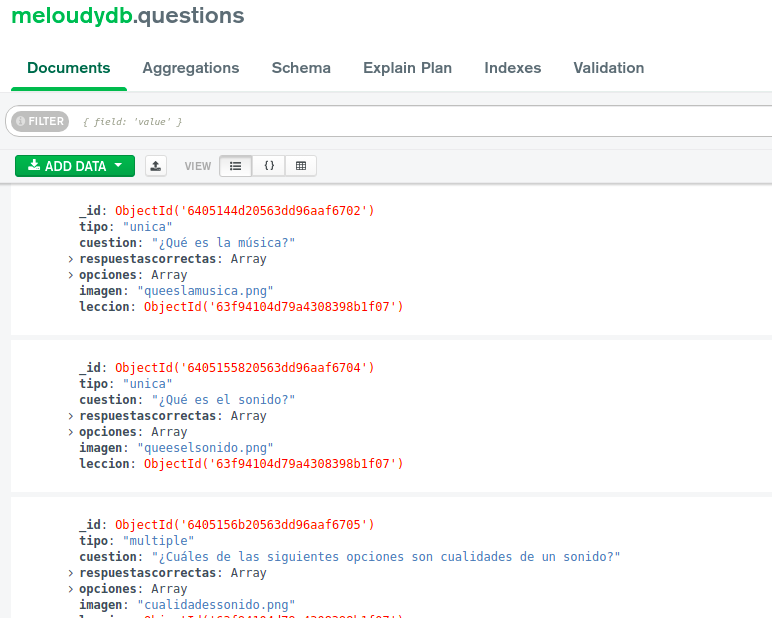
\includegraphics[width=\textwidth]{imagenes/c7/compass.png}
  \caption{Captura de pantalla de Jira. En ella se puede ver el Sprint Backlog, donde se encuentran las historias de usuario repartidas entre los sprints.}
  \label{fig:login}
\end{figure}

\subsection{Postman}
Postman es una plataforma API para diseñar, construir, probar e iterar APIs. Se utilizará en la implementación de nuestra aplicación para comprobar el funcionamiento de las rutas especificadas y codificadas en el backend. Además, podremos realizar una documentación de nuestra API mediante
esta herramienta para facilitar la comprensión y el mantenimiento de cada ruta.



\section{Estructura del proyecto}
\label{sec:estructura}
Como se mencionó en la arquitectura del sistema en el anterior capítulo, el proyecto se ha desarrollado en dos partes, una parte de frontend y otra de backend. La parte de frontend se ha desarrollado en Flutter y la parte de backend se ha desarrollado en Node.js. 

La estructura del proyecto se puede ver en la siguiente imagen:
\begin{figure}[H]
  \centering
  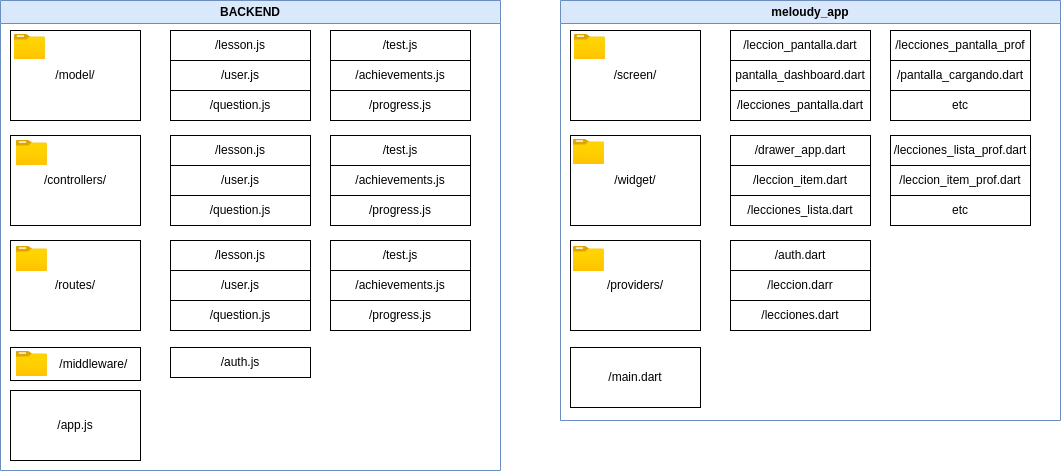
\includegraphics[width=\textwidth]{imagenes/c7/estructura.png}
  \caption{Estructura del proyecto, donde se puede ver la parte de frontend y la parte de backend.}
  \label{fig:login}
\end{figure}

En la figura anterior podemos ver que el desarrollo del proyecto se ha realizado en dos partes, una parte de frontend y otra de backend.

La parte de backend se ha desarrollado en Node.js, por lo que se han dividido los archivos en carpetas de acuerdo a su funcionalidad:
\begin{itemize}
    \item \textit{app.js}: Archivo principal de la aplicación. En él se configura el servidor y se importan las rutas.
    \item \textit{routes}: Carpeta que contiene las rutas de la API. Dentro se encuentran distintos archivos que contienen las rutas de cada entidad de la base de datos (user, lesson, question...).
    \item \textit{controllers}: Carpeta que contiene los controladores de las rutas de la API. Dentro se encuentran distintos archivos que contienen los controladores de cada entidad de la base de datos (user, lesson, question...)
    \item \textit{models}: Carpeta que contiene los modelos de la base de datos.
    \item \textit{middleware}: Carpeta que contiene los middleware de la aplicación. Por dichos middleware pasarán algunas peticiones que se hagan a la API.
\end{itemize}

La parte de frontend se ha desarrollado en Flutter, por lo que se han dividido los archivos en carpetas de acuerdo a su funcionalidad, dentro de la carpeta \textit{lib}:

\begin{itemize}
  \item \textit{main.dart}: Archivo principal de la aplicación. En él se configura la aplicación y se importan las rutas.
  \item \textit{providers}: Carpeta que contiene los providers de la aplicación. Los providers son clases que se encargan de gestionar el estado de la aplicación.
  \item \textit{screen}: Carpeta que contiene las pantallas de la aplicación. Dentro se encuentran distintos archivos que implementan cada pantalla de la aplicación.
  \item \textit{widgets}: Carpeta que contiene los widgets de la aplicación. Dentro se encuentran los archivos de los widgets que se utilizan en las distintas pantallas de la aplicación.
\end{itemize}

\section{Definición de la API (Backend)}
\label{sec:api}
En esta sección se describirá la API que se ha desarrollado para el sistema. La API se ha desarrollado en Node.js y se ha utilizado el framework Express para trabajar con el protocolo HTTP.

\subsection{Rutas}

\subsubsection{Usuarios}
\label{sec:usuarios}
La API cuenta con las siguientes rutas para la gestión de usuarios:

\begin{itemize}
    \item \textit{POST /api/user/registro}: Ruta para registrar un usuario. Recibe los datos del usuario en el cuerpo de la petición, encripta la contraseña y almacena todos los datos en la base de datos. Si el usuario se registra correctamente, se devuelve un token que se utilizará para la autenticación de las peticiones que se hagan a la API.
    \item \textit{POST /api/user/login}: Ruta para iniciar sesión. Recibe los datos del usuario en el cuerpo de la petición y comprueba si el usuario existe en la base de datos. En caso de que el usuario exista, se comprueba que la contraseña sea correcta. Si la contraseña es correcta, se devuelve un token que se utilizará para la autenticación de las peticiones que se hagan a la API.
    \item \textit{GET /api/user/get-user/\{id\}}: Ruta para obtener los datos de un usuario. Recibe por parámetro el id del usuario y devuelve los datos de dicho usuario.
    \item \textit{GET /api/user/get-users}: Ruta para obtener los datos de todos los usuarios. No recibe ningún parámetro y devuelve una lista de los datos de todos los usuarios.
%    \item \textit{PUT /api/user}: Ruta para actualizar los datos de un usuario. Recibe los datos del usuario en el cuerpo de la petición y los actualiza en la base de datos. Si el usuario se actualiza correctamente, se devuelve un token que se utilizará para la autenticación de las peticiones que se hagan a la API.
    \item \textit{DELETE /api/user/delete-user/\{id\}}: Ruta para eliminar un usuario. Recibe por parámetro el id del usuario y lo elimina de la base de datos.
    
\end{itemize}

\subsubsection{Lecciones}
\label{sec:lecciones}
La API cuenta con las siguientes rutas para la gestión de lecciones:

\begin{itemize}
    \item \textit{POST /api/lesson/create-lesson}: Ruta para crear una lección. Recibe los datos de la lección en el cuerpo de la petición y los almacena en la base de datos. Si la lección se crea correctamente, se devuelve la lección creada.
    \item \textit{GET /api/lesson/get-lessons/\{id\}}: Ruta para obtener los datos de una lección. Recibe por parámetro el id de la lección y se devuelven los datos de esta.
    \item \textit{PUT /api/lessons/:id}: Ruta para actualizar los datos de una lección. Recibe los datos de la lección en el cuerpo de la petición y los actualiza en la base de datos. Si la lección se actualiza correctamente, se devuelve la lección actualizada.
    \item \textit{DELETE /api/lessons/:id}: Ruta para eliminar una lección. Recibe el token del usuario en el encabezado de la petición y comprueba si el token es correcto. Si el token es correcto, se elimina de la base de datos la lección cuyo id coincida con el recibido.
    \item \textit{POST /api/lesson/upload-image/}: Ruta para subir una imagen de una lección al servidor. Recibe por parámetro el id de la lección y la imagen en el cuerpo de la petición.
\end{itemize}

\subsubsection{Preguntas}
\label{sec:preguntas}
La API cuenta con las siguientes rutas para la gestión de preguntas:

\begin{itemize}
  \item \textit{GET /api/question/get-questions}: Ruta para obtener todas las preguntas almacenadas en la base de datos.
  \item \textit{GET /api/question/get-questions/\{idLeccion\}}: Ruta para obtener las preguntas de una lección. Recibe por parámetro el id de la lección y devuelve todas las preguntas existentes de dicha lección.
  \item \textit{GET /api/question/get-question-test/\{idTest\}}: Ruta para obtener las preguntas de un test. Recibe por parámetro el id del test y devuelve todas las preguntas existentes de dicho test junto con el propio test.
  \item \textit{GET /api/question/get-question/\{id\}}: Ruta para obtener los datos de una pregunta. Recibe por parámetro el id de la pregunta y devuelve los datos de dicha pregunta.
\end{itemize}

\subsubsection{Tests}
\label{sec:tests}
La API cuenta con las siguientes rutas para la gestión de tests:

\begin{itemize}
  \item \textit{GET /api/progress/get-tests-progress/\{idUsuario\}/\{idLeccion\}}: Ruta para obtener todos los tests de un usuario en una lección. Recibe por parámetro el id del usuario y el de la lección, busca el progreso a partir de estos identificadores, busca todos los tests de dicho progreso y los devuelve.
\end{itemize}


\subsubsection{Progress}
\label{sec:progress}
La API cuenta con las siguientes rutas para la gestión del progreso de los usuarios:

\begin{itemize}
  \item \textit{POST /api/progress/create-test-and-progress/}: Ruta para crear un test y el progreso de un usuario. Recibe los datos del test y del progreso en el cuerpo de la petición y los almacena en la base de datos. Si el progreso ya estaba creado, solamente se almacena el nuevo test y se añade a la lista de tests del progreso. Si el test y el progreso se crean correctamente, se devuelve el test y el progreso creados. 
\end{itemize}




\subsection{Middleware}
\label{sec:middleware}
Un middleware es una función intermediaria que se utiliza para realizar acciones comunes a varias funcionalidades. La API cuenta con los siguientes middleware:

\begin{itemize}
  \item \textit{auth}: Middleware que comprueba si el token del usuario es correcto (es decir, si el usuario está identificado en la aplicación). Si el token es correcto, se pasa a la siguiente función. Si el token no es correcto, se devuelve un error.
%  \item \textit{authAdmin}: Middleware que comprueba si el token del usuario es correcto y si el usuario es administrador. Si el token es correcto y el usuario es administrador, se pasa a la siguiente función. Si el token no es correcto o el usuario no es administrador, se devuelve un error.
\end {itemize}

\newpage
\section{Funcionalidad de inicio}
\label{sec:inicio}
A continuación presentamos la funcionalidad básica de la aplicación que usará cualquier usuario que se registre:


% \subsection{Pantallas y Widgets básicos}
% \label{sec:widgets}
% La aplicación cuenta con una serie de pantallas y widgets que se utilizan en todas las pantallas de la aplicación. 
% Estos widgets se han desarrollado para que se puedan reutilizar en las distintas pantallas de la aplicación. A continuación se describen los widgets y pantallas que se han desarrollado:


\subsection{Drawer}
Un drawer es un menú lateral que se puede abrir y cerrar y que se utiliza para acceder a distintas pantallas de la aplicación. En este caso, se
abre y se cierra clickando en el icono superior izquierdo de la aplicación. Se ha utilizado el llamado "menú hamburguesa". En la siguiente imagen se puede ver el drawer abierto:

\begin{figure}[H]
    \centering
    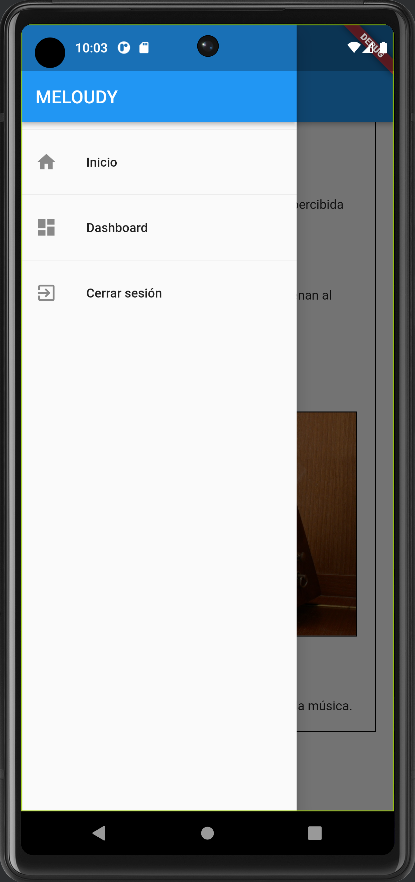
\includegraphics[width=0.4\textwidth]{imagenes/c7/drawer.png}
    \caption{Drawer abierto en la aplicación con tres opciones (por ser desde la vista del profesor): Inicio, Dashboard y Cerrar sesión.}
    \label{fig:drawer}
\end{figure}


\subsection{Sesión}
\label{sec:sesion}
Se han desarrollado tres características adicionales relacionadas con la sesión de usuario y que explicaremos con más detalle en cada uno de los apartados de la sesión.
\begin{itemize}
    \item \textbf{Encriptación de la contraseña:} La contraseña del usuario se encripta antes de ser almacenada en la base de datos para evitar que sea visible por cualquier persona que tenga acceso a esta. De esta forma
    garantizamos que se cumple el requisito de seguridad de la contraseña. Para esto se ha utilizado un algoritmo hash de la biblioteca \textit{bcrypt}.
    El diagrama que explica el proceso de encriptación se muestra en la siguiente imagen:
    \begin{figure}[H]
      \centering
      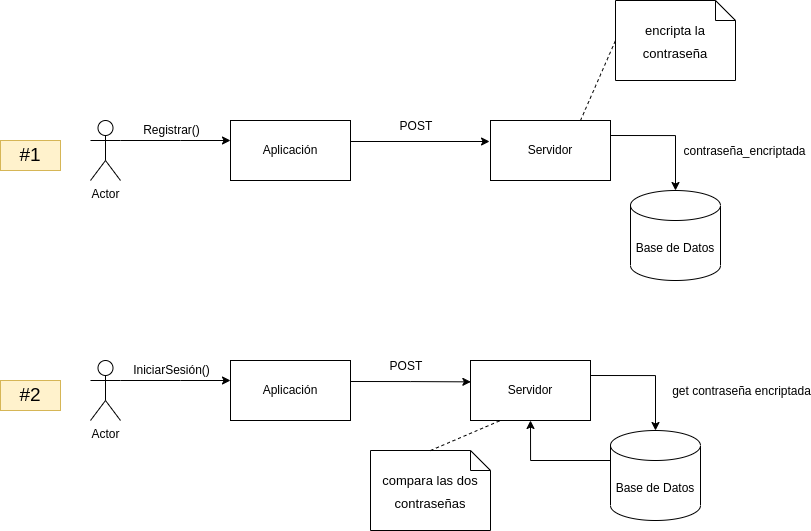
\includegraphics[width=0.9\textwidth]{imagenes/c7/logindiag.png}
      \caption{Diagrama que explica el proceso de encriptación en el inicio de sesión desarrollado en la aplicación.}
      \label{fig:login}
    \end{figure}

    \item \textbf{Intercambio de token:} El servidor proporciona un token al usuario cuando se registra o inicia sesión. Este token se añade a las peticiones que se hagan a la API. De esta forma, garantizamos que se cumple el requisito de seguridad de la sesión y 
    que todas las peticiones válidas que se hagan a la API son de usuarios registrados. Además, el token fija una fecha de expiración al crearse para aumentar la seguridad del usuario. Esta funcionalidad se ha logrado con el paquete \textit{jsonwebtoken} de NodeJS.
    El diagrama que explica el proceso de intercambio de token se muestra en la siguiente imagen:

    \begin{figure}[H]
      \centering
      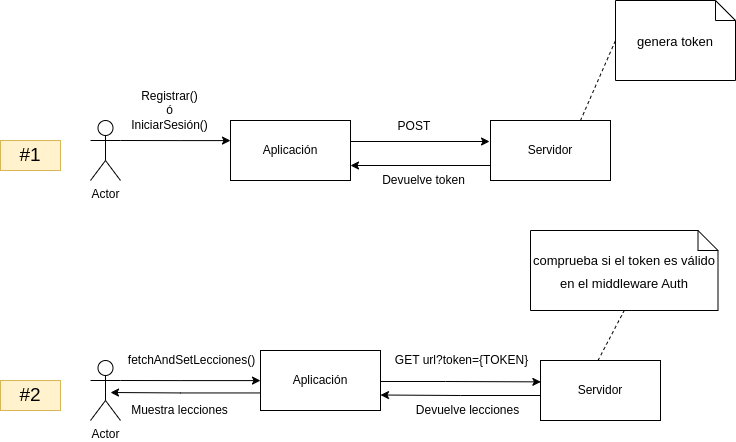
\includegraphics[width=0.9\textwidth]{imagenes/c7/tokendiag.png}
      \caption{Diagrama que explica el proceso de intercambio de token en el inicio de sesión desarrollado en la aplicación.}
      \label{fig:token}
    \end{figure}

    \item \textbf{Sesión entre instancias:} La sesión se mantiene entre instancias de la aplicación. Es decir, si el usuario cierra la aplicación y la vuelve a abrir, no tendrá que volver a iniciar sesión si no ha cerrado la sesión o si el token no ha expirado. 
    Esto se ha conseguido mediante el almacenamiento del token en la memoria local del dispositivo con la biblioteca \textit{shared\_preferences}. De esta forma, cuando el usuario inicia sesión, el token se almacena en el almacenamiento local del dispositivo 
    y cuando el usuario cierra la aplicación y la vuelve a abrir, el token se recupera del almacenamiento local del dispositivo y se comprueba si es correcto. Si es correcto, se pasa a la siguiente pantalla. Si no es correcto, se vuelve a la pantalla de inicio de sesión.
    Este token además estará siendo comprobado constantemente para que si el este expira, se cierre la sesión y se vuelva a la pantalla de inicio de sesión evitando accesos no autorizados.

    El diagrama que explica el proceso de sesión entre instancias se muestra en la siguiente imagen:

    \begin{figure}[H]
      \centering
      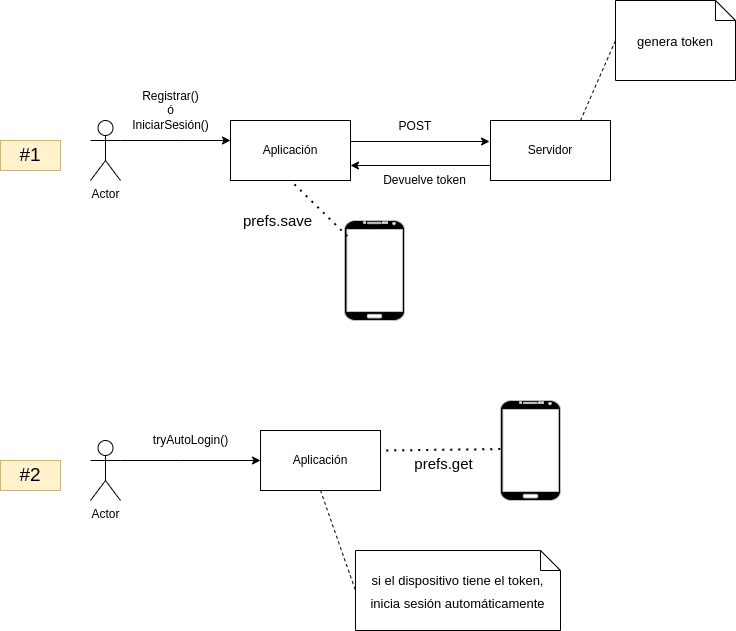
\includegraphics[width=0.9\textwidth]{imagenes/c7/token2.png}
      \caption{Diagrama que explica el proceso de sesión entre instancias en el inicio de sesión desarrollado en la aplicación.}
      \label{fig:sesion}

    \end{figure}

  \end{itemize}

\subsubsection{Inicio de sesión}
\textit{Desarrollado en el Sprint 5}
\label{sec:login}

La aplicación cuenta con una pantalla de inicio de sesión para que los usuarios puedan acceder a la aplicación con su cuenta registrada previamente. 
Para el inicio de sesión, el usuario deberá introducir su nombre de usuario y su contraseña. Si el usuario no tiene una cuenta, podrá registrarse pulsando en el botón 'Registrarse'. En la siguiente imagen se puede ver la pantalla de inicio de sesión:

\begin{figure}[H]%
  \centering
  \subfloat[\centering Pantalla de login]{{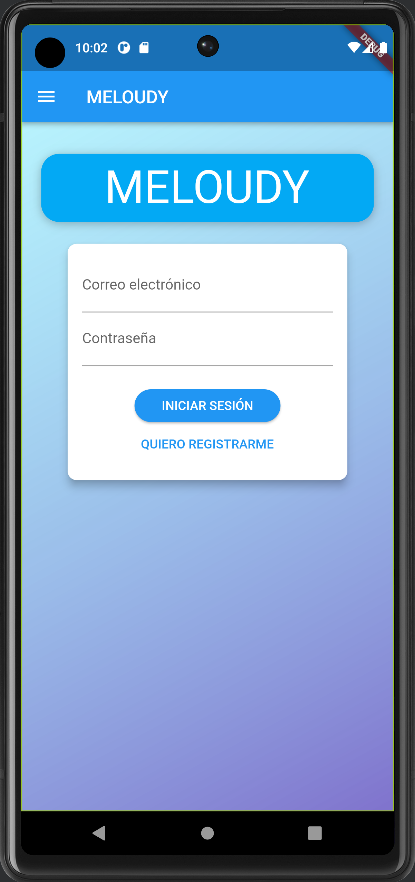
\includegraphics[width=0.40\textwidth]{imagenes/c7/login.png} }}%
  \qquad
  \subfloat[\centering Estructura en componentes de la pantalla de login.]{{ 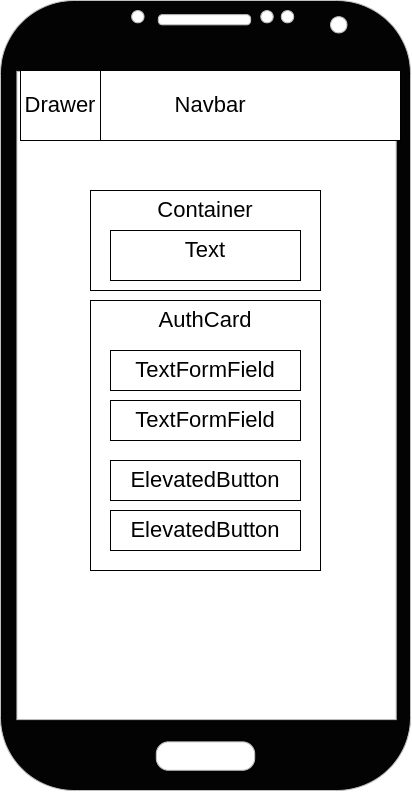
\includegraphics[width=0.406\textwidth]{imagenes/c7/logincompo.png} }}%
  \caption{Pantalla de inicio de sesión del usuario donde se puede ver el formulario de inicio de sesión con los campos de usuario (correo) y contraseña.}%
  \label{fig:login}%
\end{figure}


\paragraph*{Vista}
Empezando por la vista, se ha desarrollado un widget para la pantalla de inicio de sesión. Este widget se compone de un formulario con dos campos de texto, uno para el nombre de usuario y otro para la contraseña. Además, el formulario contiene un botón para iniciar sesión y otro para ir a registrarse si el usuario así lo desea.

La pantalla tiene una pila que contiene dos widgets: un container con un fondo en degradado conseguido con el atributo \textit{gradient} de la clase \textit{BoxDecoration} de Flutter, y un SingleChildScrollView que consta de un widget Column para poder colocar los elementos de forma vertical. Dichos elementos son: un \textit{Container} para el título de la aplicación y un Widget personalizado que contiene el formulario de inicio de sesión \textit{AuthCard()}.
Este último no es más que un widget de la clase \textit{Card} con dos \textit{TextFormField} (uno para el correo electrónico y otro para la contraseña) y un \textit{ElevatedButton} para proceder al inicio de sesión.

\paragraph*{Lógica}
En cuanto a la lógica, una vez el cliente pulsa el botón de 'Iniciar sesión', se llama a la función asíncrona \textit{submit}, la cual se encarga de comprobar que los datos introducidos son correctos.
Cuando los datos son comprobados, se procede a iniciar sesión en la aplicación mediante el método de inicio de sesión del Provider Auth. Para esto, se envia una petición HTTP POST a la ruta \textit{/user/login} de la API con los datos escritos en el formulario de inicio de sesión.

Por otro lado, en el servidor cuando la petición es recibida a dicha ruta, se ejecuta una función en el controlador para el inicio de sesión de usuarios. Esta función capta los valores y comprueba que el usuario existe en la base de datos. Si el usuario existe, se comprueba que la contraseña introducida es correcta mediante el método \textit{verify} de bcrypt. Si los datos son correctos, se genera el token de sesión y se devuelve al cliente. Si el usuario no existe o la contraseña es incorrecta, se devuelve un código de estado 400 y un mensaje de error.

Cuando el cliente recibe la respuesta del servidor, se comprueba si el código de estado es 200, lo que significa que el inicio de sesión ha sido correcto. En este caso, se almacena el token de sesión en el dispositivo tal y como se ha explica en la sección \ref{sec:sesion}. 
\newpage
\subsubsection{Registro}
\textit{Desarrollado en el Sprint 5}
\label{sec:register}

La aplicación cuenta con una pantalla de registro para que los usuarios puedan registrarse en la aplicación. Para el registro, el usuario deberá introducir su nombre de usuario y su contraseña dos veces. Si el usuario ya tiene una cuenta, podrá iniciar sesión pulsando en el botón 'Iniciar sesión'. En la siguiente imagen se puede ver la pantalla de registro:



\paragraph*{Vista}
La vista del registro es muy similar a la del inicio de sesión. La única diferencia es que el formulario contiene un campo adicional para introducir la contraseña otra vez por razones de seguridad.

\begin{figure}[H]
  \centering
  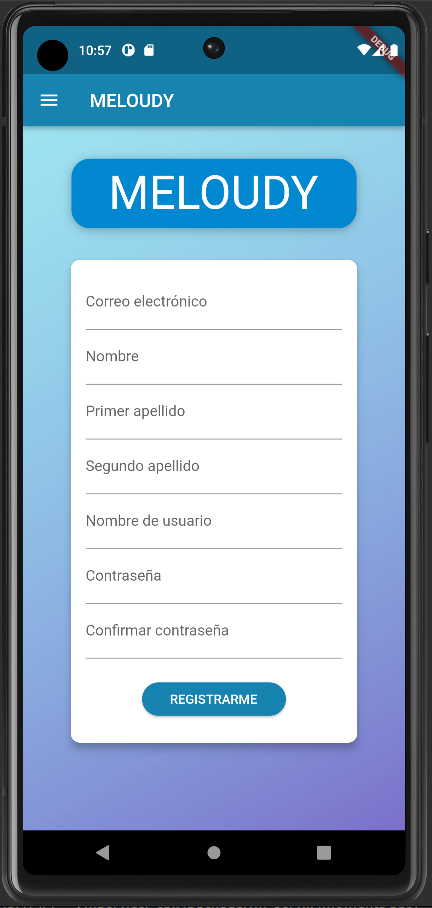
\includegraphics[width=0.4\textwidth]{imagenes/c7/registro.png}
  \caption{Pantalla de registro de los usuarios donde se puede ver el formulario de registro con los campos de usuario (correo), contraseña y repetir la contraseña.}
  \label{fig:register}
\end{figure}


\paragraph*{Lógica}
En cuanto a la lógica, una vez el cliente pulsa el botón de 'Registrarse', también se llama a la función asíncrona \textit{submit}, que se encarga de comprobar que los datos introducidos 
son correctos. Cuando se ha hecho esto, si los datos son válidos, la función llama al método de registro del Provider Auth, el cual envia una petición HTTP POST a la ruta \textit{/user/registro}
 de la API con los datos escritos en el formulario de registro. 

Para poder procesar esta petición de Flutter, una vez el servidor recibe la petición a la ruta de registro, se ejecuta una función en el controlador para el registro de usuarios.
 Esta función capta los valores, encripta la contraseña y crea el usuario en la base de datos. Si los datos son correctos, se genera un token de sesión y
  se devuelve al cliente junto con un código de estado 201 y un mensaje de éxito. Si el registro no es correcto, se devuelve un código de estado 400 y un mensaje de error.

  Cuando Flutter recibe la respuesta del servidor, almacena el token de sesión en el dispositivo tal y como se ha explica en la sección \ref{sec:sesion}.

\subsubsection{Cierre de sesión}
\textit{Desarrollado en el Sprint 5}
\label{sec:logout}

La aplicación cuenta con una opción para cerrar sesión. Para cerrar sesión, el usuario deberá pulsar en el botón \textit{Cerrar sesión} que se encuentra en el drawer (barra lateral) de la aplicación. También se cerrará sesión automáticamente si el token ha expirado.

\paragraph*{Vista}
Para el cierre de sesión, se ha añadido una fila al drawer (barra lateral) de la aplicación, el cual el usuario clicará cuando desee cerrar su sesión.

\paragraph*{Lógica}
La lógica del cierre de sesión es sencilla: se llama a la función \textit{logout} de la clase \textit{Auth} donde se restablecen los valores de la sesión y se limpian los datos de la sesión almacenados en el dispositivo con el paquete \textit{shared\_preferences}. 
Esta limpieza de datos se realiza en el método \textit{clear}.
Además, se ha añadido un timer que se encarga de cerrar la sesión automáticamente si el token ha expirado. Este timer se ejecuta cada cierto tiempo y comprueba si el token ha expirado. Si es así, se llama al método \textit{logout} mencionado anteriormente.

\newpage

\section{Funcionalidad de usuario}
\label{sec:funcionalidad_usuario}


\subsection{Lista de lecciones}
\textit{Desarrollado en el Sprint 5}
\label{sec:lista_lecciones}

La aplicación cuenta con una lista de lecciones que el usuario puede ver. Esta lista es la pantalla inicial de la aplicación y el usuario la visualizará al iniciar sesión. También puede acceder a ella pulsando el botón \textit{Inicio} que se encuentra en el drawer (barra lateral) de la aplicación.


\begin{figure}[H]%
  \centering
  \subfloat[\centering Pantalla de lecciones]{{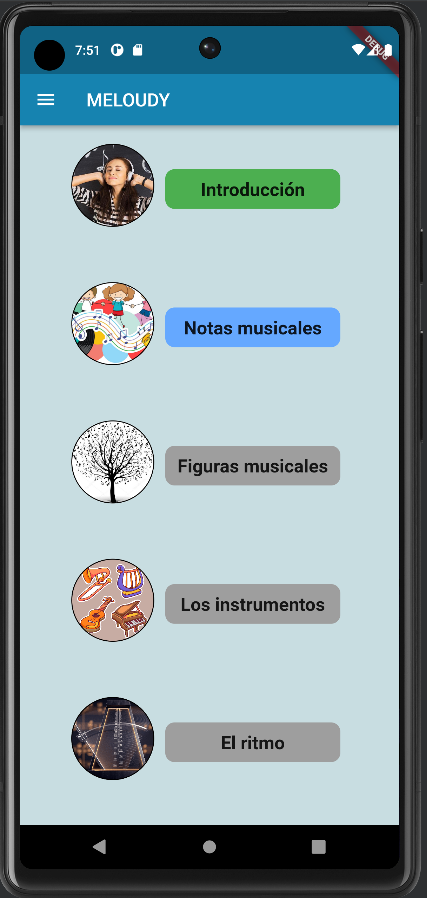
\includegraphics[width=0.40\textwidth]{imagenes/c7/pantprin.png} }}%
  \qquad
  \subfloat[\centering Estructura en componentes de la pantalla de lecciones.]{{ 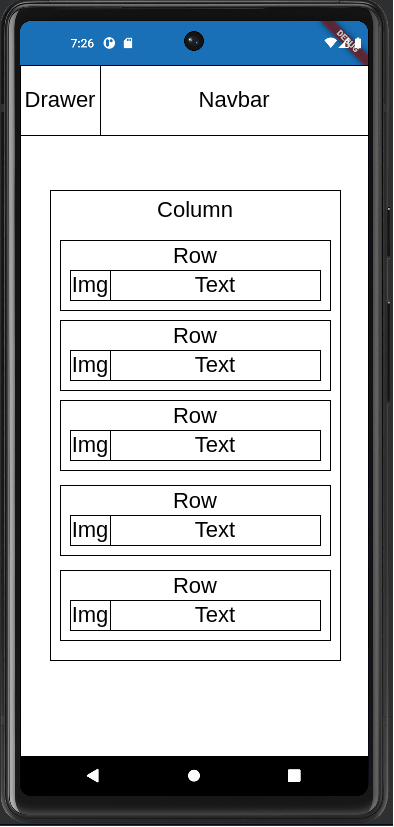
\includegraphics[width=0.406\textwidth]{imagenes/c7/leccionescompo.png} }}%
  \caption{Pantalla de la lista de lecciones con el título y la imagen de cada lección.}%
  \label{fig:login}%
\end{figure}


\paragraph*{Vista}
Para que el usuario pueda ver la lista de lecciones, se ha desarrollado un widget principal para la pantalla. Este widget contiene el widget \textit{ListaLecciones}, que contiene un componente para la distribución de widgets en una columna. Cada uno de estos widgets se llama \textit{LeccionItem} y contendrá la información principal de una lección, como el título y la imagen de perfil. En la figura anterior se puede ver la pantalla de lista de lecciones.

\paragraph*{Lógica}
Para la lógica de esta pantalla se ha utilizado el patrón de diseño \textit{Provider} para la gestión de estados. Un provider es un objeto que se encarga de gestionar el estado de la aplicación y proporcionarselo a los widgets que lo necesiten.
En este caso, se ha utilizado para gestionar el estado de la lista de lecciones y se le ha llamado \textit{Lecciones}.
Este Provider se encarga de obtener la lista de lecciones de la API (llamada HTTP con el verbo GET a la ruta (\textit{GET /api/lesson/get-lessons/\{id\}})) y almacenar cada uno de sus elementos en variables de la clase \textit{Lección}. Además, se ha creado un método público que devuelve la lista de lecciones. Este método se utiliza en el widget \textit{ListaLecciones} para obtener la lista de lecciones, añadir cada lección en forma de widget de forma iterativa
 y mostrarla en pantalla. 

\subsection{Lección} 
\textit{Desarrollado en el Sprint 5}
\label{sec:leccion}

La aplicación cuenta con una vista para cada lección. Esta vista se puede acceder pulsando en el título o en la imagen de una lección en la lista de lecciones. En esta vista se puede ver el contenido de la lección, como el título, el texto, las imágenes, los vídeos, etc.
Además, al final de la lección se puede hacer un test para comprobar los conocimientos adquiridos y revisar los tests realizados anteriormente por el usuario.

\paragraph*{Vista}
La vista de una lección proporciona al usuario información más detallada de esta. En primer lugar se muestra la imagen de la lección y el título en un componente para distribuir widgets en una fila. (Un widget \textit{Row} compuesto de un \textit{Text} y un \textit{Image} ).
A continuación, se muestra el contenido de la lección en forma de texto, imágenes, vídeos, etc. Esto se ha conseguido construyendo widgets de forma dinámica dependiendo del tipo de contenido almacenado y añadiéndolos a un widget distribuidor en columna (\textit{Column}).
Finalmente, se muestra un botón en pantalla para poder hacer un test y otro para ver el historial de tests realizados, ambos mediante un widget \textit{ElevatedButton}.
En la siguiente imagen se puede ver la pantalla de una lección:


\begin{figure}[H]%
  \centering
  \subfloat[\centering Parte 1.]{{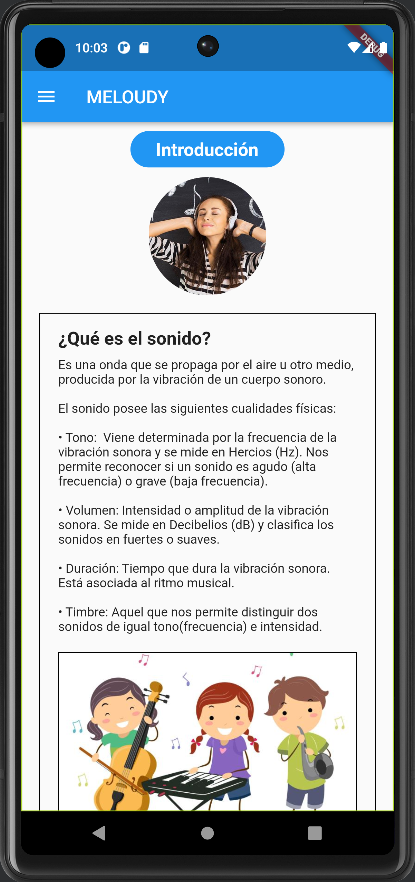
\includegraphics[width=0.44\textwidth]{imagenes/c7/leccion.png} }}%
  \qquad
  \subfloat[\centering Parte 2.]{{ 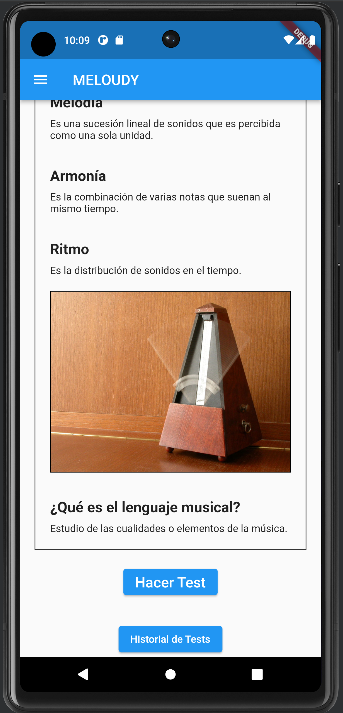
\includegraphics[width=0.44\textwidth]{imagenes/c7/leccion2.png} }}%
  \caption{Pantalla de una lección en concreto con los contenidos (títulos, texto, multimedia...) del temario y los dos botones relacionados con los tests.}%
  \label{fig:example}%
\end{figure}

\paragraph*{Lógica}
Para la lógica de esta pantalla se ha utilizado el provider \textit{Lecciones} mencionado anteriormente. En este caso, el provider se encarga de obtener la lección que se quiere mostrar en pantalla de la lista de lecciones y devolverla al widget que la mostrará en pantalla.
Además, se ha implementado una funcionalidad para poder construir el constenido de la lección de forma dinámica. Para esto se ha realizado un bucle que recorre el contenido de la lección y dependiendo del tipo de contenido, se construye un widget diferente. Por ejemplo, si el contenido es un texto, se construye un widget \textit{Text} y se añade a la lista de widgets que se devolverán al final del método. Si el contenido es una imagen, se construye un widget \textit{Image} y se añade a la lista de widgets que se devolverán al final del método. De esta forma 
se consigue que el contenido de la lección se muestre en pantalla en función del tipo y facilitaremos la adición de contenido a cada lección por parte del profesor en un futuro.

\subsection{Test}
\label{sec:test}
\textit{Desarrollado en el Sprint 6}

La lección contiene un test que se puede realizar al final de la lección. Este test consta de una serie de preguntas que el usuario deberá responder.

El usuario podrá responder a las preguntas de la siguiente forma: seleccionando una opción de la lista de opciones, seleccionando varias, escribiendo una respuesta en un campo de texto... El usuario podrá 
responder la opción que desee y pasar a la siguiente pregunta. A continuación se muestran las diferentes preguntas que se pueden realizar en el test.


\paragraph*{Vista}
La vista de un test consiste en una serie de preguntas que el usuario deberá responder. Al seleccionar el botón de \textit{Hacer Test} ubicado en la pantalla de la lección, se muestra la pantalla de un test.
En esta pantalla se presenta una pregunta a la vez, y el usuario deberá responderla. Para pasar a la siguiente pregunta, pulsará la flecha ubicada a la derecha de la imagen y para retroceder a la pregunta anterior, pulsará la flecha izquierda.
Esto se ha realizado mediante un widget que distribuye otros widget de forma horizontal en una fila (\textit{Row}). Este widget se encarga de mostrar la imagen de la pregunta actual y las flechas para pasar a la siguiente o anterior pregunta.

Debajo de lo anterior, se mostrará la pregunta actual y las opciones de respuesta. Esto se ha realizado mediante un widget que distribuye otros widget de forma vertical en una columna (\textit{Column}). 
Las opciones de respuesta dependerán del tipo de pregunta que se esté mostrando. Por ejemplo, si la pregunta es de selección única o múltiple, se muestra una lista de opciones de respuesta, mientras que si la pregunta es de entrada de texto, se muestra un campo de texto para que el usuario escriba su respuesta.

En la última pregunta, aparece un botón para enviar las respuestas y ver el resultado del test. Dicho botón evita que el usuario no pueda enviar las respuestas antes de responder o pasar por todas las preguntas.

\paragraph*{Lógica}
Para la lógica de esta pantalla se ha utilizado el patrón de diseño \textit{Provider} para la gestión del estado del test en curso.
Este Provider se encarga de obtener todas las preguntas del test de la API y almacenarlas en una lista privada. Para recorrer las preguntas, se ha utilizado un índice que se incrementa o decrementa en función de si el usuario quiere pasar a la siguiente o a la anterior pregunta. Este índice se almacena también en una variable privada e irá aumentando o disminuyendo en función de si el usuario quiere pasar a la siguiente pregunta o volver a la anterior.
Cada vez que el usuario responde una pregunta, se almacenan las respuestas en una variable privada para conservarlas durante toda la navegación del test (si vuelve para atrás, por ejemplo) y se produce una retroalimentación al usuario cambiando el color de la opción a un azul más oscuro para que el usuario sepa qué opción ha respondido.

Cuando el usuario pulsa el botón de enviar respuestas, estas se envían al servidor para crear el test y añadirlo al progreso (se envía la petición HTTP a la ruta de la API \textit{POST /api/progress/create-test-and-progress/}:) y aparece la pantalla
para ver el resultado del test.


\newpage 

\subsubsection{Pregunta de selección única.}\mbox{}\\

\label{sec:pregunic1}
\textit{Desarrollado en el Sprint 6}

A continuación se muestra la pantalla de una pregunta de selección única, en la que el usuario deberá seleccionar una opción de la lista de opciones:

\begin{figure}[H]%
  \centering
  \subfloat[\centering Selección única sin una respuesta seleccionada.]{{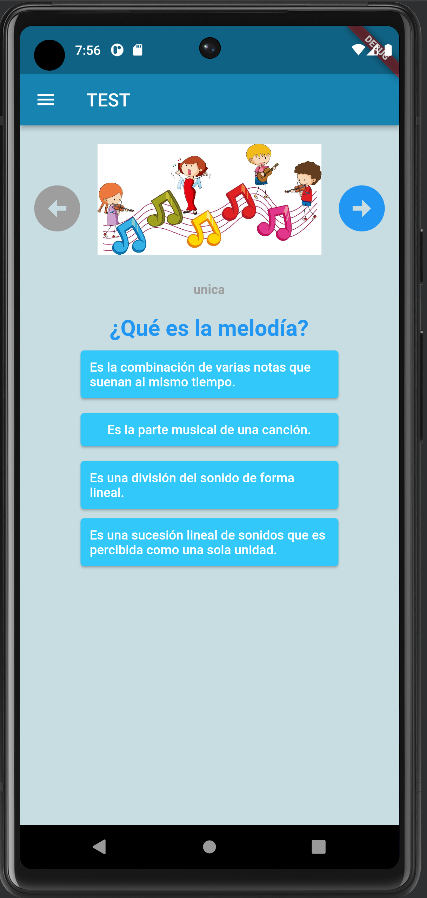
\includegraphics[width=0.45\textwidth]{imagenes/c7/selecunica.png} }}%
  \qquad
  \subfloat[\centering Selección única con una respuesta seleccionada.]{{ 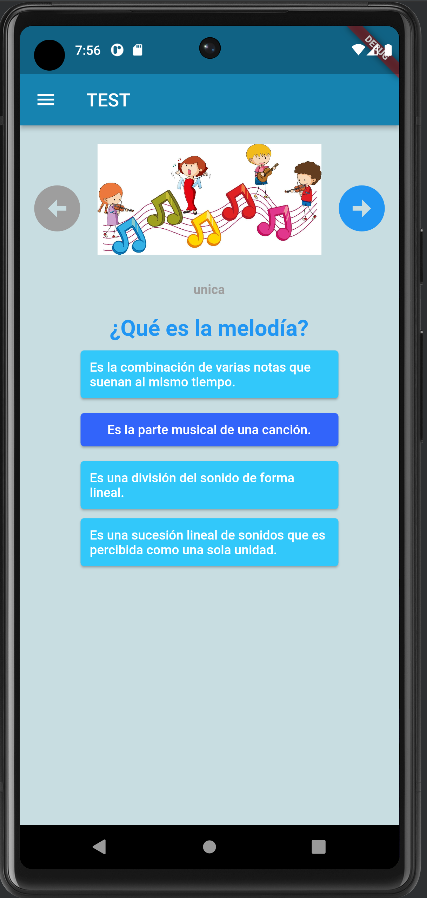
\includegraphics[width=0.45\textwidth]{imagenes/c7/selecunica2.png} }}%
  \caption{Pantalla de una pregunta de selección única en la que las opciones se muestran en forma de lista.}%
  \label{fig:example}%
\end{figure}

\newpage

\subsubsection{Pregunta de selección múltiple}\mbox{}\\

\label{sec:pregunic1}
\textit{Desarrollado en el Sprint 6}

A continuación se muestra la pantalla de una pregunta de selección múltiple, en la que el usuario deberá seleccionar una o varias opciones de la lista de opciones:

\begin{figure}[H]%
  \centering
  \subfloat[\centering Selección múltiple sin una respuesta seleccionada.]{{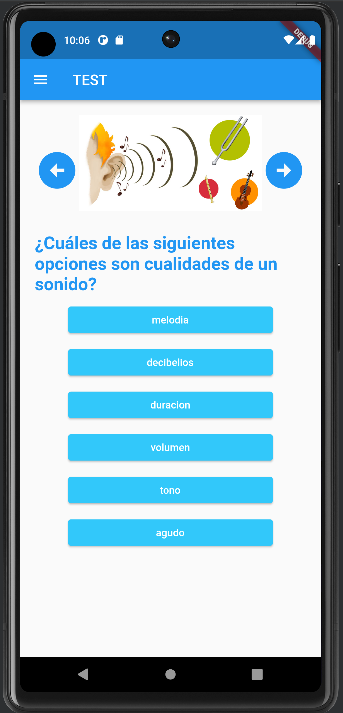
\includegraphics[width=0.45\textwidth]{imagenes/c7/selecmulti.png} }}%
  \qquad
  \subfloat[\centering Selección múltiple con varias respuestas seleccionadas.]{{ 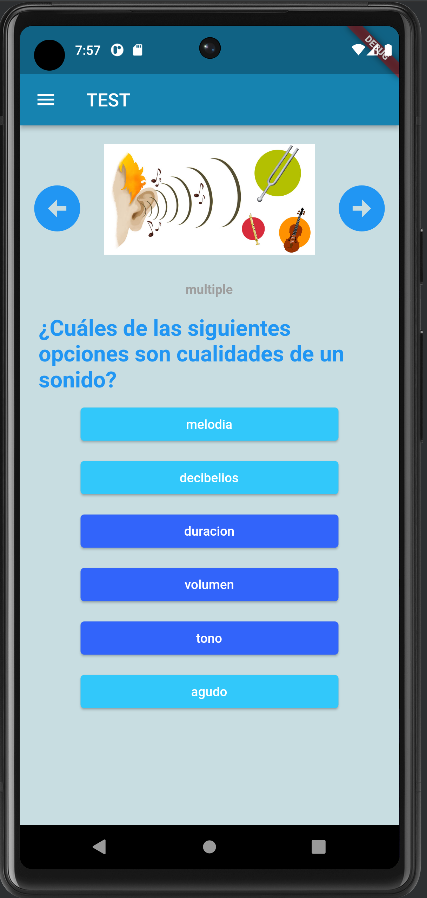
\includegraphics[width=0.45\textwidth]{imagenes/c7/selecmulti2.png} }}%
  \caption{Pantalla de una pregunta de selección múltiple en la que las opciones se muestran en forma de lista.}%
  \label{fig:example}%
\end{figure}



\newpage

\subsubsection{Pregunta de entrada de texto}

\label{sec:pregunic1}
\textit{Desarrollado en el Sprint 6}

A continuación se muestra la pantalla de una pregunta de entrada de texto, en la que el usuario deberá escribir la respuesta en un campo de texto:

\begin{figure}[H]%
  \centering
  \subfloat[\centering Entrada de texto sin respuesta introducida.]{{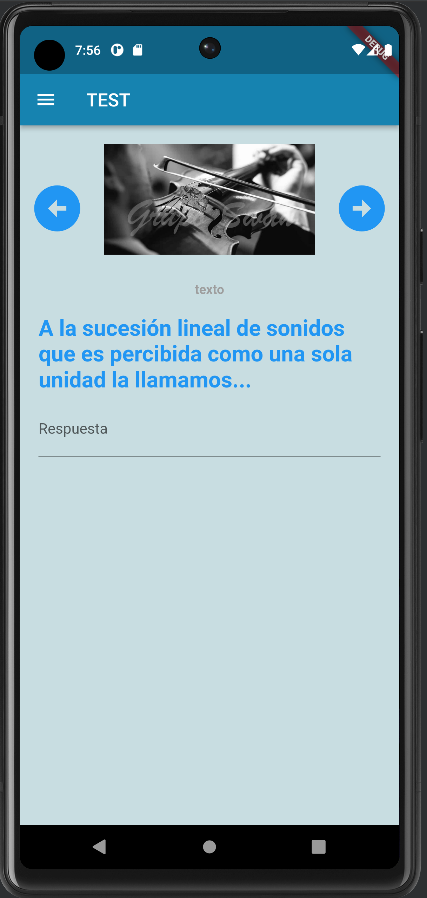
\includegraphics[width=0.45\textwidth]{imagenes/c7/entradatexto.png} }}%
  \qquad
  \subfloat[\centering Entrada de texto con respuesta introducida.]{{ 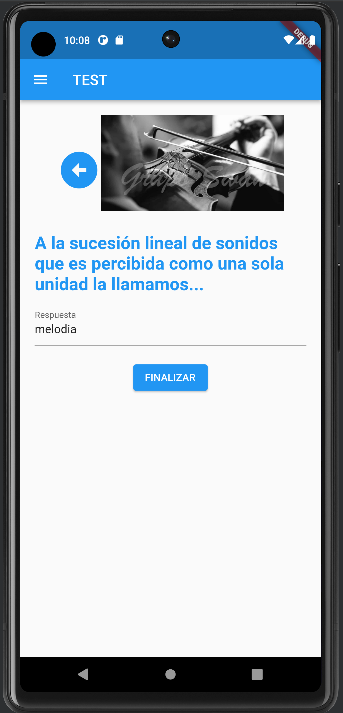
\includegraphics[width=0.45\textwidth]{imagenes/c7/entradatexto2.png} }}%
  \caption{Pantalla de una pregunta de entrada de texto. }%
  \label{fig:example}%
\end{figure}

\newpage
\subsubsection{Pregunta de micrófono}

\label{sec:pregunic1}
\textit{Desarrollado en el Sprint 7}

A continuación se muestra la pantalla de una pregunta de micrófono, en la que el usuario deberá grabar la respuesta mediante el micrófono del dispositivo. Esta respuesta
debe ser fiel a la partitura que se muestra en la imagen de la pregunta. 

\begin{figure}[H]%
  \centering
  \subfloat[\centering Pregunta de micrófono sin respuesta introducida.]{{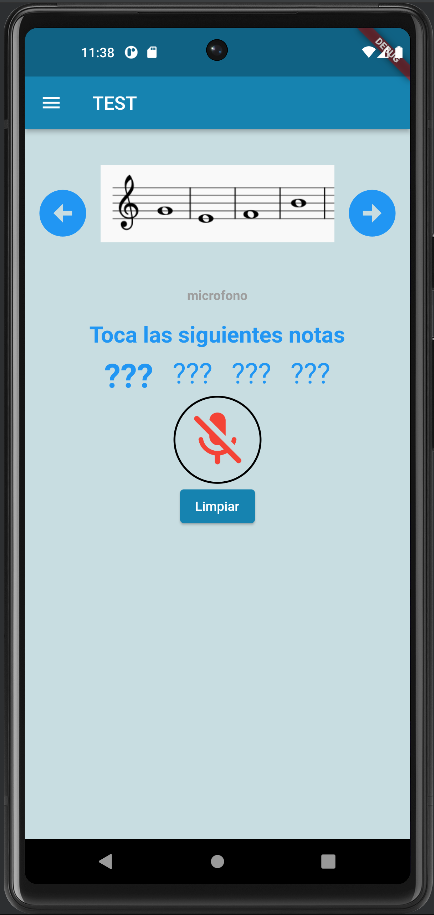
\includegraphics[width=0.45\textwidth]{imagenes/c7/entradamicrofono.png} }}%
  \qquad
  \subfloat[\centering Pregunta de micrófono introduciendo respuesta.]{{ 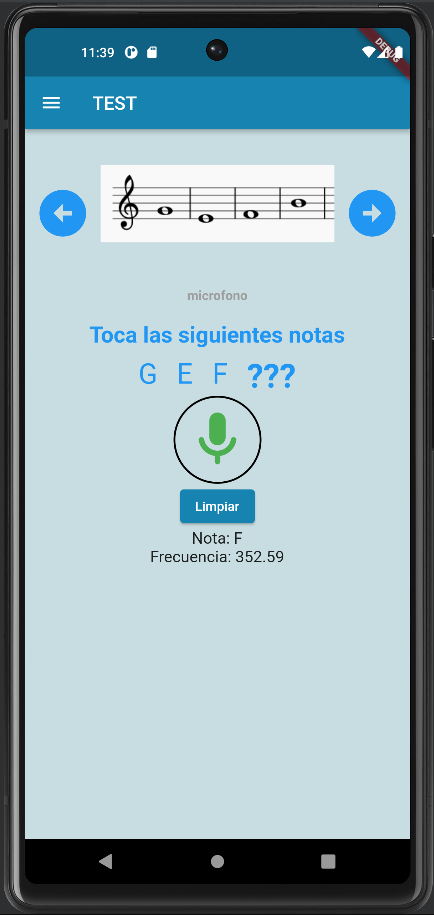
\includegraphics[width=0.45\textwidth]{imagenes/c7/entradamicrofono2.png} }}%
  \caption{Pantallas de una pregunta de micrófono. }%
  \label{fig:example}%
\end{figure}

\begin{figure}[H]
  \centering
  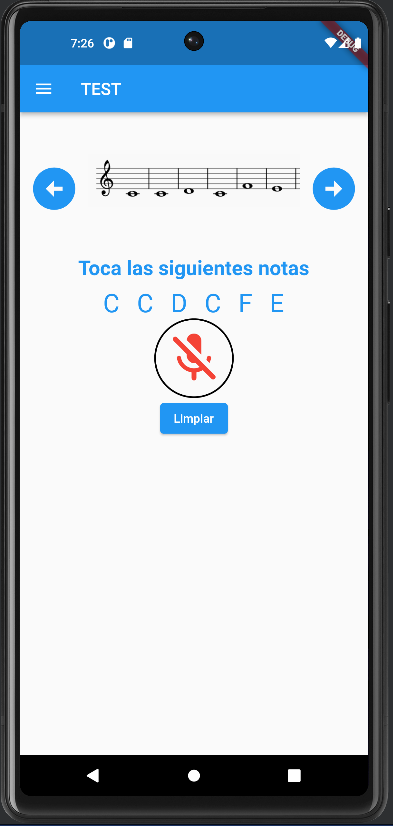
\includegraphics[width=0.4\textwidth]{imagenes/c7/entradamicrofono3.png}
  \caption{Pregunta de micrófono con respuesta introducida.}
  \label{fig:login}
\end{figure}

\paragraph*{Lógica}
Para realizar la lógica de esta pantalla se ha utilizado la biblioteca \textit{flutter\_fft}, que permite realizar la transformada de Fourier de una señal de audio.
Esta biblioteca permite obtener la frecuencia de la señal de audio, que se utiliza para determinar el tono del sonido, y obtener la nota musical que se está reproduciendo a partir de dicho valor de frecuencia.
Para ello, la biblioteca utiliza un \textit{StreamBuilder} que se encarga de obtener la frecuencia de la señal de audio. 
Se han realizado algunas modificaciones al código de la biblioteca para que la detección de notas sea más precisa y se pueda obtener la nota musical real que se está reproduciendo (había cierto desajuste que detectaba medio semitono más de lo que se estaba tocando).

Cabe mencionar que \textit{flutter\_fft} se le pueden ajustar varios parámetros para que la detección de notas sea más o menos precisa, como el número de muestras que se toman por segundo, el tiempo de espera entre muestras, etc.

Cuando el usuario pulsa el botón del micrófono, se inicia el \textit{StreamBuilder}, se cambia el estado del widget para establecer que se está grabando (variable isRecording) y se muestra una retroalimentación
al usuario cambiando el color del botón para notificar al usuario.

Además, las notas musicales se muestran en pantalla conforme el algoritmo las identifica. De esta manera, el usuario puede comprobar la exactitud de su interpretación en tiempo real.
Cuando se completan todas las notas de la partitura, se detiene el \textit{StreamBuilder} automáticamente.
Además, en el momento en el que el usuario pulsa el botón del micrófono cuando esté esta grabando, también se detiene el \textit{StreamBuilder}.

Si el usuario no está conforme con la respuesta, puede pulsar el botón de "Reiniciar" para resetear el ejercicio y puede volver a grabar pulsando el botón de micrófono. Por otro lado, si está conforme, puede pulsar el botón de siguiente para pasar a la siguiente pregunta.

\subsubsection{Resultado del test}
\label{sec:pregunta}
\textit{Desarrollado en el Sprint 6}

A continuación se muestra la pantalla de resultado del test, en la que se muestra el número y el porcentaje de aciertos respecto a las preguntas. Además, se muestra una barra de progreso que muestra el porcentaje de aciertos respecto al número de preguntas preguntas.

\begin{figure}[H]%
  \centering
  \subfloat[\centering Resultado aprobado (50\% o más).]{{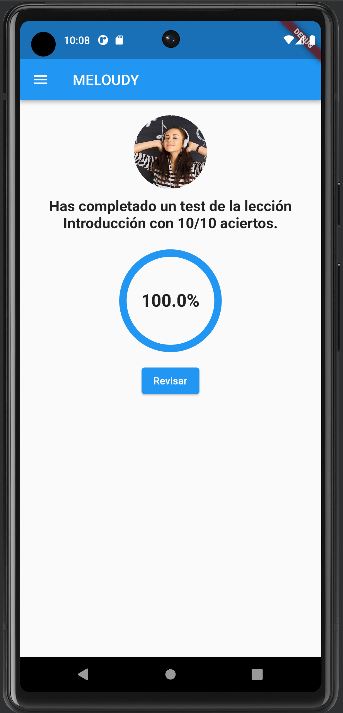
\includegraphics[width=0.45\textwidth]{imagenes/c7/porcentaje.png} }}%
  \qquad
  \subfloat[\centering Resultado suspenso (menos del 50\%).]{{ 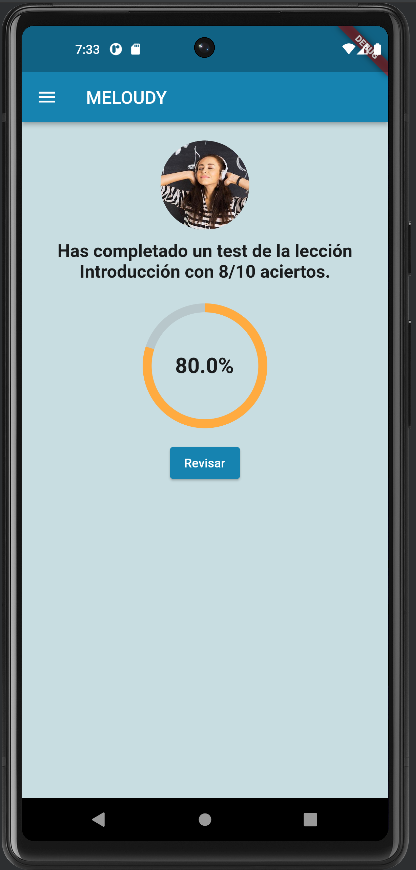
\includegraphics[width=0.45\textwidth]{imagenes/c7/porcentaje2.png} }}%
  \caption{Pantalla que muestra el resultado del test con el número de aciertos y el porcentaje de aciertos respecto a las preguntas con un Progress Bar.}%
  \label{fig:example}%
\end{figure}

\paragraph*{Vista}
\label{sec:vista}

Para realizar la vista de la pantalla se ha utilizado de nuevo el widget \textit{Column} para poder mostrar los elementos de la pantalla de forma vertical. 
Dentro de dicho widget tendremos:
\begin{itemize}
  \item la imagen de la lección (widget \textit{Image}).
  \item un campo de texto para mostrar el número de aciertos (widget \textit{Text}).
  \item una barra de progreso para mostrar el porcentaje de aciertos (widget \textit{CircularPercentIndicator}). Para este test se ha utilizado la biblioteca de flutter \textit{percent\_indicator}.
  \item un botón para poder revisar el test (widget \textit{ElevatedButton}).
\end{itemize}

\paragraph*{Lógica}
\label{sec:logica}
La lógica para mostrar el resultado del test es bastante sencilla.
Tras el envío del test al servidor, se comparan las respuestas del usuario con las respuestas correctas almacenadas en cada una de las preguntas (estas últimas se obtienen mediante el Provider de las preguntas). 
Una vez obtenidos estos datos, se calcula el porcentaje de aciertos y se envía a la vista.



\subsection{Revisar pregunta}
\label{sec:pregunta}
El usuario podrá revisar las preguntas que haya contestado en un test. Como se puede ver en la pantalla anterior del resultado del test, existe un botón para poder revisarlo. El usuario podrá ver las preguntas que haya contestado y las respuestas que haya seleccionado con la validación de estas.

\paragraph*{Vista}
\label{sec:vista}
La vista de la pantalla de revisión de preguntas es muy similar a la vista de la pantalla de la pregunta. La diferencia es que se muestran las respuestas que ha seleccionado el usuario si son correctas o no.
Por tanto, solo se han cambiado los colores de los botones y de los textos para mostrar si la respuesta es correcta o no.

\paragraph*{Lógica}
\label{sec:logica}
La lógica para mostrar la revisión de las preguntas se ha realizado comparando las respuestas del usuario con las respuestas correctas almacenadas en cada una de las preguntas (estas últimas se obtienen mediante el Provider de las preguntas).

Para mostrar si la respuesta es correcta o no, se ha cambiado el color del botón o del campo de texto. Si la respuesta es correcta, se muestra en verde y, si es incorrecta, se muestra en rojo. 

Para la validación, se ha llamado a la función \textit{validarRespuesta} que se ha creado en la clase provider \textit{Preguntas}. Esta función comprueba si la(s) respuesta(s) del usuario de la pregunta actual coincide con la(s) respuesta(s) correcta(s). En caso de hacerlo, se devuelve un valor booleano \textit{true}, y si no coincide, se devuelve un valor booleano \textit{false}.

Para mostrar el color de los botones o de los campos de texto, se ha utilizado la función \textit{ternario} de Dart. Esta función recibe tres parámetros: una condición, un valor si la condición es \textit{true} y un valor si la condición es \textit{false}. En nuestro caso, la condición es la función \textit{validarRespuesta} que hemos creado antes. Si la condición es \textit{true}, se devuelve el color verde, y si es \textit{false}, se devuelve el color rojo.

\newpage

\subsubsection{Revisión de pregunta de selección única}
\label{sec:pregunic1b}
\textit{Desarrollado en el Sprint 6}

\begin{figure}[H]%
  \centering
  \subfloat[\centering Revisión de selección única acertada.]{{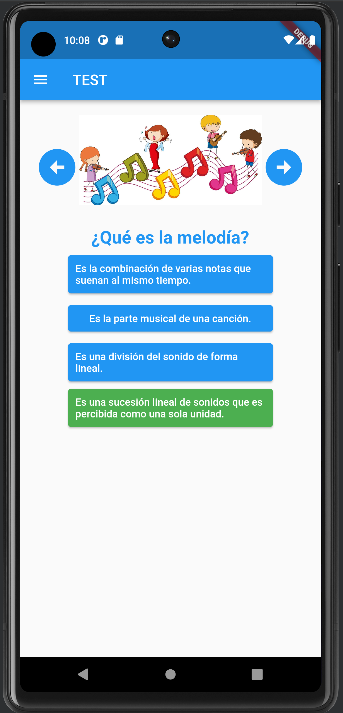
\includegraphics[width=0.45\textwidth]{imagenes/c7/selecunicab.png} }}%
  \qquad
  \subfloat[\centering Revisión de selección única fallida.]{{ 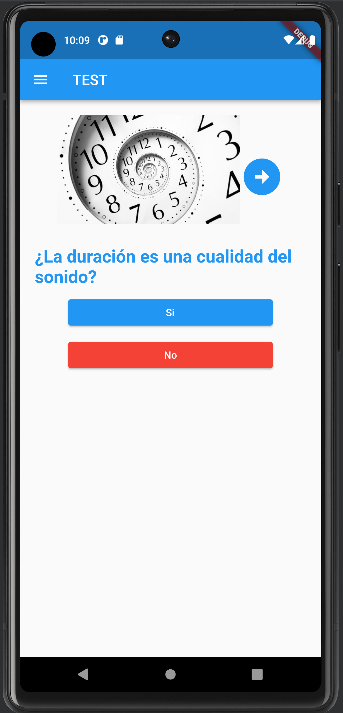
\includegraphics[width=0.45\textwidth]{imagenes/c7/selecunicab2.png} }}%
  \caption{Pantalla de la pregunta de selección única en revisión.}%
  \label{fig:example}%
\end{figure}

\newpage

\subsubsection{Revisión de pregunta de selección múltiple}\mbox{}\\
\label{sec:pregunic1b}
\textit{Desarrollado en el Sprint 6}

\begin{figure}[H]%
  \centering
  \subfloat[\centering Selección múltiple acertada.]{{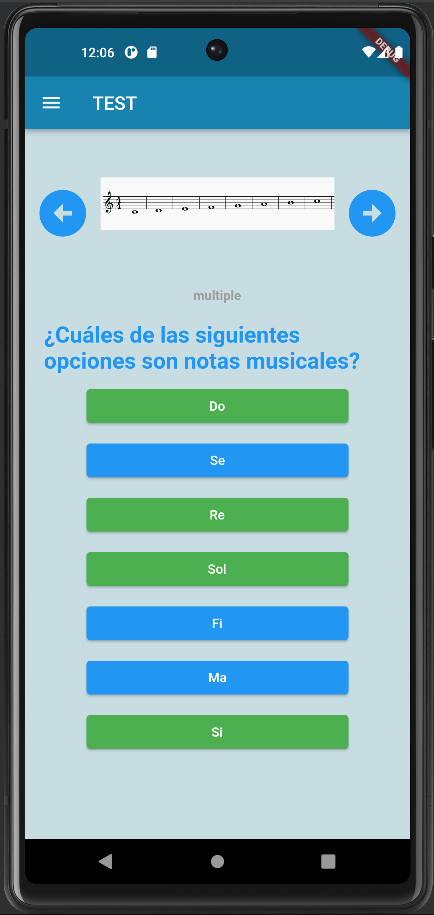
\includegraphics[width=0.45\textwidth]{imagenes/c7/selecmultib.png} }}%
  \qquad
  \subfloat[\centering Selección múltiple fallida.]{{ \includegraphics[width=0.45\textwidth]{imagenes/c7/selecmultib2.png} }}%
  \caption{Pantalla de la pregunta de selección múltiple en revisión.}%
  \label{fig:example}%
\end{figure}

\newpage

\subsubsection{Revisión de pregunta de entrada de texto}\mbox{}\\

\label{sec:pregunic1b}
\textit{Desarrollado en el Sprint 6}
\begin{figure}[H]%
  \centering
  \subfloat[\centering Revisión de entrada de texto acertada.]{{\includegraphics[width=0.45\textwidth]{imagenes/c7/entradatextob.png} }}%
  \qquad
  \subfloat[\centering Revisión de entrada de texto fallida.]{{ \includegraphics[width=0.45\textwidth]{imagenes/c7/entradatextb2.png} }}%
  \caption{Pantalla de la pregunta de entrada de texto en revisión.}%
  \label{fig:example}%
\end{figure}

\newpage

\subsubsection{Revisión de pregunta de entrada de micrófono}\mbox{}\\

\label{sec:pregunic1b}
\textit{Desarrollado en el Sprint 7}
\begin{figure}[H]%
  \centering
  \subfloat[\centering Revisión de entrada de micrófono acertada.]{{\includegraphics[width=0.45\textwidth]{imagenes/c7/entradamicrofonob2.png} }}%
  \qquad
  \subfloat[\centering Revisión de entrada de micrófono fallida.]{{ \includegraphics[width=0.45\textwidth]{imagenes/c7/entradamicrofonob.png} }}%
  \caption{Pantalla de la pregunta de entrada de micrófono en revisión.}%
  \label{fig:example}%
\end{figure}

\subsection{Historial de tests}
\textit{Desarrollado en el Sprint 6}
\label{sec:historial}

\paragraph*{Vista}
\label{sec:vista}
La vista de esta pantalla consiste en un distribuidor de columnas (Column) que contiene una lista de tests (ListView) verticalmente. 

\begin{figure}[H]
  \centering
  \includegraphics[width=0.4\textwidth]{imagenes/c7/historialtest.png}
  \caption{Pantalla de dashboard del profesor con las opciones de gestión disponibles para el profesor.}
  \label{fig:login}
\end{figure}


\newpage

\section{Funcionalidad del profesor}

\subsection{Dashboard}
\textit{Desarrollado en el Sprint 5}
\label{sec:dashboard}

Un dashboard es una interfaz de usuario que muestra información de forma resumida y que permite al usuario acceder a las diferentes funcionalidades de la aplicación. En este caso, el dashboard del profesor muestra las opciones de gestión de lecciones y preguntas.

\paragraph*{Vista}
Se ha implementado una pantalla de dashboard para la gestión de la aplicación. En esta pantalla, se muestran las opciones de gestión disponibles para la persona que utiliza la aplicación en función de su rol mediante una columna de ElevatedButton. En la siguiente imagen se puede ver la pantalla de dashboard:

\begin{figure}[H]
  \centering
  \includegraphics[width=0.45\textwidth]{imagenes/c7/dashboard.png}
  \caption{Pantalla de dashboard del profesor con las opciones de gestión disponibles para el profesor.}
  \label{fig:login}
\end{figure}

\newpage

\subsection{Lista de lecciones} 
\textit{Desarrollado en el Sprint 5}

\paragraph*{Vista}
La lista de lecciones del profesor es muy similar a la del usuario. Las diferencias, aparte de los estilos, son los botones de tipo ElevatedButton que se han añadido para la gestión de las lecciones y que permiten al profesor crear, modificar y eliminar lecciones. En la siguiente imagen se puede ver la pantalla de lista de lecciones del profesor:

\begin{figure}[H]
  \centering
  \includegraphics[width=0.45\textwidth]{imagenes/c7/listalecciones.png}
  \caption{Pantalla de lista de lecciones del profesor para la gestión de estas.} 
  \label{fig:login}
\end{figure}

\newpage

\subsection{Borrar lección} 
\textit{Desarrollado en el Sprint 8}
El profesor podrá borrar una lección de la lista de lecciones al pulsar el icono de la papelera mostrado en la vista del apartado anterior. Una vez pulsado, se mostrará un diálogo de confirmación para que el profesor confirme que desea borrar la lección.

\paragraph*{Vista}
La pantalla del borrado de lecciones utiliza el widget \textit{AlertDialog}, que posee
un título, un texto descriptivo y dos botones: uno para cancelar el borrado y otro para confirmarlo.
En la siguiente imagen se puede ver la pantalla de borrado de lecciones:


\begin{figure}[H]
  \centering
  \includegraphics[width=0.5\textwidth]{imagenes/c7/borrarleccion.png}
  \caption{Pantalla de lista de lecciones del profesor para la gestión de estas.} 
  \label{fig:login}
\end{figure}

\paragraph*{Lógica}
Una vez el botón de \textit{Confirmar} es pulsado, se muestra un diálogo de confirmación para que el profesor confirme que desea borrar la lección. Si el profesor confirma.
Este borrado se realiza llamando a la función borrarLeccion() del provider \textit{Lecciones}. En dicha función se borrará la lección de la lista del provider y se actualizará la base de datos enviando
una petición DELETE a la API con el id de la lección a borrar. La ruta de la petición es \textit{DELETE /api/lesson/delete-lesson}.La API devolverá un código de estado 200 si la operación se ha realizado correctamente y se actualizará la lista de lecciones del provider. En caso contrario, se mostrará un mensaje de error.


\subsection{Crear lección} 
\textit{Desarrollado en el Sprint 8}

Los profesores podrán crear lecciones para que los usuarios puedan estudiarlas. Para ello, se ha implementado una pantalla de creación de lecciones que permite al profesor añadir títulos, textos explicativos y contenido multimedia a la lección. Una vez creada, la lección se añadirá a la lista de lecciones del profesor.


\paragraph*{Vista}
La vista de esta pantalla consiste en un formulario de creación de lecciones. Este formulario consta de:
\begin{itemize}
  \item Un campo de texto para el título de la lección.
  \item Un botón para subir la imagen de la lección.
  \item Un número variable de campos de texto para los títulos.
  \item Un número variable de campos de texto para los textos explicativos.
  \item Un número variable de botones (\textit{ElevatedButton}) para las imágenes.
  \item Un número variable de campos de texto para los vídeos.
\end{itemize}

Todo esto está distribuido mediante el widget que organiza los elementos de forma vertical llamado \textit{Column}. 
En la parte inferior de la pantalla, se encuentran varios iconos organizados en una fila, que permiten incorporar nuevas widgets al contenido de la lección
ya que pulsando en uno de estos iconos, se añade un nuevo widget a la lista.

\newpage
En las siguientes imágenes se puede ver la pantalla de creación de lecciones:

\begin{figure}[H]%
  \centering
  \subfloat[\centering Creación de lección vacía \#1.]{{\includegraphics[width=0.45\textwidth]{imagenes/c7/crearleccion1.png} }}%
  \qquad
  \subfloat[\centering Creación de lección vacía \#2.]{{ \includegraphics[width=0.45\textwidth]{imagenes/c7/crearleccion2.png} }}%
  \caption{Pantalla de la creación de lecciones sin datos introducidos.}%
  \label{fig:example}%
\end{figure}


\begin{figure}[H]%
  \centering
  \subfloat[\centering Creación de lección rellena \#1.]{{\includegraphics[width=0.45\textwidth]{imagenes/c7/crearleccion1b.png} }}%
  \qquad
  \subfloat[\centering Creación de lección rellena \#2.]{{ \includegraphics[width=0.45\textwidth]{imagenes/c7/crearleccion2b.png} }}%
  \caption{Pantalla de la creación de lecciones con datos introducidos. }%
  \label{fig:example}%
\end{figure}

\paragraph*{Lógica}
La funcionalidad de crear lección ha necesitado desarrollar varias utilidades debido a su complejidad. 
La primera de ellas es la de añadir campos de texto a la pantalla de creación de lecciones. Para ello, se han creado varios widgets que contienen un campo de texto y un botón para eliminar dicho campo. Estos widgets se han llamado \textit{SubirTexto}, \textit{SubirTitulo} y \textit{SubirVideo} y se añaden de forma dinámica a un vector ubicado en la pantalla de creación de lecciones al pulsar el botón correspondiente.

Para subir una imagen se ha hecho uso de la biblioteca \textit{image\_picker}, que permite al usuario seleccionar una imagen de su galería y
devuelve la ruta de la imagen seleccionada. Una vez tenemos el archivo de la imagen, se manda una petición de tipo multipart con la imagen a la API para que la suba al servidor.
El almacenamiento de la imagen utiliza la funcionalidad proporcionada por el paquete de NodeJS llamado \textit{multer}. Este paquete permite la subida de archivos al servidor y la creación de carpetas para almacenar dichos archivos.
La ruta de la petición es \textit{POST /api/lesson/upload-image}. La API devolverá un código de estado 200 si la operación se ha realizado correctamente. En caso contrario, se mostrará un mensaje de error.

El profesor también podrá eliminar widgets de la pantalla de creación de lecciones. Para ello, se ha implementado un botón en cada widget que permite al profesor eliminar dicho widget. Al pulsar este botón, se llama al método borrar(). En este se elimina el widget de la lista y se actualiza la pantalla de creación de lecciones al ser un widget de tipo \textit{StatefulWidget}.

Una vez el usuario ha rellenado el formulario de creación de lecciones, se ha implementado un botón que permite al profesor guardar la lección. Al pulsar este botón, se envía una petición POST a la API con los datos de la lección. La ruta de la petición es \textit{POST /api/lesson/create-lesson}. La API devolverá un código de estado 200 si la operación se ha realizado correctamente y se actualizará la lista de lecciones del provider. En caso contrario, se mostrará un mensaje de error.


\subsection{Editar lección} 
\textit{Desarrollado en el Sprint 8}
Los profesores podrán editar la información y el contenido de las lecciones. Para ello, se ha implementado una pantalla de edición de lecciones que permite al profesor modificar el título, la imagen y todo el contenido.

\paragraph*{Vista}
La vista de esta pantalla es muy similar a la de la creación de lecciones. La diferencia es que los campos de texto continene la información de la lección que se está editando.

\begin{figure}[H]%
  \centering
  \subfloat[\centering Edición de lección \#1.]{{\includegraphics[width=0.4\textwidth]{imagenes/c7/editarleccion.png} }}%
  \qquad
  \subfloat[\centering Edición de lección \#2.]{{ \includegraphics[width=0.4\textwidth]{imagenes/c7/editarleccion2.png} }}%
  \caption{Pantalla de la edición de lecciones existentes por parte del profesor.}%
  \label{fig:example}%
\end{figure}


\paragraph*{Lógica}
En cuanto a la lógica, muchas de las funcionalidades de esta pantalla son iguales a las de la pantalla de creación de lecciones.

La única diferencia es que, al pulsar el botón de guardar, se envía una petición PUT a la API con los datos de la lección. La ruta de la petición es \textit{PUT /api/lesson/update-lesson}. La API devolverá un código de estado 200 si la operación se ha realizado correctamente y se actualizará la lista de lecciones del provider. En caso contrario, se mostrará un mensaje de error.

\newpage
\subsection{Lista de preguntas} 
\textit{Desarrollado en el Sprint 8}

\paragraph*{Vista}
La lista de preguntas contiene todas las preguntas existentes en el sistema. Se ha utilizado un distribuidor de columnas para mostrar las preguntas verticalmente. 
Cada pregunta tiene un distribuidor de elementos horizontal que contiene a la izquierda la imagen de la pregunta y a la derecha el texto de la cuestión, el tipo de pregunta y su identificador. 
Además de esto, cada pregunta tiene un icono de tipo Icon que permite al usuario modificar la pregunta.
\begin{figure}[H]
  \centering
  \includegraphics[width=0.4\textwidth]{imagenes/c7/listapreguntas.png}
  \caption{Pantalla de lista de preguntas del profesor para la gestión de estas.} 
  \label{fig:listapreguntas}
\end{figure}


\newpage
\subsection{Crear Pregunta} 
\textit{Desarrollado en el Sprint 9}

Los profesores podrán crear preguntas para que los usuarios puedan contestarlas en los tests. Para ello, se ha implementado una pantalla de creación de preguntas que permite al profesor elegir el tipo de pregunta y modificar toda la información relacionada con esta (imagen, opciones, respuestas correctas, etc). Una vez creada, la lección se añadirá a la lista de lecciones del profesor.



\paragraph*{Vista}
La vista de esta pantalla consiste en un formulario de creación de preguntas. Este formulario consta de:
\begin{itemize}
  \item Un desplegable para elegir el tipo de pregunta (entre \textit{única, múltiple, micrófono y texto}).
  \item Un botón para subir la imagen de la pregunta.
  \item Un desplegable para elegir la lección a la que pertenece la pregunta.
  \item Un campo de texto para el enunciado/cuestión de la pregunta.
  \item Si es una pregunta de tipo 'única' o 'múltiple', un número variable de campos de texto para las opciones de la pregunta.
  \item Si es una pregunta de tipo 'texto', un campo de texto para la respuesta correcta.
  \item Si es una pregunta de tipo 'micrófono', un número variable de desplegables para elegir las notas musicales correctas.
\end{itemize}




Todo esto está distribuido mediante el widget que organiza los elementos de forma vertical llamado \textit{Column}. Dentro de este, se encuentran los widgets del formulario, que serán desde widgets de desplegables (\textit{DropdownButton}) hasta widgets de campos de texto (\textit{TextField}), pasando por casillas de verificación (\textit{Checkbox}).
En las preguntas de tipo 'única', 'múltiple' y 'micrófono', en la parte inferior de la pantalla se encuentra un icono que permite al profesor añadir más opciones a la pregunta.

En las siguientes imágenes se puede ver la pantalla de creación de preguntas de todos los tipos con los campos de texto vacíos y rellenos.
\begin{figure}[H]
  \centering
  \includegraphics[width=0.32\textwidth]{imagenes/c7/crearpreguntaunica1.png}
  \caption{Pantalla de creación de pregunta de tipo 'única' vacía. La pregunta de tipo múltiple y de tipo micrófono son iguales.} 
  \label{fig:crearpreguntaunica}
\end{figure}


\begin{figure}[H]%
  \centering
  \subfloat[\centering Creación de pregunta 'única' rellena \#1.]{{\includegraphics[width=0.32\textwidth]{imagenes/c7/crearpreguntaunica2.png} }}%
  \qquad
  \subfloat[\centering Creación de pregunta 'única' rellena \#2.]{{ \includegraphics[width=0.32\textwidth]{imagenes/c7/crearpreguntaunica3.png} }}%
  \caption{Pantalla de creación de pregunta de tipo 'única' con datos introducidos.}%
  \label{fig:example}%
\end{figure}


\begin{figure}[H]%
  \centering
  \subfloat[\centering Creación de pregunta 'múltiple' rellena \#1.]{{\includegraphics[width=0.30\textwidth]{imagenes/c7/crearpreguntamultiple2.png} }}%
  \qquad
  \subfloat[\centering Creación de pregunta 'múltiple' rellena \#2.]{{ \includegraphics[width=0.30\textwidth]{imagenes/c7/crearpreguntamultiple3.png} }}%
  \caption{Pantalla de creación de pregunta de tipo 'múltiple' con datos introducidos.}%
  \label{fig:crearpreguntamultiple}%
\end{figure}



\begin{figure}[H]%
  \centering
  \subfloat[\centering Creación de pregunta 'micrófono' rellena \#1.]{{\includegraphics[width=0.30\textwidth]{imagenes/c7/crearpreguntamicrofono1.png} }}%
  \qquad
  \subfloat[\centering Creación de pregunta 'micrófono' rellena \#2.]{{ \includegraphics[width=0.30\textwidth]{imagenes/c7/crearpreguntamicrofono2.png} }}%
  \caption{Pantalla de creación de pregunta de tipo 'micrófono' con datos introducidos.}%
  \label{fig:crearpreguntamicrofono}%
\end{figure}

\begin{figure}[H]%
  \centering
  \subfloat[\centering Creación de pregunta 'texto' vacía.]{{\includegraphics[width=0.30\textwidth]{imagenes/c7/crearpreguntatexto1.png} }}%
  \qquad
  \subfloat[\centering Creación de pregunta 'texto' rellena.]{{ \includegraphics[width=0.30\textwidth]{imagenes/c7/crearpreguntatexto2.png} }}%
  \caption{Pantalla de creación de pregunta de tipo 'texto'.}%
  \label{fig:crearpreguntatexto}%
\end{figure}



\paragraph*{Lógica}
La funcionalidad de crear preguntas se ha implementado utilizando el Provider de preguntas anteriormente mencionado. De esta forma
se ha podido comunicar varias pantallas entre sí y compartir datos entre ellas. 

Para empezar, se ha creado un nuevo widget llamado \textit{SubirOpcion}, que actua de forma muy parecida a los widgets mencionados en la creación de lecciones (SubirImagen, SubirTitulo, SubirTexto...). Este widget se encargará de encapsular toda la vista y la lógica relacionada con una opción concreta.
Además he visto necesaria la creación de un nuevo Provider para las opciones de las preguntas. Este Provider contiene un vector de opciones y un vector de respuestas correctas.
El vector de opciones contiene los textos de las opciones de la pregunta y el vector de respuestas correctas contiene los índices de las opciones correctas.
Estos dos vectores se actualizan cada vez que el profesor añade o elimina una opción de la pregunta. De esta forma, la comunicación entre la pantalla y la clase "SubirOpcion" ha sido más sencilla tanto para borrar una opción como para desmarcar una opción cuando se marca otra distinta.
El widget de SubirOpcion se añade de forma dinámica a un vector de widgets ubicado en la pantalla de creación de preguntas al pulsar el botón correspondiente.


Para subir una imagen se ha hecho uso de nuevo de la biblioteca \textit{image\_picker}, que detallé en la funcionalidad de crear lecciones.
El profesor podrá eliminar widgets mediante el botón apropiado en cada uno de ellos. Dicho botón llama al método borrar() y éste elimina el widget de la listas y actualiza la pantalla de creación de preguntas.

El botón de guardar la lección envía los datos de las preguntas al servidor mediante una petición POST a la ruta /api/question/create-question. La API devolverá un código de estado 200 si la operación se ha realizado correctamente y se actualizará la lista de preguntas del provider. En caso contrario, se mostrará un mensaje de error.

\newpage

\subsection{Editar Pregunta} 
\textit{Desarrollado en el Sprint 9}
Los profesores podrán editar la información y el contenido de las preguntas. Para ello, se ha implementado una pantalla de edición de preguntas que permite al profesor modificar la cuestión, la imagen y todos los demás datos.

\paragraph*{Vista}
La vista de esta pantalla es muy similar a la de la creación de las preguntas. La diferencia es que los widgets disponen de la información de la pregunta que se está editando.

\begin{figure}[H]%
  \centering
  \subfloat[\centering Edición de pregunta única \#1.]{{\includegraphics[width=0.45\textwidth]{imagenes/c7/editarpreguntaunica1.png} }}%
  \qquad
  \subfloat[\centering Edición de pregunta única\#2.]{{ \includegraphics[width=0.45\textwidth]{imagenes/c7/editarpreguntaunica2.png} }}%
  \caption{Pantalla de edición de pregunta de tipo 'única'.}%
  \label{fig:edición_pregunta_unica}%
\end{figure}



\begin{figure}[H]%
  \centering
  \subfloat[\centering Edición de pregunta múltiple\#1.]{{\includegraphics[width=0.30\textwidth]{imagenes/c7/editarpreguntamultiple1.png} }}%
  \qquad
  \subfloat[\centering Edición de pregunta múltiple\#2.]{{ \includegraphics[width=0.30\textwidth]{imagenes/c7/editarpreguntamultiple2.png} }}%
  \caption{Pantalla de edición de pregunta de tipo 'múltiple'.}%
  \label{fig:edición_pregunta_multiple}%
\end{figure}


\begin{figure}[H]
  \centering
  \includegraphics[width=0.32\textwidth]{imagenes/c7/editarpreguntamicrofono.png}
  \caption{Pantalla de edición de pregunta de tipo 'micrófono'.} 
  \label{fig:edición_pregunta_microfono}
\end{figure}

\begin{figure}[H]
  \centering
  \includegraphics[width=0.32\textwidth]{imagenes/c7/editarpreguntatexto.png}
  \caption{Pantalla de edición de pregunta de tipo 'texto'.} 
  \label{fig:edición_pregunta_tecto}
\end{figure}


\paragraph*{Lógica}
En cuanto a la lógica, muchas de las funcionalidades de esta pantalla son iguales a las de la pantalla de creación de lecciones.
Entre las diferencias notamos que al entrar se deben inicializar los valores de cada uno de los campos con aquellos obtenidos de la base de datos y que, al pulsar el botón de guardar, se envía una petición PUT a la API con los datos de la pregunta. La ruta de la petición es \textit{PUT /api/question/update-question}. La API devolverá un código de estado 200 si la operación se ha realizado correctamente y se actualizará la lista de preguntas del provider. En caso contrario, se mostrará un mensaje de error.


   
   \chapter{Pruebas}

   
   \chapter{Conclusiones}

%
%%\chapter{Conclusiones y Trabajos Futuros}
%
%
%%\nocite{*}
%\bibliography{bibliografia/bibliografia}\addcontentsline{toc}{chapter}{Bibliografía}
%\bibliographystyle{miunsrturl}
%
%\appendix
%\input{apendices/manual_usuario/manual_usuario}
%%\input{apendices/paper/paper}
%\input{glosario/entradas_glosario}
% \addcontentsline{toc}{chapter}{Glosario}
% \printglossary
\chapter*{}
\thispagestyle{empty}

\end{document}
